\documentclass[ASNA,twocolumn]{USG}
\usepackage[utf8]{inputenc}
\usepackage{amsfonts}
\usepackage{amsmath}
\usepackage{amssymb}
\usepackage{longtable}
\usepackage{booktabs}
\usepackage{array}
\usepackage{tabularx}
\usepackage{ragged2e}
\usepackage{xltabular}
\usepackage{colortbl}
\usepackage{pdflscape}
\usepackage{bbm}
\usepackage{textgreek}
\usepackage{placeins}
\usepackage{float}

\definecolor{lightrowgray}{gray}{0.9}
\newcommand{\lightrowsep}{%
  \arrayrulecolor{lightrowgray}%
  \specialrule{0.30pt}{3.5pt}{3.5pt}%
  \arrayrulecolor{black}%
}

\graphicspath{{./images/}{./pictures/}}
\articletype{REVIEW ARTICLE}
\journal{Journal Manuscript}
\startpage{1}
\volume{}
\copyyear{2026}
\articledoi{}
\begin{document}
\title{A Comprehensive Review of EEG Based Emotion Recognition: Theories, Methods, Evaluation, and Emerging Trends}

\authormark{SARAR \textsc{et al.}}
\titlemark{A Comprehensive Review of EEG Based Emotion Recognition}
\author[1]{Shihab Sarar}[https://orcid.org/0009-0002-9989-8414]
\author[2]{Md Niaz Imtiaz}[https://orcid.org/0000-0002-3056-6756]
\author[3]{Naimul Khan}[https://orcid.org/0000-0002-8229-0747]
\address[1]{\orgdiv{Department of Computer Science and Engineering, }%
\orgname{Ahsanullah University of Science and Technology, }%
\orgaddress{\city{Dhaka}, \country{Bangladesh}}}
\address[2]{\orgdiv{Department of Computer Science and Engineering, }%
\orgname{Pabna University of Science and Technology, }%
\orgaddress{\city{Pabna}, \country{Bangladesh}}}
\address[3]{\orgdiv{Department of Electrical, Computer and Biomedical Engineering, }%
\orgname{Toronto Metropolitan University, }%
\orgaddress{\city{Toronto}, \state{Ontario}, \country{Canada}}}
\corres{Md Niaz Imtiaz (\email{niaz.cse@pust.ac.bd})}
\keywords{electroencephalography (EEG), emotion recognition, affective computing, deep learning, cross-subject learning, brain–computer interface (BCI), signal processing}


\abstract[ABSTRACT]{
    EEG based emotion recognition is a relatively new topic in the field of affective computing, which can enhance the ability of human–computer interaction and be used in the field of health care and adaptive technologies. EEG records the dynamics of emotions in the brain and offers information about emotions, which is difficult to obtain by using facial expressions and voice data. Even though there is considerable progress made in this field, comparing different studies is difficult due to differences in experiments, representation of signals, machine learning approaches, and evaluations. While some recent reviews focused on different aspects of EEG based emotion recognition, the relation between methods and generalization capabilities of models needs to be investigated more deeply. In this review, we cover the field from the neurophysiological bases of emotion recognition and emotion elicitation techniques to EEG recording, signal processing, feature extraction, and classification. We focus on the influence of all the mentioned factors on the reliability and generalization of models. In addition to traditional and deep learning methods, we cover data augmentation, transfer learning, and domain adaptation approaches to overcome the problem of limited amount of data and inter subject variability.
}


\historydates{}
\maketitle

\section{Introduction}

Emotion recognition is at the heart of models of human behavior, since emotional states directly and profoundly affect human cognition, decision making, and social interactions. Automatic emotion recognition facilitates the development of intelligent systems capable of adaptively responding to the affect states of users, and this is particularly critical in contemporary human computer interaction tasks \cite{moin2023multimodalhci}. Emotion recognition in psychology and neuroscience helps in the objective analysis of affective phenomena independently of subjective self assessments, and in the health sector, it paves the way for numerous tasks, such as the objective evaluation of mood disturbances, patient recovery, and supportive treatment of neurodevelopmental disorders such as autism and affect dysregulation \cite{miljevic2023depressionconnectivity}. Emotion recognition in engineering and brain computer interface studies helps in developing adaptive systems capable of automatically responding to the affective states of users \cite{gu2021bci}. Emotion recognition using EEG recordings is particularly useful in patient oriented tasks in the health sector, such as patient recovery and long term evaluation of patient moods, wherein overt behavioral manifestations of patients could be ambiguous and unavailing. EEG emotion recognition stands distinct, as it directly taps brain signals related to emotion recognition, and this makes the technology valuable in tasks where robustness and physiological validity of the detection tasks are critical .

Electroencephalography (EEG) is an approach used in non invasive neurophysiology in order to record the electrical activity of the brain at high speed, thus making possible the study of fast neuronal processes responsible for emotions. The use of physiological information, which adds value to behavioral information, especially when behavior is ambiguous or not enough, in emotion recognition through EEG is a field of research with applications in medicine \cite{li2018eegfeaturescross}.

EEG further provides important advantages compared to other emotion recognition methods, like facial expressions, speech, or body gestures. Behavioral cues are susceptible to intentional control, social camouflage, and context effects and are thus not very reliable in a sensitive context.  Conversely, EEG oscillations are symptomatic of inner neural activities that are hard to manipulate intentionally and supply objective estimations of affective states \cite{PeerJCS2065}. Although increasingly explored, at least for the future of emotion sensitive BCIs, multimodal approaches combining EEG with other physiological or behavioral signals are not required, and EEG alone can be a robust and informative modality owing to its direct sensitivity to emotional brain dynamics and the compatibility with BCI systems.

Despite its benefits, it still faces some difficulties when it comes to identifying emotions using EEG. The quality of EEG signals greatly depends on parameters such as electrode placement, skin conductivity, movement artifacts, and inconsistency across sessions. Inconsistencies resulting from variations in experimental methods, emotions, labels, and preprocessing make the task harder \cite{kukhilava2025evaluation}. This poses a challenge when trying to compare methodology based methods in order to evaluate their performance on various databases such as DEAP, SEED, and DREAMER \cite{katsigiannis2018dreamer}. Moreover, there are large differences between individuals leading to large changes in feature distributions of EEG signals.

The emergence of recent techniques in EEG based emotion recognition resulted in the appearance of various computational solutions that include traditional machine learning approaches using handcrafted features and deep learning solutions that automatically extract task related representations from EEG data. Deep learning solutions include convolutional neural networks (CNNs) for spatial patterns in EEG channels \cite{li2022efficientcnncl}, recurrent neural networks (RNNs) for modeling of brain activities temporal dynamics \cite{yang2018pcrnn}, and graph neural networks (GNNs) for modeling of inter brain regions' connections \cite{zhong2020rgnn}.

There has been an increased need to carry out a review of up to date research work in the area of emotion recognition using EEG. There are many reviews that were mainly concentrating on architectural originality or evaluation tasks on a single dataset, with less concern for cross subject and cross dataset generalization \cite{kukhilava2025evaluation}. Moreover, the lack of standard preprocessing methods and evaluation procedures makes it impossible to make reliable conclusions concerning the research \cite{li2022tutorial}. There is no common understanding of the best way to create models and evaluate them for EEG based emotion recognition \cite{geng2025dlreview}.

Past literature reviews have improved the understanding of emotion recognition via electroencephalogram (EEG) signals through their investigation into signal processing, features, learning, transfer learning, and experiments. Nevertheless, these factors tend to be studied independently without considering the interactions among them in relation to the neurophysiological properties, methodologies, and experiments used and what impact they have on the performance and generalizability of the EEG based emotion recognition process. To this end, this review integrates these aspects to explore the EEG based emotion recognition problem from a holistic perspective. The contributions of this review include the following:

\begin{enumerate}

  \item Connecting the neurophysiological bases to the methodology choices made: In this literature review, emotion theories, stimulus design, recording of EEG signals, and brain activations are linked to the later stages of recognition. The study of such connections reveals how the experimental setup and properties of recorded neural signals impact signal processing and modeling.

  \item Formulation of an integrated workflow centric framework for EEG emotion recognition: There are different frameworks that exist, each classified according to the various levels involved in emotion recognition such as pre processing, feature extraction/selection, modeling and evaluation. The dependencies of these stages are analyzed and described in order to show how decisions taken at one stage affect other stages.

  \item Synthesis of relationship between EEG representation and learning approaches: In this review, it is considered how temporal, spectral, spatial, and time frequency representations are used in classical machine learning approaches and neural networks such as convolutional, recurrent, graph based, attention based, and hybrid networks. The approaches depend on the type of information being used, their dependence on features of brain regions and frequency bands, and on their computational demand.

  \item Facilitating more meaningful comparisons through protocol aware evaluations: In this review, the impact of differences in datasets, emotion labeling, pre processing, and training testing protocols is considered in terms of the interpretation of reported results. This is done by looking at comparisons between subject dependent, subject independent, and transfer learning scenarios in relation to appropriate evaluation methods.

  \item Connecting key methodological problems with their solutions: The current review integrates the problem of feature redundancy, overfitting, lack of training data, and variability of subjects into one single list which is accompanied by the corresponding solution methods. The methods of feature selection, regularization, data augmentation, transfer learning, domain adaptation, domain generalization, and fine tuning are evaluated against their purpose of improving recognition accuracy.

  \item The requirements for applying experimental achievements in practice: Apart from classification accuracy, the analysis includes robustness, computational cost, channels needed, variability of recordings, and generalization on novel subjects. All these aspects define the research directions towards making EEG based emotion recognition more robust and applicable in practice.

\end{enumerate}

\begin{table*}[htb]
\centering
\normalsize
\renewcommand{\arraystretch}{1.2}
\setlength{\tabcolsep}{3pt}

\caption{Comparison of key research dimensions covered by recent reviews on EEG based emotion recognition.}
\label{tab:coverage_comparison_transposed}

\begin{tabular*}{\textwidth}{@{\extracolsep{\fill}}p{0.24\textwidth}*{8}{c}@{}}
\toprule

\textbf{Research Dimension} &
\shortstack{\textbf{Jafari et al.}\\
\textbf{2023}\\
\cite{jafari2023dlreview}} &
\shortstack{\textbf{Vempati and Sharma}\\
\textbf{2023}\\
\cite{vempati2023automatedeegreview}} &
\shortstack{\textbf{Erat et al.}\\
\textbf{2024}\\
\cite{erat2024mta}} &
\shortstack{\textbf{Wang et al.}\\
\textbf{2024}\\
\cite{wang2024csur_researchprogress}} &
\shortstack{\textbf{Ma et al.}\\
\textbf{2024}\\
\cite{PeerJCS2065}} &
\shortstack{\textbf{Geng et al.}\\
\textbf{2025}\\
\cite{geng2025dlreview}} &
\shortstack{\textbf{Chen et al.}\\
\textbf{2025}\\
\cite{chen2025asocreview}} &
\shortstack{\textbf{This}\\
\textbf{Work}} \\
\midrule

Emotion Theory
& -- & $\checkmark$ & $\checkmark$ & --
& -- & $\checkmark$ & -- & $\checkmark$ \\

Stimulus Design
& -- & -- & $\checkmark$ & --
& -- & -- & -- & $\checkmark$ \\

EEG Acquisition
& -- & -- & $\checkmark$ & --
& -- & $\checkmark$ & -- & $\checkmark$ \\

Multimodal Modeling
& -- & -- & -- & $\checkmark$
& -- & -- & -- & $\checkmark$ \\

Feature Fusion
& -- & -- & -- & $\checkmark$
& -- & -- & -- & $\checkmark$ \\

Data Augmentation
& -- & -- & -- & $\checkmark$
& -- & -- & -- & $\checkmark$ \\

Model Taxonomy
& $\checkmark$ & $\checkmark$ & $\checkmark$ & --
& $\checkmark$ & $\checkmark$ & $\checkmark$ & $\checkmark$ \\

Domain Adaptation
& -- & -- & -- & $\checkmark$
& $\checkmark$ & $\checkmark$ & -- & $\checkmark$ \\

Subject-Independent Evaluation
& -- & -- & -- & $\checkmark$
& $\checkmark$ & $\checkmark$ & -- & $\checkmark$ \\

Evaluation Reproducibility
& -- & -- & -- & --
& -- & -- & -- & $\checkmark$ \\

\bottomrule
\end{tabular*}

\vspace{2mm}
\begin{minipage}{\textwidth}
\footnotesize
\textit{Note:} $\checkmark$ indicates substantial coverage
of the specified research dimension, whereas  indicates
that the dimension is not treated as a distinct major focus.
The comparison reflects the thematic emphasis of the
reviewed articles rather than their scientific quality.
\end{minipage}

\end{table*}

As stated in Table \ref{tab:coverage_comparison_transposed}, the unique value of this review is based on an integrative examination of neurophysiological background, recognition processes, approaches to learning, evaluation techniques, and implementation issues. Such an approach allows for exploring connections between these aspects and for defining limitations which have not been fully addressed yet.

\section{Theoretical and Methodological Foundations}
The theoretical background defines EEG-based emotion recognition as a framework that links measurable neurophysiological activity to computational representations of affect. It models emotional state as a structured pattern distributed across time, frequency bands, and scalp locations, and it treats learning as the problem of extracting robust features or representations from noisy, non-stationary brain signals. The paper also shows two methods for using emotion labels including the following paradigms: the discrete classification paradigm in which EEG segments are classified into separate emotion states and the continuous modeling paradigm in which the prediction of valence and arousal is performed \cite{ma2024peerjreview}. These paradigms shape methodologies of design, evaluations and generalization of subjects and sessions \cite{li2022tcds_emotiontransfer_review}.

\subsection{Emotion Recognition}

Emotion detection is one of the basic goals of affective computing, which allows computer systems to detect and react to human emotions. The need for such technology has increased due to the increasing requirement for personalized and emotion aware human computer interaction (HCI) because of the possibility of improving the interaction of computer systems with users by detecting their affective state \cite{moin2023multimodalhci}. Conventional emotion recognition techniques rely on behavioral clues, such as facial expression, speech, gestures, and text. Nevertheless, the behavior can either be affected by the environment or can be hidden intentionally. However, physiological parameters offer more insights, which include the use of EEG to monitor brain activity, with emphasis on temporal resolution of the signal.

The EEG emotion detection is the act of detecting emotional states through the variations in the rhythmic and spatial dynamics of the brain due to emotional activities. This process is normally carried out by preprocessing, feature extraction through analysis of temporal, spectral, and time-frequency methods followed by machine learning. With the advancements in deep learning technology, it has been possible to extract complex spatiotemporal features automatically, thereby decreasing the reliance on manual feature engineering. However, individual differences, variation in data collection methods and protocol for emotion induction remain to be the challenge for achieving subject independence and cross dataset recognition of emotions, thus leading to the utilization of transfer learning and domain adaptation techniques \cite{hamzah2024heliyon}.

As such, EEG based emotion recognition is more than obtaining high classification accuracies. Signal representations, standard protocols, and generalization evaluations are the necessary components in creating affective computing systems.

\subsection{Neurophysiological Foundations of Emotional States}
Neurophysiological accounts of emotion in EEG emotion recognition interpret emotional episodes as changes in distributed brain activity that manifest as time varying and band limited oscillatory patterns across channels. EEG acquisition during affective stimulation, therefore, produces signals with spatial structure across electrode locations, temporal structure due to stimulus duration and sliding window segmentation, and frequency structure because analysis commonly separates δ, θ, α, β, and γ rhythms, each of which exhibits different responsiveness under affective conditions.

In this context, EEG based emotion recognition pipelines generally follow either a conventional sequence of denoising, feature extraction, and classifier training or an end to end learning approach. Both approaches depend on the availability of labeled data and the extent to which training and test samples satisfy the assumption of being independently and identically distributed (IID) \cite{li2022tcds_emotiontransfer_review}. When these assumptions fail especially under cross subject, cross session, or cross database settings emotion related neural patterns appear heterogeneous, motivating modeling strategies that explicitly target domain gaps and subject bias.
EEG emotion recognition surveys formalize feature construction as multi-domain representation learning. Temporal features describe transitory to long lasting changes in events, while spectral features include anything like Bandpass filtering, Fourier transformation, and other transformations like them. Spatial features describe interchannel relationships that correspond to the spatial organization of the cortical structure of the human brain and its variability. This multidomain stance links directly to contemporary architectures (CNN/RNN/GNN/Transformer variants) that operationalize spatial, temporal and spectral fusion and to transfer learning approaches that seek domain invariant representations under strong inter individual variability.

Benchmark datasets encode these neurophysiological assumptions by pairing affective stimuli like, videos or music with EEG recordings and either discrete labels or continuous ratings, thereby defining the target emotional state space and the evaluation protocol.

\subsubsection{Discrete Emotion Representation Models}
Discrete emotion theories categorize emotions in a class form that starts from the general positive, neutral, and negative emotions to discrete emotions like happiness, sadness, and anger. Classification in EEG emotion recognition is concerned with the separation of the emotional classes using the neural activities captured as EEG data over time, frequency, and electrodes.

Commonly used features are PSDs and DEs in different frequency bands and the spatial information of multiple electrodes. Conventional classifiers such as SVM and KNN use manually designed features, while deep learning methods automatically extract the EEG features. Spatial and spectral features can be learned using CNNs, while temporal features can be extracted using RNNs. Relations between different electrodes can be represented by GNNs, while attention and hybrid models combine these abilities \cite{zhong2020rgnn}.

\begin{figure}[h]
    \centering
    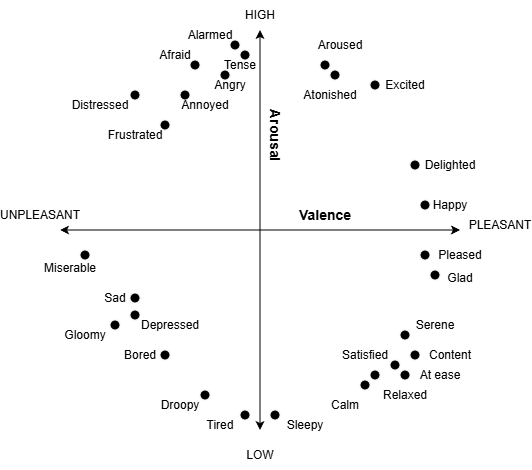
\includegraphics[width=\linewidth]{pictures/Valence.png}
    \caption{Conceptual representation of affective states in the two-dimensional valence-arousal space.}
    \label{fig:valence}
\end{figure}

Fig.~\ref{fig:valence} illustrates the valence-arousal space, in which emotional states are represented by their relative positions rather than isolated labels. Continuous ratings may also be divided into binary high/low classes or four valence--arousal quadrants, although these transformations discard some information about emotional intensity.

The recognition accuracy is also affected by the evaluation environment. While subject-dependent systems can take advantage of the patterns specific to an individual, subject-independent and cross-dataset classification needs to account for the variation in the EEG distributions. These changes can be overcome via transfer learning and domain adaptation, which involve the transfer of knowledge via instances, features, parameters, or relations. This implies that the usefulness of discrete emotion models is not limited to their classification performance alone.

\subsubsection{Continuous Dimensional Emotion Representation Models}

The continuous dimensional model represents emotions in terms of affective dimensions such as valence (pleasure) and arousal (activation), while dominance is sometimes included as an extra dimension. In contrast to the discrete emotion classification approach, this enables EEG-based emotion recognition systems to predict or classify the dimensions like, high or low valence or arousal.

Dimensional modeling of emotions is crucial for EEG emotion recognition as emotions are defined as a change of the neural activity over time. Hence, it becomes necessary to preprocess and segment the EEG signals before calculating the spectral or entropy features like PSD or DE or obtaining features from the raw data through machine learning methods.

\begin{figure}[h]
    \centering
    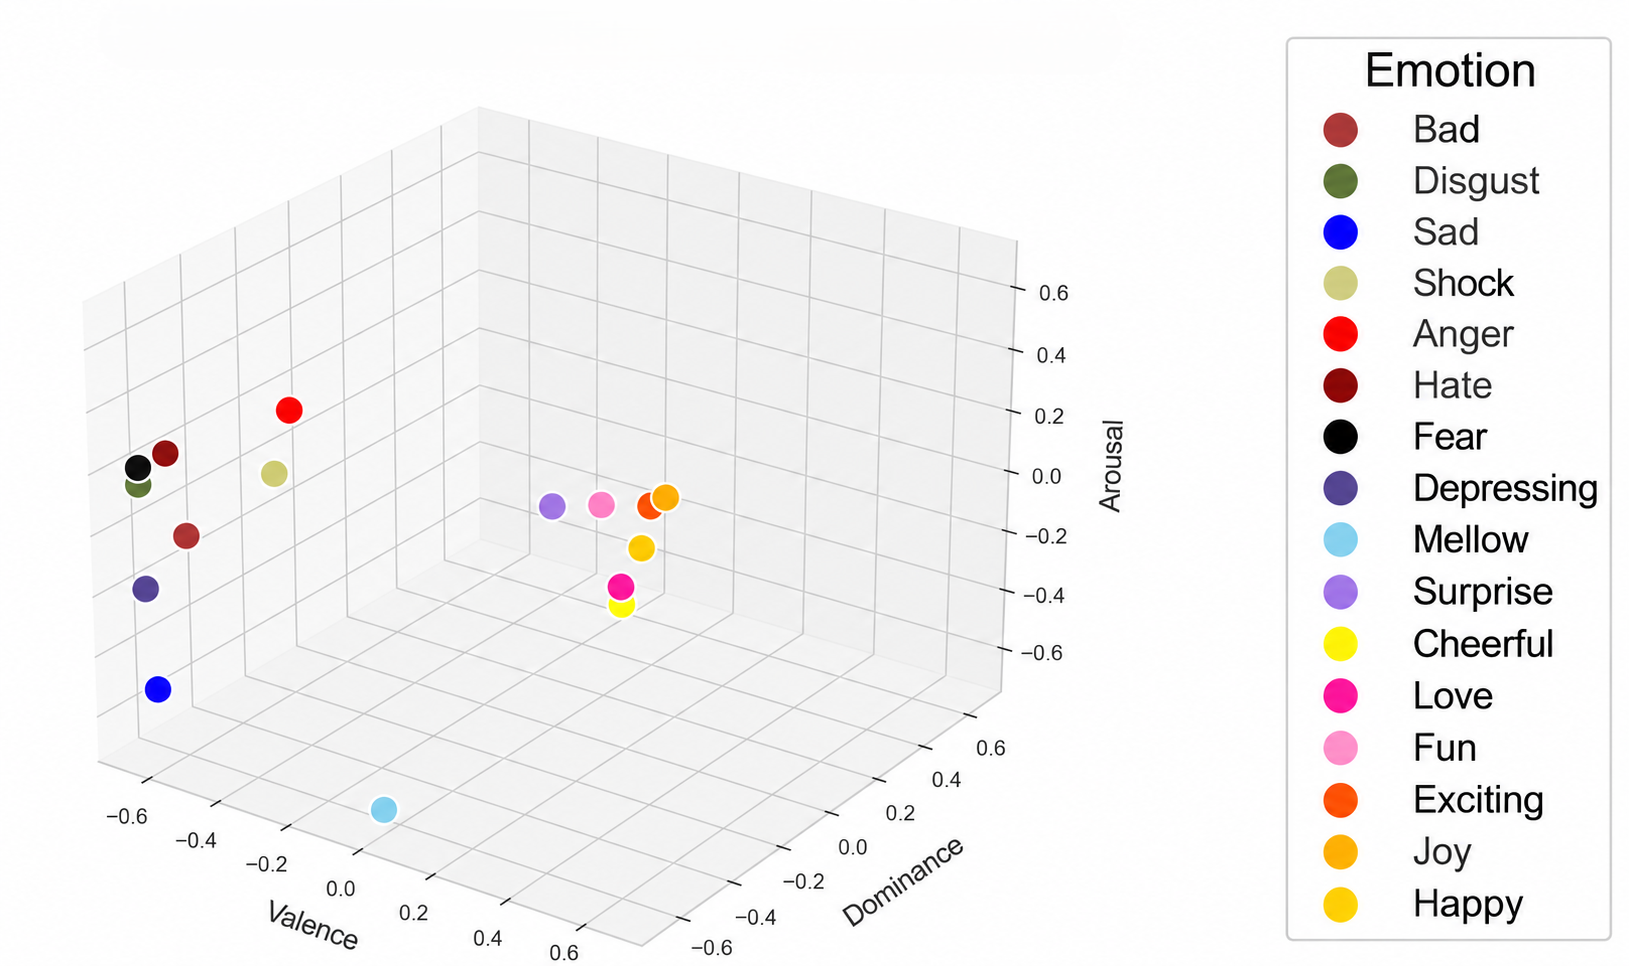
\includegraphics[width=\linewidth]{pictures/3D_emotion.png}
    \caption{Three dimensional representation of selected emotional states in the valence–arousal–dominance (VAD) space, illustrating their distribution across emotional pleasantness, activation, and perceived control.}
    \label{fig:vad_emotion_model}
\end{figure}


The three dimensional emotion model extends the traditional valence-arousal framework by introducing dominance as an additional dimension of emotional experience. Valence describes whether an emotion is pleasant or unpleasant, arousal indicates its level of activation, and dominance reflects the degree of control an individual perceives over the emotional experience. As illustrated in Fig.~\ref{fig:vad_emotion_model}, emotional states can be represented as distinct points within this three dimensional space, providing a more detailed description of their affective characteristics. By considering these dimensions together, the model offers a broader representation of emotional experiences, which can be useful for interpreting EEG responses and developing emotion recognition systems that account for variations in affective states.

A persistent limitation is the variability of EEG distributions and affective ratings across subjects, sessions, and datasets. Negative transfer is one possibility of distribution mismatches in transfer learning and domain adaptation that might hinder the process of generalization. Thus, successful dimensional modeling should involve reliable labels and proper preprocessing as well as evaluation processes of the model.

\subsection{Emotion Induction and Stimulus Design}

The induction method affects the way in which the affective state is induced, labeled, and compared to the EEG signal. Visual, auditory, and video stimuli are common due to controllable presentation times to allow trial separation and comparison among subjects \cite{alarcao2019eegsurvey,roy2019dleegreview}. Post-stimulus questionnaires are helpful in making a link between EEG recording and the experienced emotion by the subject \cite{jafari2023dlreview}.

Tasks and memories can trigger relevant emotions. However, the unpredictability and subjective nature of the stimuli make it hard to control the experiment. The choice of stimuli for an experiment should combine standardization, relevance, and ecological validity. When working on multimodal data, synchronizing readings from peripheral channels to EEG recording is important in order to identify the same response \cite{rayatdoost2020expressionguided}.

The differences in stimulus type and emotional induction procedure might create distributional shift between corpora, which would impair the ability of the model to generalize on different corpora \cite{rayatdoost2018crosscorpus}. The use of the new contrastive and self-supervised paradigms, on the other hand, further motivates designing experiments that allow for acquiring diverse and comparable EEG recordings for building robust affective representations \cite{shen2022contrastive}.

\subsection{Progress in Data Acquisition Technologies}

Improvements in acquisition of EEG data have allowed emotion recognition to move from laboratory settings towards wearable devices and mobile applications. While research-grade systems allow a greater number of electrodes and produce more reliable data, their high cost, need for preparation, and lack of portability can make their application difficult. Therefore, the choice of the device should take into account the quality of data, comfort of participants, and conditions of use, since the differences in acquisition methods may affect the performance of models \cite{gu2021bci}.

The number of electrodes and their placement define what regions of the scalp will be captured and how much spatial information will be available for classification. Fig. ~\ref{fig:eeg_electrode_placement} shows a multichannel configuration covering frontal, central, temporal, parietal, and occipital regions of the brain. The selection of relevant channels may also help in reducing the computation complexity of the models while preserving emotion-specific information \cite{zhang2024bfenet}.

\begin{figure}[t]
    \centering
    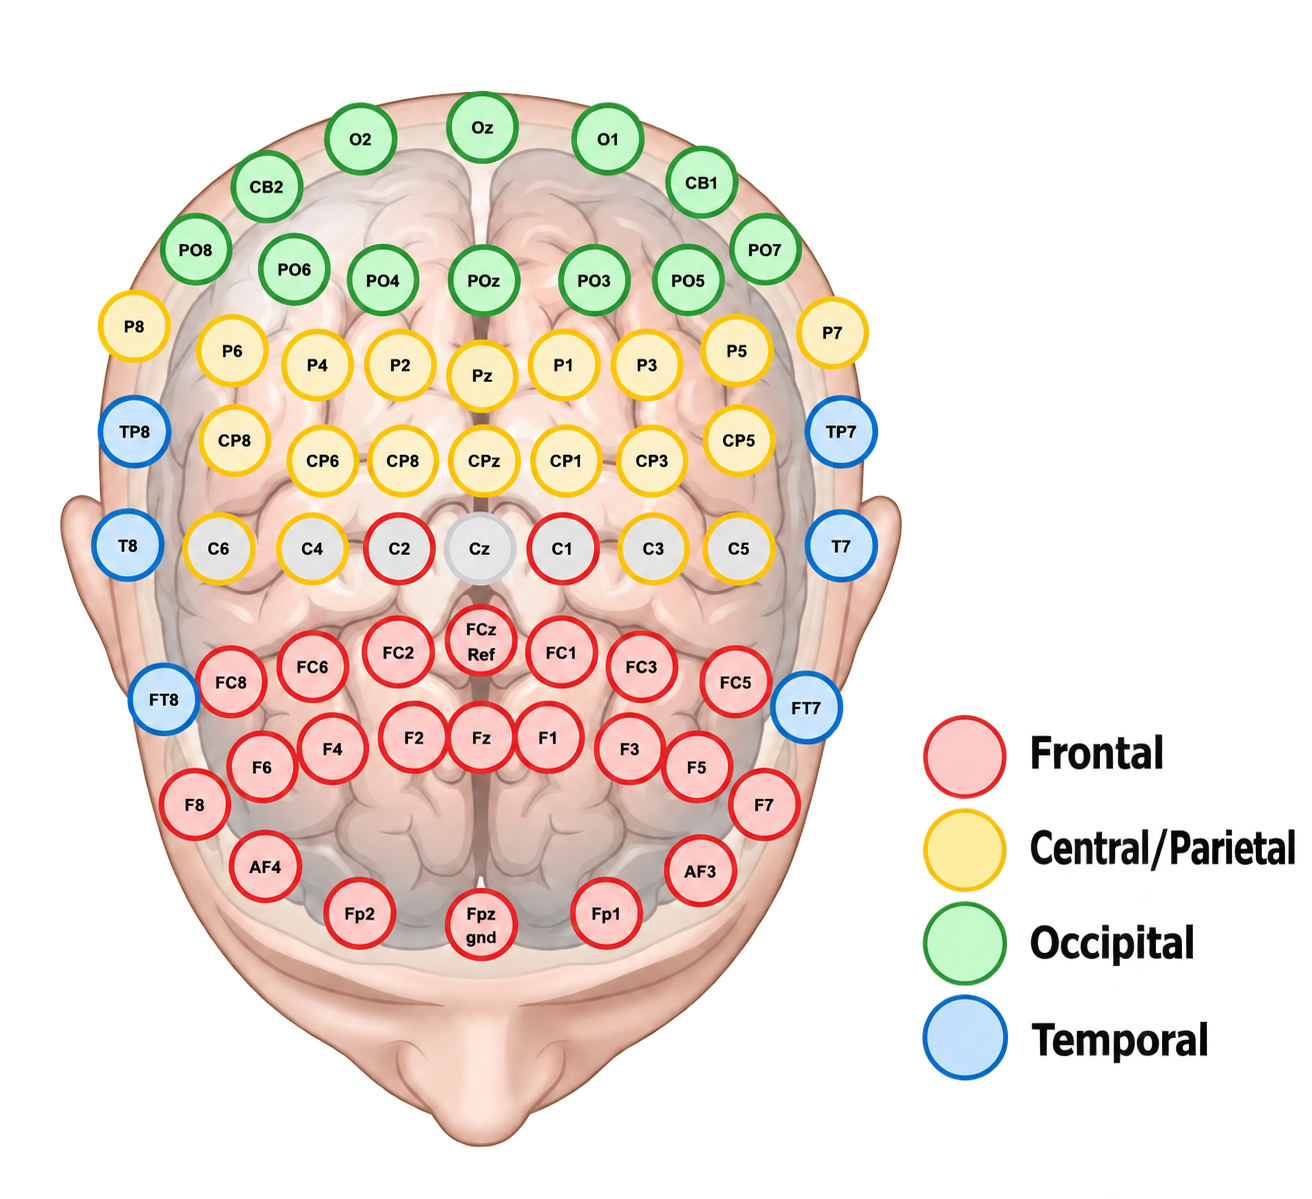
\includegraphics[width=\linewidth]{pictures/Human_Brain_EEG.png}
    \caption{Illustrative multichannel EEG electrode placement across major scalp regions.}
    \label{fig:eeg_electrode_placement}
\end{figure}

Some of these developments involve mobile and wireless systems that allow for more natural recording and bristle and comb-type dry electrodes which reduce the preparation of gel. Reduced-channel setups and cheap devices could increase availability, although the small number of channels, motion artifacts, and unstable electrode contact will continue to be limitations \cite{dadebayev2022commercial}. Real-time processing could help in mobile applications, although modifications in the hardware and recording settings could result in new distribution shifts.

EEG also shows oscillations in delta, theta, alpha, beta, and gamma frequency bands. Examples of these can be seen in Table~\ref{tab:brain_eeg_mapping} and Fig. ~\ref{fig:eeg_frequency_bands}. It is worth mentioning that these waves are not unique to a particular part of the brain and emotions, but depend on the cognitive environment in which they occur.

\begin{table}[t]
    \centering
    \caption{Illustrative distribution of EEG frequency bands across major cerebral regions and their relevance to emotional processing.}
    \label{tab:brain_eeg_mapping}
    \renewcommand{\arraystretch}{1.15}
    \begin{tabularx}{\linewidth}{@{}>{\raggedright\arraybackslash}p{0.31\linewidth}>{\raggedright\arraybackslash}X@{}}
        \hline
        \textbf{Region} & \textbf{Example frequency bands} \\
        \hline

        Frontal &
        Theta (4--7 Hz), beta (13--30 Hz), gamma ($>$30 Hz)
        \cite{nssuha2020eegbased} \\

        \lightrowsep
        Temporal &
        Theta (4--7 Hz), alpha (8--13 Hz), gamma ($>$30 Hz)
        \cite{zhang2023_multifreq_fc_emotion} \\

        \lightrowsep
        Parietal &
        Alpha (8--13 Hz), beta (13--30 Hz)
        \cite{nssuha2020eegbased} \\

        \lightrowsep
        Occipital &
        Alpha (8--13 Hz), beta (13--30 Hz)
        \cite{li2022tutorial} \\

        \lightrowsep
        Central (sensorimotor) &
        Mu (8--13 Hz), beta (13--30 Hz)
        \cite{li2022tutorial} \\

        \lightrowsep
        Limbic-related (indirect) &
        Theta (4--7 Hz), gamma ($>$30 Hz)
        \cite{costa2022aversivememory} \\

        \hline
    \end{tabularx}
\end{table}

\begin{figure*}[t]
    \centering
    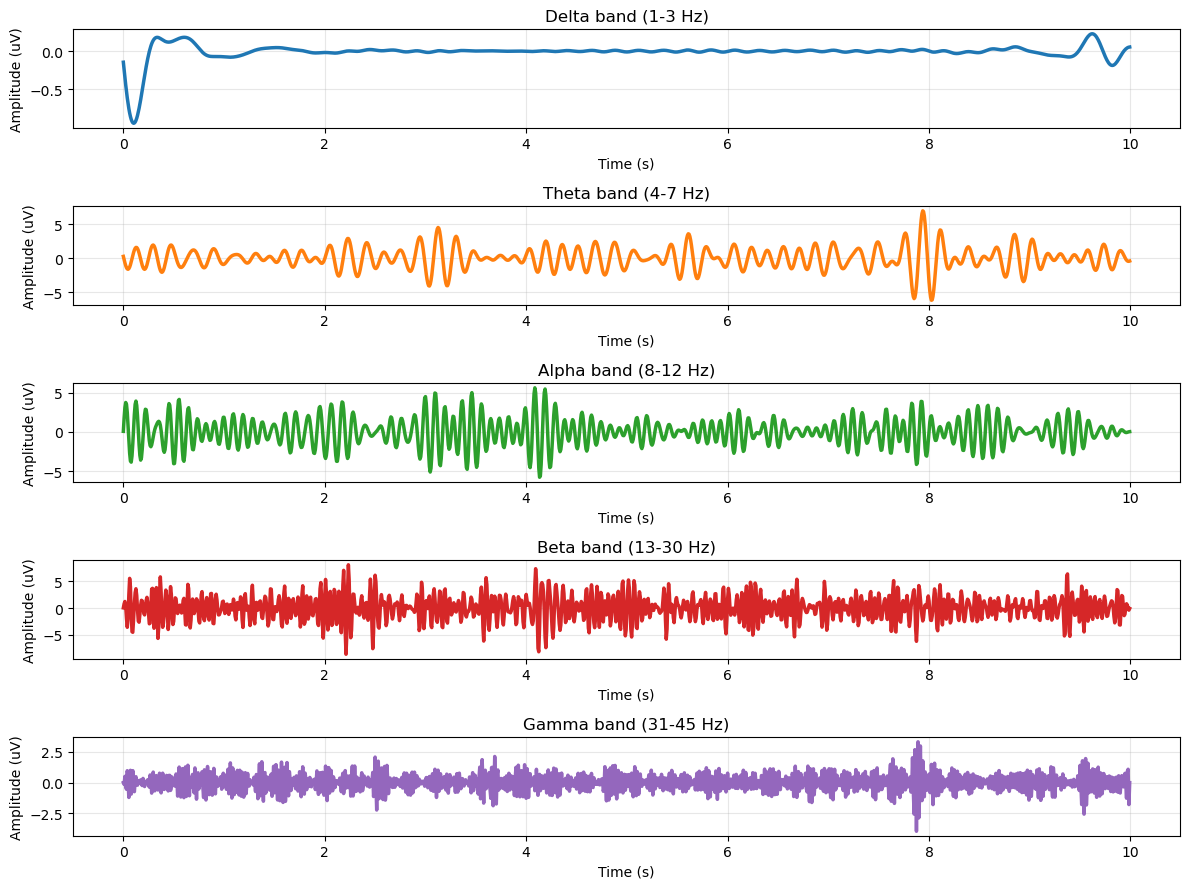
\includegraphics[width=0.8\textwidth]{pictures/Bands.png}
    \caption{Illustrative EEG waveforms across delta (1--3 Hz), theta (4--7 Hz), alpha (8--12 Hz), beta (13--30 Hz), and gamma (31--45 Hz) frequency bands.}
    \label{fig:eeg_frequency_bands}
\end{figure*}

Information regarding regions and bands can be used to extract spatial-spectral features, but standard scalp EEG cannot localize limbic activity. Typically, emotion recognition requires decisions on how to record decisions that ensure the integrity of neural information in light of practical limitations.

\subsection{Multimodal Emotion Modeling}

Emotion modeling in a multimodal framework makes use of behavioral features including facial expression, speech, textual inputs, and gestures along with physiological features including EEG, ECG, EMG, electrodermal activity, and respiration. Different features cover different facets of affective experience and could lessen the reliance on one feature which is inherently prone to noise, ambiguity, or context dependency \cite{soleymani2017survey,baltrusaitis2019multimodal,baltrusaitis2018multimodal}.

In EEG-based emotion recognition, neural measurements provide temporal insights into neural activity, whereas behavioral and physiological measurements provide insights into the expressive or autonomic response. Taken together, these techniques, with their variety in terms of both the timing and type of measurements, could help to gain another view on emotions. The modalities of behavioral and physiological measurements are presented in Fig. ~\ref{fig:modalities}.

\begin{figure*}[t]
    \centering
    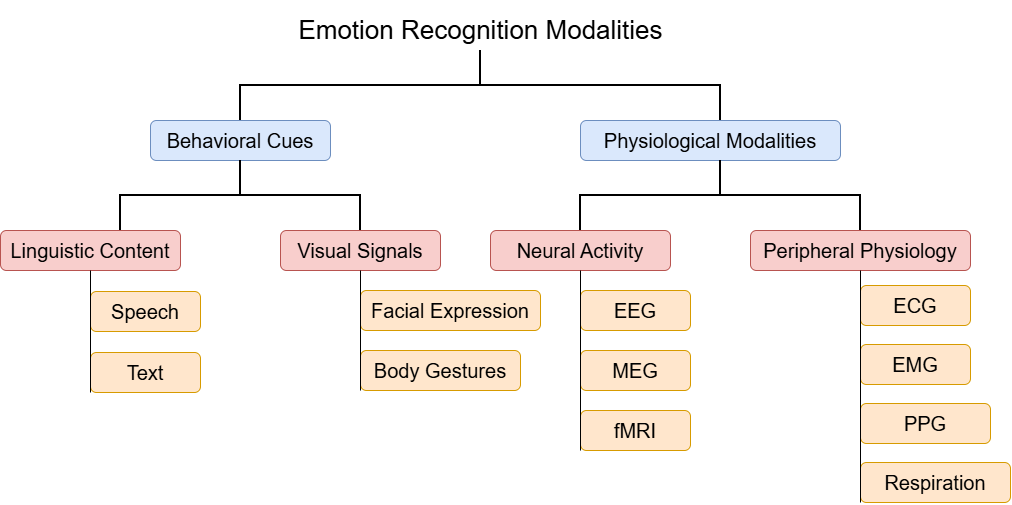
\includegraphics[width=0.75\textwidth]{pictures/Modalities.png}
    \caption{Classification of emotion recognition modalities into behavioral cues and physiological signals, highlighting linguistic, visual, neural, and peripheral physiological measurements.}
    \label{fig:modalities}
\end{figure*}

Multimodal fusion is usually classified into early, intermediate, and late stages of fusion \cite{baltrusaitis2018multimodal}. Early fusion fuses features prior to classification, thus making possible for interaction between modalities but increases dimensions and sensitivity to misalignment \cite{baltrusaitis2019multimodal}. Intermediate fusion provides joint representation, which is able to represent more complicated dependencies but requires higher model complexity \cite{liu2024multimodal}. Late fusion merges output of classifiers for individual modalities, providing modularity but ignoring feature dependencies \cite{liu2024multimodal}. Attention and gating strategies allow for adaptation of the influence of each modality, but the efficiency is conditioned by the quality of the data \cite{mittal2020m3er,rayatdoost2020multimodalgated}.

Multimodal datasets like DEAP and AMIGOS help in studying complementary affective signals \cite{soleymani2017survey,correa2018amigos}. Nevertheless, additional modalities do not guarantee better generalization: synchronization errors, missing signals, inter-subject variability, and computational overhead remain important challenges. Reliable multimodal EEG systems therefore require carefully designed fusion strategies and evaluation against comparable unimodal baselines.
\subsection{EEG Correlates of Emotional States}

Emotion-related EEG activity is reflected in changes across frequency bands, scalp regions, and time rather than in a single waveform amplitude or isolated neural rhythm. This distributed perspective motivates the analysis of oscillatory activity and interactions among brain regions when developing affective representations \cite{chen2025multifrequencyspatial}.

Understanding these correlates is important because emotion-related activity overlaps with broader cognitive processes, including attention and arousal. Modulation of alpha band has been widely studied in affective processing, whereas frontal beta band can provide additional information regarding emotional involvement and regulation, neither is emotion-specific \cite{sun2022atffnet}. Features from the delta and theta frequencies could offer further insights, particularly in the aspect of functional connectivity within varying frequencies \cite{zhang2023_multifreq_fc_emotion}.

Apart from the spectral properties of local signals, the correlations between channels for alpha, beta, and gamma bands can show coordinated brain activity that single channels might be unable to detect \cite{choong2021_corr_alpha_beta_gamma}. Spectral-spatial and connectivity-based models can leverage such correlations to describe the distributed emotional reactions. Time-based models are also important because EEG-based emotions take time to build up and are also dependent on when the stimuli are shown \cite{liu2018_realtime_movie_induced}. Interpretation techniques can be used to test whether discovered patterns are neurophysiologically valid \cite{qing2019_interpretable_eeg_emotion}.

Overall, EEG correlates of emotion are best understood as interacting spectral, spatial, connectivity, and temporal features, rather than unique markers of individual emotions. Combining these two aspects would help in the selection of features and design of the model, however, the validity of these needs to be tested on individual subjects.

\subsection{EEG Signal Processing}

The objective of EEG signal processing in emotion recognition is to transform the raw and noisy EEG signals into representations that are invariant to inter subject and inter session variability, while capturing the neurophysiological dynamics that are relevant to emotion \cite{fdez2021stratified}. In this regard, the signal processing pipeline is equivalent to a series of conditioning steps that include: (i) suppression of non cerebral noises, (ii) standardization of the temporal structure to facilitate learning, and (iii) definition of feature spaces that reveal the temporal, spectral, and spatial characteristics of emotional states. The signal processing pipeline is not just a pre processing step, it is a critical component that determines the information that can be extracted and utilized by the models, and it affects the robustness, interpretability, and generalizability of the models directly \cite{li2022efficientcnncl}.

Affective EEG is usually measured using a specific protocol in which the emotional response is dynamic over time. Therefore, the processing pipeline must accommodate the ability to represent transient responses like, early perceptual responses and sustained responses such as, sustained affective responses. As the datasets move away from the controlled environment, the pipeline focuses more on the resilience of artifacts and stability across domains, encouraging the use of structured denoising, segmentation, and representations that align with the current deep learning encoder models \cite{wang2024dmmr}.


The signals received through an electroencephalogram are known to be quite noisy and prone to a number of artifacts, and therefore preprocessing is an essential step for the recognition of emotions through EEG signals \cite{somers2018mcwfilter}. The preprocessing step is concerned with the cleaning and preprocessing of the raw EEG signals to improve their quality and normalize the input signals for the subsequent steps of feature extraction and classification \cite{erat2024mta}. The preprocessing of EEG signals is an essential step for improving the SNR of EEG signals and removing external noise and artifacts such as power line noise and physiological artifacts such as eye blinks and muscle movements for better performance of the classification model for emotion recognition. It is thus important to apply proper filtering, artifact removal, normalization, and other cleaning procedures before the feature extraction step \cite{ValCalvo2019}. Moreover, the use of similar preprocessing procedures such as the use of similar filters and scaling helps to eliminate variability and errors in the comparison of signals from different domains \cite{wang2024dmmr}. Below, we discuss a variety of critical preprocessing procedures and approaches used in recent studies on EEG based emotion recognition.


\subsubsection{Filtering and Noise Reduction}

The process of filtering and noise reduction is one of the fundamental steps in the preprocessing of EEG signals, in which the raw EEG signals are cleaned of various types of non neural artifacts while keeping the relevant neural components. The EEG signal is very susceptible to external and internal noise, and thus filtering is critical in ensuring that the final signal is indicative of the cognitive or affective processes in the brain instead of other unwanted processes.

The filtering process is of utmost importance in the context of emotion recognition using EEG signals. Emotional states in the brain have very subtle effects in the standard EEG frequency bands, including delta ($\delta$), theta ($\theta$), alpha ($\alpha$), beta ($\beta$), and gamma ($\gamma$). However, these effects can very easily get buried under unwanted effects caused by low frequency drifts (such as skin potentials or sweating), high frequency muscle movements (EMG), or electrical noise such as power line noise.

The noise reduction techniques that are generally used are band pass filtering for restricting the noise band to biologically relevant frequency ranges, notch filtering for eliminating noise components present at particular frequencies such as 50 Hz or 60 Hz, and spatial filtering for reducing the effect of noise artifacts. The more complex noise reduction techniques may include complex filtering methods such as regression analysis for reducing noise artifacts and blind source separation for reducing noise components \cite{Bigirimana2017}. The type of filtering used, i.e., linear filtering, Butterworth filtering, and Chebyshev filtering, is important for avoiding phase distortion of emotional responses.

Even with these techniques, it is difficult to achieve an optimal SNR. The filtering techniques are such that they can eliminate genuine low or high frequency components of brain activity, which are characteristic of emotions. It is therefore critical to properly calibrate and validate filtering techniques to optimize noise reduction while preserving relevant features of the signal.


\subsubsection{Artifact Removal}

Classic filters are unable to completely filter out nonstationary artifacts from the ocular and muscular systems in cases where the frequency band of such artifacts overlaps with that of neural activity. The artifacts from blinking, eye movement, and facial muscle activity can corrupt the EEG data features that will be analyzed for emotion recognition, especially at frontal and temporal electrodes \cite{jiang2019artifactreview}.

\paragraph{Independent Component Analysis (ICA).}
ICA separates multichannel EEG signals into components that correspond to statistically independent sources. The components that are related to the ocular or muscular sources can be recognized from their scalp topographies, time courses, spectra, or additional recordings, and are then discarded when reconstructing the signal. Nevertheless, ICA requires an appropriate source mixing model, and discarding a component that includes both neural and artifact sources may lose important information.

\paragraph{Principal Component Analysis (PCA).}
PCA transforms correlated EEG channels into orthogonal, uncorrelated components ranked by explained variance. Artifact-dominated components can be suppressed before reconstructing the recordings. Although computationally straightforward, PCA separates variance rather than statistically independent sources, consequently, neural and artifactual activity may remain mixed, and rejecting high-variance components can remove relevant brain signals.

\paragraph{Wavelet-Based Artifact Removal.}
Wavelet transforms decompose EEG into time frequency coefficients, allowing transient artifacts to be attenuated through coefficient thresholding and subsequent reconstruction. Adaptive wavelet shrinkage has been investigated for ocular artifact suppression without rejecting entire EEG trials. The efficacy depends on wavelet choice and threshold setting, particularly when there is a temporal and spectral overlap between brain activity and artifact signals.

\paragraph{Hybrid ICA Wavelet Techniques.}
Hybrid methods employ the use of ICA for spatial separation along with wavelet based attenuation of those parts with artifacts. Rather than discarding an entire independent component, wavelet processing can suppress contaminated intervals or coefficients while retaining some underlying neural activity. Automated variants have used statistical measures, including kurtosis and multiscale sample entropy, to identify blink-related components. In an EEG emotion recognition study, hybrid ICA wavelet preprocessing improved classification relative to conventional ICA under the reported experimental conditions. Nevertheless, component selection, wavelet parameters, computational cost, and possible neural signal distortion require careful validation.

Overall, no single method removes every artifact without risk of signal loss. Preprocessing choices should be evaluated for both artifact attenuation and preservation of emotion relevant EEG features, preferably under the same downstream classification protocol.

\subsubsection{Channel Selection and Spatial Filtering}

Channel selection and spatial filtering form part of the basic preprocessing mechanisms that focus on improving signal quality by optimizing the spatial representation of the EEG signal. Rather than considering all channels of the signal, these mechanisms focus on the most important parts of the scalp while avoiding the effects of noisy and irrelevant channels \cite{wang2019channel}. This becomes particularly important when dealing with emotion recognition via EEG signals, where emotion signals tend to be localized and easily obscured by irrelevant neural and physiological activities.

In affective computing, it has been found that the selection of important regions of the brain, particularly those that exhibit emotion, such as the prefrontal and temporal regions, can significantly improve emotion classification \cite{brcfi_valderrama2025}. By selecting a specific subset of the electrodes, it becomes possible to reduce dimensionality, eliminate noisy channels, and simplify the process. Spatial filtering improves the clarity of the signal by re referencing the EEG signal and eliminating global noise components, thus enhancing the signal corresponding to localized neural patterns of emotion.

Several strategies are used in this context. For instance, manual or data driven channel selection methods are used for prioritizing certain electrodes based on neuroscientific knowledge or feature contribution metrics \cite{wang2022hslt}. This ensures that only discriminative channels are used in the process. Spatial filters like CAR and Laplacian filtering are used for reducing reference bias and eliminating common mode noise. These filters are used for normalizing the EEG inputs for different channels and for highlighting spatial gradients that are related to emotional processes.

While these strategies are useful in several ways in terms of reducing computational requirements and improving robustness, they are not without their limitations. For instance, too much reduction of channels in this context would lead to the loss of emotional signals that are spatially distributed. Spatial filters would lead to signal topography distortion if not used properly.


\renewcommand{\arraystretch}{1.2}
\setlength{\tabcolsep}{5pt}
\begin{small}
\begin{table*}[tp]
\centering
\setlength{\tabcolsep}{2pt}
\renewcommand{\arraystretch}{1.07}
\caption{Comparative overview of representative EEG preprocessing techniques relevant to emotion recognition.}
\label{tab:eeg_preprocessing_summary}
\begin{tabular}{
>{\raggedright\arraybackslash}p{0.1196\textwidth}
>{\raggedright\arraybackslash}p{0.1656\textwidth}
>{\raggedright\arraybackslash}p{0.1288\textwidth}
>{\raggedright\arraybackslash}p{0.1656\textwidth}
>{\raggedright\arraybackslash}p{0.1656\textwidth}
>{\raggedright\arraybackslash}p{0.1748\textwidth}
}
\toprule
\textbf{Study} & \textbf{Approach} & \textbf{Preprocessing Method} & \textbf{Advantages} & \textbf{Limitations} & \textbf{Key Findings} \\
\midrule
Somers et al.~\cite{somers2018mcwfilter} & Multi channel Wiener filtering for artifact suppression & Artifact Removal & Preserves neural signal while reducing ocular/muscle noise & Needs covariance estimates; less effective for nonstationary noise & Improves EEG signal quality before emotion decoding \\
\lightrowsep
Kang et al.~\cite{kang2019_ica_aug} & ICA with heuristic artifact aware rejection & Artifact Removal & Effectively isolates and removes major EEG artifacts & Manual component selection may reduce reproducibility & Boosts classification accuracy post cleaning \\
\lightrowsep
Ahmed et al.~\cite{ahmed2023baseline} &
Inverse-filtering-based baseline correction using DEAP EEG recordings &
Filtering and Baseline Normalization &
Reduces baseline-related subject variability and supports subject-independent feature extraction &
Requires baseline recordings; effectiveness depends on baseline estimation and evaluation conditions &
Improved valence and arousal classification compared with conventional subtractive and no-baseline-correction approaches \\
\lightrowsep
Sai et al.~\cite{cysain2018automate} &
Automated artifact classification using SVM and wavelet-ICA &
Hybrid ICA--Wavelet Techniques &
Automatically identifies artifact-contaminated components without manual threshold selection &
Validated primarily for eye-blink artifacts; extension to other artifact types requires further assessment &
Improved identification of artifactual components while largely preserving relevant EEG source signals \\
\lightrowsep
Val Calvo et al.~\cite{ValCalvo2019} & Lightweight real time preprocessing pipeline & Channel Selection and Spatial Filtering & Low latency and computationally efficient & Simplified features limit generalization & Enables real time EEG emotion recognition \\
\lightrowsep
Dura \& Wosiak~\cite{dura2021channelstrategy} & Channel selection strategy to reduce electrodes for deep learning emotion ER & Channel Selection and Spatial Filtering & Reduces channels while retaining discriminative information; lowers computation & Strategy may be dataset/model dependent; risk of losing spatial cues & Shows that careful channel reduction can maintain emotion classification performance \\
\lightrowsep

Issa \& Juhasz~\cite{issa2019wica} &
Selective wavelet-enhanced ICA for ocular artifact removal &
Hybrid ICA--Wavelet Techniques &
Automatic suppression of EOG artifacts while preserving unaffected EEG segments; no reference EOG channel required &
Primarily targets ocular artifacts; depends on accurate identification of contaminated components and intervals &
Improved artifact removal compared with the evaluated component-rejection and wavelet-based methods in both time and spectral domains \\

\bottomrule
\end{tabular}
\end{table*}
\end{small}

Preprocessing methods for EEG have been listed in Table~\ref{tab:eeg_preprocessing_summary}. Traditional techniques for suppressing artifacts, including multichannel Wiener filter, ICA, and wavelet denoising, are mainly aimed at removing the physiological artifacts from the EEG signals without losing the relevant neural data. The ICA and wavelet combination provides more flexibility because it includes both component separation and time frequency analysis. The channel selection and spatial filtering techniques try to eliminate redundant information and increase efficiency of spatial representations. Finally, the real time processing approaches pay special attention to computational effectiveness. According to Table~\ref{tab:eeg_preprocessing_summary}, each of the above mentioned preprocessing approaches includes some compromises between artifacts reduction, preserving emotion neural information, computational complexity, and adaptability. Therefore, the choice of the proper technique should be made taking into account the properties of the recorded signal, experiment protocol, and demands of further emotion recognition models.



The preprocessing of EEG data is the critical first stage that makes up the entire frame of reference and determines whether brain patterns that correspond to emotional states can be simultaneously detected. The drive for affective EEG signatures to be consistently identified relies on a number of factors such as, their low amplitude nature, the amount of ocular, muscular, and nonstationary artifacts present, etc., and as a result, preprocessing conditions, which can either improve or diminish classification accuracy, generalizability, and reproducibility.

The studies presented in Table~\ref{tab:eeg_preprocessing_summary} can be grouped into four complementary categories. Artifact removal strategies, including multi channel Wiener filtering, independent component analysis (ICA) based rejection, and wavelet thresholding have been shown to consistently improve the overall quality of the signal, and also have an impact on downstream recognition, but their applicability involves trade offs such as the validity of the covariance estimated like Gaussian, the subjectivity associated with selecting the appropriate components, or the location of the artifacts being targeted. Hybrid ICA wavelet approaches attempt to merge the separation component of ICA with the time frequency denoising capability of wavelets in order to automate the suppression of ocular artifacts, though the benefits of such techniques may be skewed towards blinks and need to be tested on other sources of artifacts \cite{Bigirimana2017}. Channel selection and spatial filtering strategies like using baseline normalized bandpass filtering, help to mitigate noise and inter subject variability, but rely heavily on the availability of baseline data, and may also attenuate informative bands unintentionally \cite{dura2021channelstrategy}. Lightweight real time pipelines are emphasized to provide low latency and computationally efficient online affective interfaces but not all of the simplifications used in these pipelines are designed to ensure that robustness will be obtained across subjects.


\subsubsection{Feature Extraction}
\label{subsubsec:feature_extraction}

Feature extraction converts preprocessed EEGs into discriminatory features that contain emotion-related brain activity. Given that emotional processes are based on interactions between time, frequency, and space information, combining multiple types of data leads to a more detailed representation of the underlying states. Feature extraction algorithms can generally be classified into hand-crafted representations computed via statistical and signal-processing techniques and learned representations extracted using deep learning systems.

Advances in the design of EEG-based emotion recognition systems nowadays focus more and more on the construction of structured multi-dimensional feature representations that encode relations between channels, time windows, and frequencies. Two-dimensional and three-dimensional feature tensors allow building convolutional models with dependencies between spatial-temporal-spectral data \cite{li2021_3dfeatdfcn}. Recurrent models like Bidirectional Gated Recurrent Units also account for temporal dependencies between consecutive EEG segments \cite{lew2020bigruspatiotemporal}. The same can be done for attention-based models like Conformers and Parallel Transformers--3D CNNs architectures \cite{sun2022paralleltransformer3dcnn}.

Of the conventional feature set, power spectral density (PSD) and differential entropy (DE) still continue to be popular for frequency-specific EEG activity characterization \cite{chen2019feature}. While PSD captures signal power in specific frequency ranges, DE represents a logarithmic value of signal variance when a Gaussian assumption holds. For a Gaussian EEG segment, differential entropy can be defined as
\begin{equation}
    h(X) = \frac{1}{2}\ln\left(2\pi e\sigma_X^2\right),
    \label{eq:feature_de}
\end{equation}
where $\sigma_X^2$ denotes the variance of the EEG signal. In this case, DE is linearly dependent on logarithmic power of signal, representing a concise form of emotion classification. Despite the fact that PSD and DE are relatively computationally convenient spectral parameters, temporal averaging may obscure the short-lived neural processes. However, both methods require correct setting of window length and overlap \cite{brcfi_ma2025sfswts}.

Overall, EEG feature extraction has progressed from handcrafted signal descriptors toward learned multidimensional representations capable of capturing interactions across neural domains. Nevertheless, their effectiveness depends on preserving emotion-discriminative information while controlling feature redundancy, computational complexity, and sensitivity to recording variability. The following subsections discuss temporal, spectral, spatial, and multidomain feature extraction strategies in greater detail.


\paragraph{Temporal Domain Features}

Temporal domain features play a critical role in emotion recognition systems that use EEG as a medium, as emotions are dynamic experiences that change over time \cite{abgeena2023slstmatt}. Emotions are dynamic experiences that change over time and are often composed of a series of neural events that can't be described by time independent features. Temporal features help the emotion recognition system understand how brain activity is changing over time as a response to an emotional stimulus. These features are critical in handling intersubject variability in the timing of the emotion recognition response, as they help the system concentrate on the timing of the signal rather than relying on synchronous stimuli and labels.

Within the emotion decoding paradigm, temporal modeling has been integrated using a variety of deep learning approaches that have taken advantage of the strengths of sequence learning. As an example, recurrent models such as LSTMs or bidirectional RNNs have been widely used to capture the dependencies between successive segments of the EEG signals, modeling the temporal dynamics of affective states \cite{shen20204dcrnn}. In other instances, hybrid models have been proposed that take advantage of the strengths of both convolutional and recurrent models to learn the spatial patterns and their temporal dynamics \cite{yang2018pcrnn,xu2023gruconv}. In addition, hierarchical sequence models have been proposed that learn the signals regionally and then aggregate them globally, thus preserving the spatial patterns while modeling the temporal dynamics \cite{li2019regionaltoglobal}. Finally, temporal convolutional models have been proposed that offer an alternative to recurrent models, enabling the modeling of long range dependencies using hierarchical, dilated convolutional architectures \cite{yang2024ftcn}.

Although these methods are useful in terms of the recognition of dynamic patterns of emotion, there are challenges that are associated with these methods. These challenges include difficulties in integrating frequency and spatial information or the use of uniform timing \cite{li2022mvsstma}. The selection of appropriate window length and temporal resolution is also important in temporal domain modeling \cite{yin2021gcnlstm}. This is important for the avoidance of overfitting or the loss of relevant information, particularly for the improvement of the performance of emotion recognition, especially for naturalistic or continuous emotional scenarios where there is the presence of individual variations of emotional expression timing \cite{nath2020lstm}.


\paragraph{Frequency Domain Features}
Frequency domain features provide a promising approach for analysing the rhythmic characteristics of EEG signals, which are closely associated with emotional processing in the human brain. These features enable researchers to examine the distribution of EEG signal power across standard frequency bands, including theta, alpha, beta, and gamma, whose oscillatory activities have been investigated in relation to different emotional states. Unlike raw time domain representations, frequency domain features provide a compact description of neural oscillatory activity within a given analysis window. However, their stability across recording sessions and subjects depends on signal preprocessing, recording conditions, and inter individual variability \cite{zhang2024bfenet}.

Frequency domain features are particularly important in EEG based emotion recognition because they enable the analysis of band specific neural activity associated with emotional processes. For example, changes in beta band activity have been associated with heightened arousal, while frontal alpha power asymmetry has been investigated in relation to affective valence and hemispheric differences in emotional processing. Although spectral power features may be less sensitive to small temporal shifts than raw waveform representations, they remain susceptible to noise, physiological artifacts, and variations in spectral estimation parameters. Nevertheless, appropriate filtering and spectral feature extraction can provide informative representations for developing EEG based emotion recognition models.

Several methodologies have been explored for the effective modeling of frequency domain features. For instance, in some methodologies, the EEG signals were converted into spectrograms using various tools such as the STFT, allowing deep learning models to effectively learn the relative contribution of frequency domain features~\cite{zheng2022multi}. In other methodologies, the band power and differential entropy were considered as feature inputs, allowing the model to effectively capture the spectral content of each channel. More recent methodologies have also been explored, allowing the model to effectively capture the spectral relationship between channels using tools such as the convolutional model and attention mechanism~\cite{song2022eegconformer}. In addition, multi domain models have also been explored, allowing the model to integrate frequency domain and temporal domain representations for improved emotion recognition accuracy~\cite{li2021multidomain}.

However, frequency domain modeling for emotion detection with its emphasis on consistent rhythmic patterns has its own set of limitations. For example, there is a need for balance in terms of spectral resolution and computational efficiency. In addition, the parameters of transformations such as STFT are critical and may affect the overall model. Moreover, frequency domain modeling may not account for other dynamics that are critical in decoding complex emotion responses.

In summary, frequency domain features form an essential pillar in EEG based emotion recognition systems. They are reliable and highly correlated with other emotion related features. In addition, frequency domain modeling with other domains forms an essential tool in modeling complex affective states with neurophysiological meaning~\cite{li2021multidomain,zheng2022multi}.



\paragraph{Temporal Frequency Domain Features}

Frequency domain features are the core of emotion recognition using EEG, as they are based on the rhythmic patterns of the brain's electrical activity, which are directly related to emotional states. The rhythmic patterns of the electrical signals in certain bands of frequencies, such as the delta band (1-4 Hz), the theta band (4-8 Hz), the alpha band (8-13 Hz), the beta band (13-30 Hz), and the gamma band (30-50+ Hz), are known to relate to various aspects of emotion. For instance, the power of alpha and beta rhythms is known to relate to the level of arousal and the valence of emotion. The asymmetry of alpha power in the frontal region is known to relate to approach/withdrawal aspects of emotion \cite{cui2020regionalasymcnn}. Frequency specific modulations are generally consistent across subjects and sessions, and hence are useful indicators of emotion classification.

In practice, the analysis of the electrical signals in the frequency domain is achieved through various techniques such as the Fourier transform, the wavelet transform, and the differential entropy method. The above techniques are used to transform the raw electrical signals to a more compact representation. The compact representation is useful because the electrical signals are more susceptible to noise.

Recently, various modeling techniques have adopted frequency domain features in different ways. In some models, frequency domain feature extraction has been performed independently, and the extracted features have been combined with temporal or spatial features to obtain enhanced emotion specific information. In other models, convolutional or attention based encoders have been employed to extract frequency domain features, which have been treated similarly to visual inputs to learn abstract frequency domain representations \cite{hwang2020_decnn,liu2025_dssanet}. In addition, various models have utilized graph based reasoning to extract frequency domain feature encoded nodes to identify inter band relationships and regional patterns \cite{tian2025accnet}.

Even though frequency domain based models have shown promising performance, various trade offs have been identified in their performance, including sensitivity to the parameters of the decomposition and windowing techniques employed in the models \cite{gupta2019fawt}. In addition, models that have adopted frequency domain based features may overlook essential temporal patterns, thus failing to accommodate different subjects with varying frequency domain patterns. Nonetheless, frequency domain based features have shown promising performance when combined with other features to provide robust brain state oscillatory patterns and improve emotion recognition systems.


\paragraph{Integration and Fusion Strategies Across Feature Domains}
The integration of temporal, frequency, and spatial features has emerged as a primary concern in EEG based emotion recognition, owing to the multidimensional nature of emotional brain responses. These features describe emotional responses from different but complementary perspectives, where temporal features describe the dynamics of brain responses, frequency features describe brain responses in terms of oscillatory properties, and spatial features describe brain responses in terms of brain regions \cite{arnau2017_energy_connectivity_fusion}. Emotion expression in the brain does not occur in individual channels or frequency bands but occurs through interactions across multiple brain responses. Therefore, brain responses that combine multiple views are more expressive and tend to generalize better across subjects and sessions \cite{liu2024dacapsnet}.

The importance of multi domain fusion becomes critical when handling noisy or uncertain EEG signals. There are scenarios where one domain may not contribute much or may be noisy, such as noisy temporal responses owing to movement, but brain responses in other domains can serve as a fallback, ensuring that fusion based methods are more robust, especially when handling real world or cross subject scenarios.

However, recent developments in multi domain fusion architectures have focused on flexibility and adaptability. Many of these methods involve multi branch architectures in which domain specific feature extractors process temporal, spectral, and spatial information in parallel, followed by fusion layers that combine the features. Some of these methods involve graph convolutional networks (GCNs) to represent spatial relationships between EEG channels, combined with temporal frequency encoders. Others involve attention mechanisms to dynamically assign weights to features across domains according to their relevance to the emotional state \cite{tao2020channelselfatt}.

There is also an emerging trend towards deeper architectures that learn their own fusion policies implicitly. These include transformer based feature encoders with domain specific attention mechanisms and approaches with masked modeling for cross domain reconstruction \cite{li2022mvsstma}. These are very powerful architectures. However, they tend to be computationally expensive, requiring significant memory and regularization during training to avoid overfitting. Moreover, they also present difficulties with regards to their interpretation, as it is not clear what contribution each of the different domains makes towards the overall emotion prediction.

To summarize, the integration of various EEG domains can improve the model’s ability to learn discriminative and generalizable representations of emotions. Fusion techniques can provide better modeling of emotional patterns, handling of noise, and stability of cross subject models. Although the above techniques provide considerable benefits, the trade off needs to be managed for the handling of computational complexities and the interpretability of the models. It is believed that future research will concentrate on the development of more lightweight, interpretable, and data efficient fusion techniques that can provide the benefits of multi domain integration.applications.


Each of these features provides supplementary information for emotion recognition from EEG, and their combination can contribute to stronger and more accurate emotion recognition models. Temporal features reflect the dynamic nature of emotional responses and their variation. Emotions are processes that depend on time. For example, emotional arousal may increase and subsequently decrease over time \cite{zhu2022gatstpl}. Frequency features focus on specific frequency bands of neurophysiological responses that are related to emotional processes. For example, changes in alpha and beta band power have been associated with relaxation and heightened cognitive engagement, respectively. Spatial features reflect emotional processes across different brain regions. For example, frontal alpha asymmetry has been investigated as an indicator of affective valence and hemispheric differences in emotional processing \cite{cui2020regionalasymcnn}. These three aspects are complementary, and their combination can compensate for some of the limitations associated with individual feature types. Empirical studies have demonstrated that integrating information from multiple feature domains, particularly spatial information with temporal or spectral representations, can improve emotion recognition performance compared with approaches relying on individual representations. In particular, spatial features are often combined with temporal or frequency features to provide context about where in the brain particular temporal or spectral patterns occur. The combination of features from multiple domains therefore creates a more comprehensive representation of the EEG signal, which can potentially improve the accuracy and robustness of emotion recognition against noise and inter individual variation.

Fusion is achieved using various architectural styles. First, tensor fusion involves the creation of multi dimensional input representations like, 3D tensors that enable an encoder network to learn interaction patterns implicitly. Second, multi branch fusion involves the use of dedicated encoders for each domain of temporal, spectral, and spatial and subsequent fusion of intermediate representations. Third, attention based fusion leverages adaptive weightings that highlight the most relevant domain or channel representations depending on varying noise conditions. The use of a dual branch dynamic graph convolution and adaptive transformer fusion presents an example of the potential for using spatial reasoning and attention based fusion mechanisms that leverage inter channel relationships and remain adaptive in feature weightings \cite{sun2022atffnet}. For multi domain EEG encodings, transformer networks are also developed that take in representations from various feature spaces and learn to fuse these using self attention \cite{sun2023meegtransformer}.



\begin{small}
\begin{table*}[tp]
\centering
\setlength{\tabcolsep}{2pt}
\renewcommand{\arraystretch}{1.07}
\caption{ Comparative overview of representative EEG feature extraction methods for emotion recognition.}
\label{tab:eeg_feature_extraction_summary}
\begin{tabular}{
>{\raggedright\arraybackslash}p{0.1196\textwidth}
>{\raggedright\arraybackslash}p{0.1840\textwidth}
>{\raggedright\arraybackslash}p{0.1104\textwidth}
>{\raggedright\arraybackslash}p{0.1656\textwidth}
>{\raggedright\arraybackslash}p{0.1656\textwidth}
>{\raggedright\arraybackslash}p{0.1748\textwidth}
}
\toprule
\textbf{Study} &
\textbf{Approach} &
\textbf{Domain Category} &
\textbf{Advantages} &
\textbf{Limitations} &
\textbf{Key Findings} \\
\midrule

Li et al.~\cite{li2021_3dfeatdfcn} &
3D spatial temporal spectral features with FCNs &
Spatial-Temporal-Spectral &
Combines rich domain information in unified volume &
Heavier computation than 2D encodings &
Improves accuracy across datasets \\

\lightrowsep

Lew et al.~\cite{lew2020bigruspatiotemporal} &
Spatiotemporal encoding with Bi-GRU &
Spatial-Temporal &
Captures evolving emotion responses &
Sensitive to segmentation granularity &
Better for gradual emotion transitions \\

\lightrowsep

Song et al.~\cite{song2022eegconformer} &
Conformer model for EEG sequences &
Spatial-Temporal &
Fuses local and global patterns effectively &
Can overfit without regularization &
Outperforms traditional CNN/RNN models \\

\lightrowsep

Jia et al.~\cite{jia2020sstemotionnet} &
3D DenseNet with attention across domains &
Spatial-Temporal-Spectral &
Learns dynamic relevance between features &
Model complexity is high &
Salient EEG areas enhance emotion decoding \\

\lightrowsep

Sun et al.~\cite{sun2022paralleltransformer3dcnn} &
Parallel transformer + 3D CNN fusion &
Spatial-Temporal &
Separates local/global representation branches &
Careful tuning required for balance &
Shows strong performance on multi channel inputs \\

\lightrowsep

Yudhana et al.~\cite{yudhana2020human} &
FFT based spectral features with $k$NN classifier &
Spectral &
Simple and computationally efficient &
Ignores temporal dynamics; limited scalability &
Shows the viability of classic frequency features \\

\lightrowsep

Chen et al.~\cite{chen2019feature} &
Differential entropy features with LDA projection &
Spectral &
Compact and discriminative spectral representation &
Linear assumptions limit expressiveness &
Improves valence and arousal classification \\

\lightrowsep

Bigirimana et al.~\cite{bigirimana2020emotion} &
Multi class CSP spatial filtering &
Spatial &
Enhances emotion specific spatial patterns &
Sensitive to non stationarity and subject variation &
Boosts multi class EEG emotion accuracy \\

\lightrowsep

Lin et al.~\cite{lin2010eegpower} &
Power spectral asymmetry analysis for emotion classification &
Frequency &
Captures hemispheric imbalance related to valence &
Sensitive to noise and baseline drift &
Demonstrates frontal alpha asymmetry correlates with emotional valence \\

\lightrowsep

Jenke et al.~\cite{jenke2014feature} &
Comparative evaluation of frequency domain EEG features &
Frequency &
Identifies robust spectral descriptors for emotion decoding &
Requires feature selection optimization &
Highlights differential entropy and PSD as strong frequency predictors \\

\lightrowsep

Murugappan et al.~\cite{murugappan2010time} &
Statistical time domain features for emotion classification &
Temporal &
Low computational cost; suitable for real time systems &
Limited ability to capture nonstationary dynamics &
Shows time domain variance and mean features discriminate emotions \\

\lightrowsep

Gupta et al.~\cite{gupta2019temporal} &
Hjorth parameters and higher order statistics &
Temporal &
Reflects signal activity and mobility characteristics &
Sensitive to artifacts &
Demonstrates temporal descriptors contribute to valence arousal recognition \\

\lightrowsep

Petrantonakis \& Hadjileontiadis~\cite{petrantonakis2010emotion} &
Higher order crossings (HOC) for EEG temporal dynamics &
Temporal &
Captures nonlinear signal characteristics &
Requires careful parameter tuning &
HOC features enhance multi class emotion accuracy \\

\lightrowsep

Zhao et al.~\cite{zhao2019stft} &
Short Time Fourier Transform for emotional EEG analysis &
Temporal Frequency &
Preserves both temporal and spectral information &
Window size selection impacts performance &
STFT based representations improve arousal classification \\

\lightrowsep

Subasi \& Gursoy~\cite{subasi2010wavelet} &
Wavelet transform for EEG emotional state detection &
Temporal Frequency &
Handles non stationary EEG signals effectively &
Higher computational complexity &
Wavelet coefficients improve emotional discrimination \\
\lightrowsep

Al Nafjan et al.~\cite{alnafjan2017psd} &
PSD based spectral feature extraction with SVM &
Frequency &
Simple and computationally efficient &
Limited temporal resolution &
Confirms spectral power variations distinguish valence states \\

\midrule
\multicolumn{6}{r}{\textit{Continued on next page}} \\
\bottomrule

\end{tabular}
\end{table*}
\end{small}


\begin{small}
\begin{table*}[tp]
\centering
\setlength{\tabcolsep}{2pt}
\renewcommand{\arraystretch}{1.07}

\addtocounter{table}{-1}

\caption{ Comparative overview of representative EEG feature extraction methods for emotion recognition.}

\begin{tabular}{
>{\raggedright\arraybackslash}p{0.1196\textwidth}
>{\raggedright\arraybackslash}p{0.1840\textwidth}
>{\raggedright\arraybackslash}p{0.1104\textwidth}
>{\raggedright\arraybackslash}p{0.1656\textwidth}
>{\raggedright\arraybackslash}p{0.1656\textwidth}
>{\raggedright\arraybackslash}p{0.1748\textwidth}
}
\toprule
\textbf{Study} &
\textbf{Approach} &
\textbf{Domain Category} &
\textbf{Advantages} &
\textbf{Limitations} &
\textbf{Key Findings} \\
\midrule

Li et al.~\cite{li2018fusion} &
Feature level fusion of spatial and spectral EEG descriptors &
Fusion &
Integrates complementary information &
Risk of high dimensionality &
Fusion improves robustness across subjects \\

\lightrowsep

Zheng \& Lu~\cite{zheng2015investigating} &
Combined frequency and spatial asymmetry features &
Fusion &
Exploits hemispheric asymmetry and band power &
Requires careful channel selection &
Identifies critical bands and regions for emotion decoding \\

\lightrowsep

Zhang et al.~\cite{zhang2020multifeature} &
Multi feature fusion with deep neural networks &
Fusion &
Learns hierarchical representation from heterogeneous features &
High model complexity &
Feature fusion enhances cross subject generalization \\

\bottomrule
\end{tabular}
\end{table*}
\end{small}


A comparative overview of representative EEG feature extraction techniques is presented in Table~\ref{tab:eeg_feature_extraction_summary}, illustrating the methodological progression from conventional signal descriptors to deep learning based multi domain representations. Traditional temporal and frequency domain approaches, including statistical measures, higher order crossings, power spectral analysis, and differential entropy, provide relatively compact descriptions of emotion related EEG activity. Time frequency techniques, such as short time Fourier analysis, wavelet decomposition, and the Hilbert  Huang transform, extend these representations by examining how spectral characteristics evolve over time. Spatial feature extraction approaches, including common spatial patterns, focus on the distribution of neural activity across electrodes. More recent learning based methods integrate multiple feature domains through convolutional, recurrent, graph based, and attention driven architectures, allowing complementary information to be combined within a unified representation. As highlighted in Table~\ref{tab:eeg_feature_extraction_summary}, these approaches involve different trade offs between computational efficiency, representation capacity, temporal sensitivity, and model complexity. Although multi domain learning can offer a richer description of affective neural activity, its effectiveness depends on the selected feature representations, fusion strategy, and experimental evaluation protocol. Therefore, appropriate feature extraction should balance discriminative performance with computational requirements, interpretability, and robustness across recording conditions.


\subsubsection{Feature Selection}
In emotion recognition datasets using electroencephalogram (EEG) signals, datasets contain high dimensional feature vectors, including a high number of channels as well as different frequency band features. At the same time, several datasets contain a relatively low number of instances compared to the high dimensionality of the dataset. As a result, there is a great tendency for the occurrence of the curse of dimensionality, which may cause models to overfit as well as possibly ignore several relevant features in the dataset, which often reduces model efficiency as well as generalization of the classifier. Feature selection is one of the main concepts in pattern recognition as well as machine learning that helps reduce a high number of features in a dataset, containing only the most efficient as well as unique features, which can help in improving the efficiency of a classifier in pattern recognition as well as in improving the efficiency of the machines used~\cite{hamzah2024heliyon}.

\paragraph{Filter Methods}
Filter based feature selection is one of the most used feature selection techniques in EEG based emotion recognition systems. This is mainly because of its relative ease of implementation, speed, and classifier agnostic nature. Filter based feature selection approaches attempt to measure the significance of the features before actually training a classifier. Hence, these are generally employed as a pre processing step of the machine learning pipeline to reduce dimensionality and improve the learning efficiency of downstream classifiers.

The relevance of the filter method is determined by the nature of EEG data, which is usually characterized as being both high dimensional and noisy in nature. There is usually an involvement of emotion related features as well as other features in a pool of redundant and irrelevant information. Filtering out these less informative features at an early stage enables filter approaches to build better classification performance, reduce overfitting, and improve interpretability. This is particularly significant for EEG based emotion recognition tasks.

There are many different filter based methods for selecting good features. Two examples of filter selection methods are correlation based selection and mutual information (MI) selection. A correlation based method examines the correlation between each feature and the emotional label it is related to in order to find all of the features that have a high correlation with the individual emotional labels and the overall target emotion label \cite{Chakladar2018}. In an MI based method, the MI score of each feature is calculated with respect to the associated target label as well as with respect to all other features, to assess the relevance and redundancy of each feature. Similarly, each feature in the mRMR framework is evaluated based on its MI to the target label as well as its MI compared to all other features. The purpose of the mRMR framework is to identify a small, non redundant collection of features that provide the most information when identifying emotion labels. Extensions of the mRMR framework have been developed that incorporate methods such as sequential forward search or floating search, allowing for a larger, more exhaustive search of the feature space with improved efficiency.

Filter based methods have certain inherent limitations, they may produce suboptimal subsets of features when there are emotional patterns throughout multiple feature combinations or only when comparing each feature separately and independently. Therefore, the subset of features determined by filter methods will not always correspond to an optimal decision boundary that a classifier might find in an EEG based emotion recognition system, and so may lead to poor classification performance when classifiers use the features selected from the filter methods. However, filter methods remain viable techniques for EEG emotion recognition systems because of their large scale ability to apply to general tasks and their ability to be generalized \cite{yin2020lrfs}.


\paragraph{Wrapper Methods}

Wrapper techniques make use of an elected classifier to estimate the performance of EEG feature subset selections, whereas filter techniques assess the features based on selection criteria that are unrelated to the classifier. Wrapper techniques can account for interactions among temporal, spectral, and spatial EEG features, but at the expense of increased computational overhead due to repeated model building \cite{brcfi_nakisa2018}.

Representative approaches include recursive feature elimination (RFE), which iteratively removes features according to their importance in a fitted model, and evolutionary algorithms that search candidate subsets through operations such as mutation and selection. Evolutionary feature and channel selection has been investigated for EEG emotion recognition, including mobile recordings, differential-evolution-based selection has also been evaluated for subject-independent emotion classification \cite{brcfi_kannadasan2023}.

Despite their flexibility, wrapper methods can overfit the data used to select features and may be impractical when each candidate subset requires expensive training. Feature selection should therefore occur strictly within the training partitions, with separate or nested validation used for performance estimation. Ultimately, the value of wrapper selection depends on its computational efficiency and demonstrated performance on genuinely unseen subjects or recording sessions, rather than improvement on the feature-selection data alone.

\renewcommand{\arraystretch}{1.2}
\setlength{\tabcolsep}{5pt}
\begin{small}
\begin{table*}[tp]
\centering
\setlength{\tabcolsep}{2pt}
\renewcommand{\arraystretch}{1.07}
\caption{ Comparative overview of representative filter-based, wrapper-based, and embedded feature selection techniques relevant to EEG emotion recognition.}
\label{tab:eeg_feature_selection_summary}
\begin{tabular}{
>{\raggedright\arraybackslash}p{0.1196\textwidth}
>{\raggedright\arraybackslash}p{0.1840\textwidth}
>{\raggedright\arraybackslash}p{0.1104\textwidth}
>{\raggedright\arraybackslash}p{0.1656\textwidth}
>{\raggedright\arraybackslash}p{0.1656\textwidth}
>{\raggedright\arraybackslash}p{0.1748\textwidth}
}
\toprule
\textbf{Study} & \textbf{Approach} & \textbf{Feature Selection Method} & \textbf{Advantages} & \textbf{Limitations} & \textbf{Key Findings} \\
\midrule
Xu et al.~\cite{xu2021_pairwise_redundancy} & Orthogonal regression for pairwise redundancy reduction & Embedded & Removes overlapping features, boosts relevance & Assumes linearity in correlations & Improves generalization across individuals \\
\lightrowsep
Kannadasan et al.~\cite{kannadasan2023_de_eeg} & Differential evolution for feature subset selection & Wrapper & Searches compact, accurate feature sets & Evolution search is slow at scale & Increases classification stability in DEAP \\

\lightrowsep
Liu et al.~\cite{liu2018emdfeature} & EMD with optimal subset evaluation & Wrapper & Efficient combination of decomposition and selection & EMD results vary with input noise & Smaller feature sets yield higher accuracy \\

\lightrowsep
Wang et al.~\cite{wang2019channel} & NMI based EEG channel selection & Filter & Reduces redundancy and sensor count & Subset may vary across subjects & Preserves accuracy with fewer channels \\

\lightrowsep

Al Nafjan et al.~\cite{alnafjan2017psd} & ReliefF based statistical feature ranking & Filter & Fast computation and noise tolerant ranking & May overlook nonlinear inter feature interactions & Demonstrates effective dimensionality reduction for valence classification \\
\lightrowsep

Jenke et al.~\cite{jenke2014feature} & Comparative evaluation of filter based feature ranking methods & Filter & Identifies most discriminative EEG descriptors & Dependent on classifier compatibility & Highlights mutual information and Fisher score as effective EEG selectors \\
\lightrowsep

Shen et al.~\cite{shen2010feature} & Sequential forward selection with SVM evaluation & Wrapper & Produces compact feature subsets & Greedy search may miss global optimum & Reduces dimensionality while preserving classification performance \\

Zhang et al.~\cite{zhang2016lasso} & LASSO based sparse feature learning & Embedded & Automatically enforces sparsity during training & Linear constraint limits nonlinear capture & Sparse modeling enhances cross subject stability \\
\lightrowsep

Li et al.~\cite{li2019embedded} & Deep neural network with attention based embedded selection & Embedded & Learns task relevant features automatically & Requires large training data & Embedded attention improves discriminative EEG feature learning \\
\bottomrule
\end{tabular}
\end{table*}
\end{small}

A comparative overview of representative EEG feature selection techniques is presented in Table~\ref{tab:eeg_feature_selection_summary}, highlighting the methodological differences, advantages, and limitations of filter based, wrapper based, and embedded approaches. Filter based methods primarily evaluate statistical relationships between individual features and emotion labels using criteria such as mutual information, normalized mutual information, and minimum redundancy maximum relevance (mRMR). These methods offer relatively low computational complexity and can reduce redundant information without depending on a particular classification algorithm. In contrast, wrapper based approaches employ iterative feature subset evaluation through evolutionary optimization, genetic algorithms, or sequential search strategies, allowing the selection process to account for interactions between features and classifier performance. However, their repeated model evaluations introduce additional computational costs and potential overfitting risks. Embedded methods integrate feature selection into the model development process through sparse learning, model dependent feature ranking, or attention based mechanisms, enabling the simultaneous optimization of feature relevance and predictive representations. As summarized in Table~\ref{tab:eeg_feature_selection_summary}, each category presents different trade offs between computational efficiency, feature redundancy reduction, classification performance, and model interpretability. Consequently, selecting an appropriate feature selection strategy requires careful consideration of EEG dimensionality, dataset characteristics, computational resources, and subject dependent or subject independent evaluation protocols. These considerations are particularly important for developing reliable EEG based emotion recognition systems capable of maintaining discriminative performance across individuals and recording conditions.

Across all categories, a consistent finding is that reducing irrelevant or overlapping EEG features enhances generalization, improves robustness across subjects, and lowers computational burden without sacrificing accuracy. The table therefore reflects a broader research trend toward compact, discriminative, and task adaptive feature representations, which are essential for scalable and cross subject emotion recognition systems.

\begin{figure*}[htb]
    \centering
    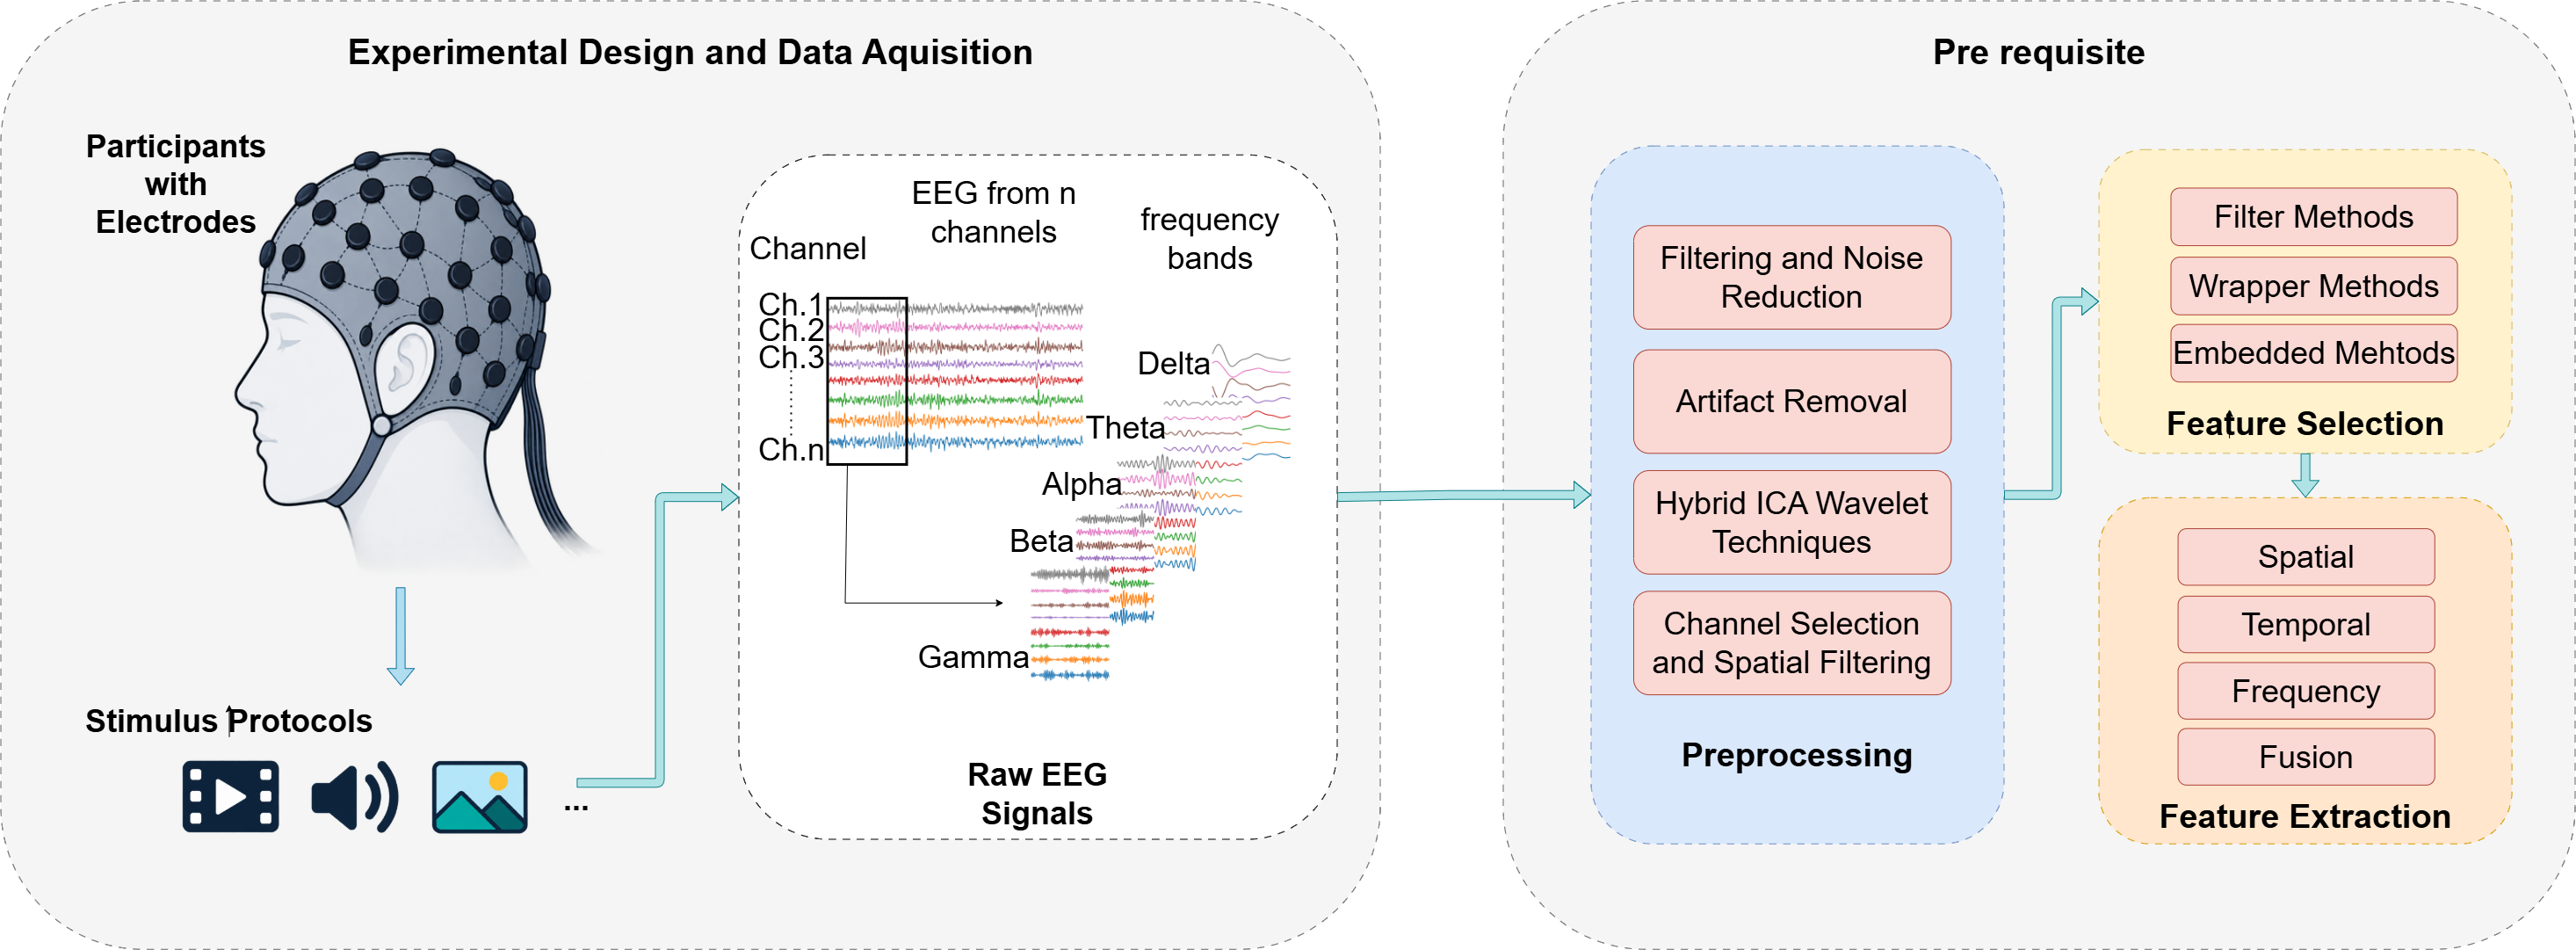
\includegraphics[width=\linewidth]{pictures/Method Overview.png}
    \caption{Overview of the experimental design, EEG data acquisition, and signal processing stages for emotion recognition.}
    \label{fig:eeg_method_overview}
\end{figure*}


Fig. ~\ref{fig:eeg_method_overview} illustrates the principal stages involved in acquiring and preparing EEG signals for emotion recognition. The process begins with experimental protocols in which participants are exposed to emotion eliciting stimuli, such as videos, audio recordings, and images, while their neural responses are captured through multichannel EEG electrodes. The acquired signals contain time varying neural activity distributed across conventional frequency bands, including delta, theta, alpha, beta, and gamma. However, raw EEG recordings are susceptible to physiological artifacts, environmental interference, and irrelevant signal components, making appropriate preprocessing essential before extracting emotion related information. Common procedures include noise filtering, artifact removal, independent component analysis (ICA), wavelet based denoising, and spatial filtering. Following preprocessing, temporal, frequency domain, and spatial features can be extracted individually or combined through feature fusion to characterize complementary aspects of affective neural activity. Feature selection techniques, including filter, wrapper, and embedded approaches, can subsequently be employed to identify informative representations and reduce feature redundancy. These interconnected stages establish the foundation for reliable EEG based emotion classification and the development of computational models capable of learning discriminative emotional patterns.



\subsection{Challenges and Strategies in EEG Data Handling}

EEG-based emotion detection has the problems of redundancy in features and lack of labeled data leading to overfitting issues. Therefore, good handling of data must include feature selection, in addition to data augmentation and data synthesis techniques.

\subsubsection{Feature Redundancy}

Information contained in features extracted from neighboring electrodes, frequency bands, and time windows is often repetitive. Filter, wrapper, and embedded dimensionality reduction techniques can be used, while redundancy aware techniques specifically impose penalties on highly correlated features without losing their discriminative power. For instance, orthogonal feature selection with global redundancy reduction has been explored for EEG emotion recognition \cite{xu2021_pairwise_redundancy}. Feature selection must be fitted using training data alone to avoid optimistic performance estimates.

\subsubsection{Limited Data Challenges}

Small sizes of participants, few recording sessions, and high costs of affective annotation make it difficult to obtain varied data for EEG training. Two ways of tackling this problem include data transformation and sample generation \cite{luo2018_cwgan,zhang2023ganser}.

\paragraph{Augmenting Data Samples}
In augmentation, label-preserving operations, like noisy perturbations or decomposition recombinations of signals, are applied to the training samples. Since EEG carries a temporal, spectral and spatial structure, any transformation needs to be physiologically plausible and have label consistency. Augmentation should be performed post subject/trial wise partitioning of data in order to avoid information leakage.

\paragraph{Generating Synthetic Data}
Generative models learn characteristics of the training distribution to create additional EEG samples or feature representations. Conditional Wasserstein generative adversarial networks (GANs) have been used to synthesize class conditioned differential entropy features, whereas GANSER combines adversarial generation with masked-signal reconstruction \cite{luo2018_cwgan,zhang2023ganser}. Nevertheless, synthetic diversity does not guarantee improved generalization, generated data require quality assessment and evaluation on genuinely unseen recordings.

Overall, these strategies are most useful when they reduce redundancy or sample scarcity without distorting emotion-related activity or compromising evaluation integrity.

\section{Modeling and Evaluation Frameworks}

EEG based emotion recognition methods structure a classification pipeline that transforms multichannel brain dynamics into affect labels through preprocessing, representation learning, and decision modeling \cite{rahman2021eegreview}. Contemporary reviews emphasize that deep learning methods increasingly replace handcrafted feature stacks by learning discriminative spatial temporal abstractions from minimally processed EEG while still requiring careful protocol design for valid performance claims \cite{rahman2021eegreview}. Model families differ in inductive bias, because convolutional encoders prioritize local spatial spectral regularities \cite{li2022efficientcnncl}, recurrent encoders prioritize sequential dependencies \cite{yang2018pcrnn}, and graph formulations prioritize sensor topology and inter channel relations \cite{zhong2020rgnn}. Evaluation settings, therefore, define methodological meaning, since subject dependent protocols favor personalization, whereas subject independent protocols favor invariance and generalization across individuals \cite{PeerJCS2065}.


\subsection{Subject Dependent Analysis}
\label{sec:subject_dependent_analysis}
Subject dependent analysis evaluates EEG emotion recognition models when both training and testing data come from the same individual. In practice, for each subject $u$, the data are split into within subject train/validation/test folds like., $k$ fold or trial wise cross validation, and a model is trained to capture that subject's idiosyncratic spatio temporal and spectral EEG patterns. This setting is widely reported because it often yields higher accuracy than subject independent testing, providing an empirical upper bound on performance when per user calibration is allowed. However, it can overestimate real world generalization if the split allows data leakage such as, mixing highly correlated segments from the same trial across train/test. Recent surveys and systematic reviews emphasize that subject dependent results remain common in the literature, but they must be interpreted alongside the chosen splitting protocol and the calibration burden required per user.

The development of subject-dependent EEG emotion recognition techniques has been aided by deep learning models capable of recognizing the relationships both spatially and temporally within brain signals. In this context, Song et al. have suggested DGCNN which uses the multichannel EEG data in the form of a dynamic graph and learns the relationships between electrodes using an adaptive adjacency matrix. Although it is effective for the subject-dependent setup, its poor performance for subject-independent evaluation reveals the difficulty in making generalizations to different individuals. Moreover, Zhu et al.~\cite{zhu2024sogpcn} have suggested SOGPCN where frequency-specific channel graphs, pseudo-3D spatiotemporal convolutions, attention and LSTM modules are used.

There are other studies that have focused on temporal modeling and the use of hybrid networks for emotion recognition tasks. In~\cite{ma2019mmreslstm}, Ma et al. propose a multimodal Residual LSTM that uses the concept of weight sharing between different modalities. While this model can leverage the complementation of affective information from different sources, the usage of multiple sensing modalities makes its use less applicable to unimodal (EEG-only) models due to increased data acquisition complexity. Finally, Ding et al.~\cite{ding2022tsception} introduce TSception, a model with multi-scale temporal convolution and hemisphere-asymmetry-aware spatial learning. The trial-wise evaluation used in ensures more conservative model performance compared to segmentation shuffling.

Recent work has also involved using convolutional neural network models in conjunction with attention-based approaches. DCoT~\cite{guo2022dcot}, which incorporates depthwise convolutions and transformer encoder along with visualization of channel-importance is one such example. It is worth noting however, the lower performance under subject-independent validation implies robust recognition may still pose difficulties in absence of personal adaptation. Similar approach was employed by Liu et al.~\cite{liu2024ertnet} in form of ERTNet framework combining CNN and transformer for high interpretability of its architecture. Despite the interpretability offered by this model, low performance during leave-one-subject-out analysis reveals that this characteristic does not necessarily mean good subject-independent performance. Spectrogram-based representations with application of both STFT and mel transformations, pretrained architectures and EEG-ConvNet were explored by Khan et al.~\cite{khan2024eegconvnet}. It goes without saying that good within subject performance highlights the potential of the approach, but it is critical to conduct trials based on trial wise, session wise, and subject wise cross validation.

These studies, collectively, have proven that the use of spatial, temporal, graphs, and hybrid architectures is successful for emotion recognition in the dependent subject. Nevertheless, the performance is still strongly tied to experimental procedures and properties of the EEG in each particular individual.
\begin{align}
\min_{\theta^{(u)}}\;\; \mathcal{L}_{\mathrm{SD}}^{(u)}
&=\frac{1}{|\mathcal{D}^{(u)}_{\mathrm{tr}}|}\sum_{(x,y)\in \mathcal{D}^{(u)}_{\mathrm{tr}}}\ell\!\left(f_{\theta^{(u)}}(x),y\right)
\;+\;\gamma\,\Omega\!\left(\theta^{(u)}\right),
\label{eq:subject_dependent_objective}
\end{align}
where $\mathcal{D}^{(u)}_{\mathrm{tr}}$ is the within subject training subset for subject $u$, $f_{\theta^{(u)}}$ is a subject specific model (or a shared model fine tuned for $u$), $\ell(\cdot)$ is a classification loss (commonly cross entropy), $\Omega(\cdot)$ is a regularizer such as, $\|\theta\|_2^2$ or dropout induced implicit regularization, and $\gamma$ controls the regularization strength. In subject dependent EEG emotion recognition, performance is strongly coupled to how $\mathcal{D}^{(u)}$ is split trial wise vs. segment wise shuffling, because temporally adjacent EEG segments within the same trial can be highly correlated.

Across recent subject dependent studies, the best performing methods under lenient within subject settings are typically spectrogram+CNN pipelines like, EEG ConvNet and fine tuned GoogLeNet/ResNet, which report near saturated SEED accuracy but may be most sensitive to leakage and dataset specificity \cite{khan2024eegconvnet}. Under more protocol aware within subject evaluation trial wise or leave one trial out, TSception provides a clearer picture of difficulty and robustness to leakage, albeit at lower accuracy, making it preferable when methodological rigor and reproducibility are prioritized \cite{ding2022tsception}. For interpretability with competitive subject dependent performance, ERTNet offers strong AUC reporting and interpretable components but still faces major subject independent degradation \cite{liu2024ertnet}. For capturing inter channel topology, graph based models (DGCNN, SOGPCN) are attractive and can yield high within dataset accuracy, with SOGPCN reporting a small SD SI gap on SEED; however, portability across datasets/montages remains a practical concern \cite{zhu2024sogpcn}. Overall, subject dependent analysis remains valuable as an upper bound benchmark, but the most defensible conclusions come from studies that (i) use leakage resistant splitting and (ii) report subject independent/cross session results alongside subject dependent performance.

\subsection{Subject Independent Analysis}
Subject independent methods are trained on the training set of the source population but tested on novel subjects. Thus, domain shift becomes the main source of errors \cite{li2018iconip_dan}. Cross subject learning techniques minimize this issue using transfer learning and feature sharing via feature alignment, regularization, and parameter sharing, all without sacrificing emotions' relevant variations \cite{li2020multisourcetl,li2018iconip_dan}. Plug and play and adversarial domain adaptation frameworks explicitly align latent distributions between source and target subjects using unlabeled target data, so these methods target invariance without requiring full target supervision \cite{zhao2021aaai_ppda}. Domain adaptive neural formulations further refine alignment to preserve discriminability under shift. Similarity objectives for latent representation representations have been known to regularize geometry of the features for transfer purposes as well \cite{li2020latentda}. Contrastive similarity encourages invariant embeddings to subject by attracting the consistent samples in emotions while repelling the inconsistent emotion across subject pairs. Evaluation in cross corpus settings shows how invariance manifests when there is data level mismatch \cite{rayatdoost2018crosscorpus}.

More recent subject independent methods integrate topology aware backbones with adaptation modules that manage both cross subject and cross dataset variability \cite{xu2023dagam}. Domain adversarial graph attention models align relational representations across domains while maintaining spatial temporal structure \cite{xu2023dagam}. Graph attention based spatial temporal learning further supports subject independent decoding by encoding dynamic inte
ractions among electrodes \cite{zhu2022gatstpl}. Multiple Source Adaptation Methods treat each sample or data source as separate and create transferable models or common subspaces for them \cite{li2023msfran}. The pairwise and prototypical learning paradigms reduce negative transfer among heterogeneous sources \cite{zhou2023prpl}. Parameter efficient adaptation formulations reduce adaptation overhead while preserving transfer performance \cite{zhang2022_parse}. Broader domain generalization theory motivates training objectives that optimize shift robust representations rather than single domain accuracy \cite{zhou2022dgsurvey}.

\subsubsection{Transfer Learning Framework}
\label{sec:transfer_learning_framework}

Transfer learning is crucial for EEG emotion recognition because collecting extensive labeled calibration data for every new user is impractical, and EEG distributions vary across subjects and sessions even under identical elicitation protocols. Surveys consistently emphasize that subject independent performance depends on explicit mechanisms to mitigate covariate/representation shift and negative transfer, especially under cross session and cross dataset deployment constraints. Transfer learning in this context includes (i) domain adaptation, (ii) domain generalization, and (iii) fine tuning, often combined in hybrid pipelines.

\paragraph{Domain Adaptation}
A persistent obstacle to subject independent EEG emotion recognition is domain shift, i.e., the mismatch between the training distribution (source domain) and the deployment distribution (target domain). In affective EEG, a domain typically corresponds to a subject, session/day, or dataset/device montage, and domain shift arises from strong inter subject variability, nonstationarity, and acquisition differences. Domain adaptation (DA) addresses this challenge by learning representations and decision rules that remain discriminative for emotion labels while reducing sensitivity to domain specific cues \cite{ganin2016dann,sun2016deepcoral}.

In practical EEG emotion systems, models are often trained on multi subject datasets but must generalize to unseen users under leave one subject out (LOSO) or cross session protocols. However, EEG distributions can vary substantially across subjects and sessions even under the same task, causing performance drops when optimizing only the source empirical risk. Formally, with labeled source data $\mathcal{D}s={(x_i^s,y_i^s)}{i=1}^{n_s}$ and (often unlabeled) target data $\mathcal{D}t={x_j^t}{j=1}^{n_t}$, domain shift implies $P_s(X,Y)\neq P_t(X,Y)$, which may reflect covariate shift ($P(X)$), label shift ($P(Y)$), or conditional shift ($P(Y|X)$). DA mitigates these effects by incorporating an alignment term into training so that features extracted from source and target become closer under a chosen discrepancy while retaining emotion relevant structure \cite{wu2020tleeegbci,wan2021tleeegsurvey}.
Domain adaptation (DA) addresses $P_s(X,Y)\neq P_t(X,Y)$ by learning representations that remain emotion discriminative while being domain invariant. With labeled source data $\mathcal{D}_s=\{(x_i^s,y_i^s)\}_{i=1}^{n_s}$ and target data $\mathcal{D}_t=\{x_j^t\}_{j=1}^{n_t}$ (often unlabeled), many DA methods optimize:
\begin{equation}
\min_{\theta_f,\theta_c}\ \mathcal{L}_{\mathrm{cls}}(\mathcal{D}_s;\theta_f,\theta_c)\;+\;\lambda\,\mathcal{L}_{\mathrm{align}}(\mathcal{D}_s,\mathcal{D}_t;\theta_f),
\label{eq:da_generic_subjectind}
\end{equation}
where $f_{\theta_f}:x\mapsto h\in\mathbb{R}^d$ is a feature extractor, $\theta_c$ parameterizes the emotion classifier, $\mathcal{L}_{\mathrm{cls}}$ is supervised label loss on source, and $\mathcal{L}_{\mathrm{align}}$ reduces source and target feature discrepancy.

Beyond single source settings, Chen et al. introduced MS MDA for cross subject and cross session EEG emotion recognition, using a shared extractor for domain invariant features plus multiple one to one adaptation branches (each source paired with the target) to reduce negative transfer; they reported improvements on SEED/SEED IV transfer protocols, while the approach increases architectural/training complexity and depends on stable normalization choices across domains. To reduce the adaptation cost, Zhao et al. proposed a plug and play domain adaptation strategy that can adapt a trained model to a new subject with minimal modification, reporting gains in cross subject emotion recognition, a limitation is that performance may degrade when target shifts are large or when pseudo labels are noisy. For parameter efficiency, Zhang et al. proposed PARSE, a parameter efficient DA model for EEG emotion recognition that aims to adapt across subjects with fewer tunable parameters, such efficiency is attractive for deployment, but careful tuning is still needed to avoid under/over adaptation \cite{zhang2022_parse}. Multi source DA has also progressed: Li et al. proposed MS FRAN to leverage multiple source domains with improved transferability, showing stronger cross subject performance, but with added training overhead and sensitivity to heterogeneous source quality \cite{li2023msfran}.

Graph based encoders have been combined with DA to better respect EEG channel topology. For example, Xu et al. have suggested DAGAM, a domain adversarial graph attention model, which provides enhancements in subject independent emotion recognition via joint modeling of spatial relationships and domain invariance, drawbacks of this method are computational expense and dependence on consistent graph generation \cite{xu2023dagam}. Representation learning objectives that explicitly target invariance are also influential: Shen et al. \cite{shen2022contrastive} learned subject invariant representations via contrastive learning for cross subject EEG emotion recognition, often improving robustness without requiring a strong discriminator, but performance can depend on augmentation design and batch composition. In cross datasets scenarios, Imtiaz \& Khan investigated unsupervised domain adaptation in improving cross dataset EEG emotion recognition and found improvement in case of mismatch of datasets/devices, outstanding issues are those of montage disparity and conditional shift which cannot be addressed only through marginal distribution adaptation \cite{imtiaz2025compbiomed_uda_gptds}. The earlier domain alignment techniques used for affective EEG, such as latent representation alignment goals, are useful as simpler alternatives but are inferior when shifts are nonlinear \cite{li2020latentda}. Related empirical work on cross corpus/cross dataset affect recognition further supports that domain mismatch is a primary error source, motivating stronger DA and domain generalization strategies \cite{cimtay2020sensors_pretrainedcnn}.

\subparagraph{Discrepancy Based Methods}
Discrepancy based domain adaptation methods aim to reduce the statistical divergence between source and target feature distributions in order to enable knowledge transfer across domains. In EEG based emotion recognition, this approach is particularly relevant because physiological signals vary significantly across subjects, sessions, and recording environments, causing domain shifts that degrade model generalization. Discrepancy based methods measure and try to minimize the differences between the distributions of domains by using criteria such as Maximum Mean Discrepancy (MMD) and Correlation Alignment (CORAL). These kinds of methods try to make the representation of the features invariant against the domains.
Discrepancy based domain adaptation techniques try to minimize the difference between distributions of source and target EEG features through metrics such as maximum mean discrepancy (MMD) and correlation alignment. Li et al.~\cite{li2018iconip_dan} designed an adaptation network which implements the idea of multilayer distribution matching in cross-subject EEG emotion recognition task. Although this method minimizes the distance between distributions, marginal alignment does not consider class conditional distributions and the performance depends on the choice of feature representations and alignment layers. In addition to discrepancy learning methods, Bao et al.~\cite{bao2021frontiers_tdann} suggested a two-layer domain adaptation framework which includes MMD alignment, adversarial domain confusion, and normalization strategies. However, the inclusion of more optimization goals and topology based processing increases the training difficulty. In the same vein, the work of Chen et al. proposed the Multi-source Marginal Distribution Adaptation technique in which different adaptation paths were designed to align each source distribution with the target distribution. In spite of the fact that the method is able to handle heterogeneous source distributions, its computation and memory demand increases with the number of sources, and successful adaptation requires dealing with the discrepancy of feature distributions per subject.

Overall, discrepancy based domain adaptation methods attempt to improve cross subject EEG emotion recognition by explicitly minimizing distribution mismatches between domains. Some examples of these approaches include deep adaption networks, multi level discrepancy alignment, and multi source marginal distribution adaption. Such methods have proved to perform better on various benchmarks such as SEED and SEED IV. These methods are, however, plagued by certain problems, among them sensitivity to feature layer choice, increased computational complexity in multiple sources, and capturing nonlinear/class conditional distribution shift.

\subparagraph{Adversarial Based Methods}
Adversarial domain adaptation (DA) approaches aim to learn domain invariant representations by introducing an adversarial training mechanism between a feature extractor and a domain discriminator. In EEG based emotion recognition, adversarial methods are widely adopted to mitigate cross subject and cross session variability, which often causes significant domain shifts between training and testing data. Multi source adaptation techniques are inspired by GANs. The idea behind this technique is that the feature extractor tries to make the representation of its inputs such that it misleads the discriminator between domains. By aligning feature distributions implicitly through adversarial learning, these methods can capture complex nonlinear domain relationships that may not be effectively handled by explicit discrepancy minimization techniques.

Adversarial domain adaptation (DA) aims to learn domain invariant EEG representations by minimizing the ability of a domain discriminator to distinguish source and target features. Jin et al.~\cite{jin2017eegdan} investigated adversarial adaptation for EEG emotion recognition and reported improvements under leave one subject out (LOSO) evaluation compared with non adaptive baselines. However, aligning a single source and target distribution may be insufficient to address heterogeneous subject characteristics and class conditional shifts. For distribution alignment improvement, Luo et al.~\cite{luo2018iconip_wganda} have proposed a Wasserstein GAN based adaptation framework with gradient penalty, which results in better cross subject recognition on SEED and DEAP. However, despite the benefits of adversarial optimization, the approach has extra complexity and needs hyperparameter optimization for stable training. On the other hand, Zhao et al.~\cite{zhao2021aaai_ppda} have proposed the plug and play domain adaptation framework, where emotion shared and subject specific feature sets are distinguished in order to minimize the calibration. Nonetheless, the approach is limited by the amount of calibration data in the target domain. DAGAM, which is an application of spatial space, was proposed by Xu et al., where graph attention mechanism along with domain alignment helps to maintain relationships among electrodes as well as enhances recognition of subjects independently. But a high computational cost is needed while using graph attention mechanisms, and changing the electrodes would impact transferability. In a similar way, Yang et al.~\cite{yang2024ssaamsda} provided a multi source adaptation method for cross subject and cross sessions recognition. Although the method exploits complementary domain features, its added modeling complexity and requirement of sufficient training data can make it prone to overfitting. All of these examples show the promise of using adversarial adaptation to minimize distributional discrepancies among subjects.

\noindent\textbf{Domain Adversarial Networks (DANN)}
A canonical DANN objective combines label prediction with an
adversarial domain confusion term:

\begin{equation}
\label{eq:dann_subjectind}
\begin{aligned}
&\min_{\theta_f,\theta_c}
\max_{\theta_d}\,
\mathcal{L}_{\mathrm{DANN}}\\
&\qquad =
\mathcal{L}_{\mathrm{cls}}
 \lambda\mathcal{L}_{\mathrm{dom}} .
\end{aligned}
\end{equation}

Here, let
$h_i^s=F_{\theta_f}(x_i^s)$ and
$h_j^t=F_{\theta_f}(x_j^t)$
denote the source and target feature representations,
respectively. The classification and domain losses are

\begin{align*}
\mathcal{L}_{\mathrm{cls}}
&=
\frac{1}{n_s}
\sum_{i=1}^{n_s}
\ell\big(
C_{\theta_c}(h_i^s),y_i^s
\big),\\[3pt]
\mathcal{L}_{\mathrm{dom}}
&=
\frac{1}{n_s}
\sum_{i=1}^{n_s}
\ell_d\big(
D_{\theta_d}(h_i^s),0
\big)\\
&\quad+
\frac{1}{n_t}
\sum_{j=1}^{n_t}
\ell_d\big(
D_{\theta_d}(h_j^t),1
\big).
\end{align*}

Here, $F_{\theta_f}$ is a feature extractor
($h=F(x)\in\mathbb{R}^{d}$),
$C_{\theta_c}$ is an emotion classifier,
$D_{\theta_d}$ is a domain discriminator,
and $\ell(\cdot)$ and $\ell_d(\cdot)$ are the label
and domain losses (often cross entropy).
The trade off parameter $\lambda$ controls how
aggressively domain cues are suppressed
(via gradient reversal) while emotion
discriminability is maintained
\cite{ganin2016dann,wu2022tcds_tl_bci_review}.

In practice, strong DANN style alignment is
often paired with normalization or discrepancy
losses to stabilize training and prevent class
collapse, as in TDANN and related hybrids
.

Overall, adversarial domain adaptation techniques aim to learn domain invariant EEG representations by training a feature extractor to confuse a domain discriminator while preserving emotion discriminative features. Methods ranging from early adversarial alignment models to more advanced architectures incorporating Wasserstein objectives, graph attention encoders, and multi source attention alignment have demonstrated improved subject independent emotion recognition performance. Despite these advances, adversarial approaches still face challenges such as training instability, increased computational complexity, sensitivity to domain heterogeneity, and reliance on calibration data or pseudo label quality in certain scenarios.

\subparagraph{Prototype/Cluster Based Methods}
Prototype or cluster based domain adaptation tries to maintain the discriminative structure of the classes while adapting the domains. Instead of only matching marginal distributions, these approaches typically construct class prototypes or cluster centers and align target samples using pseudo labels or similarity measures. Such strategies are useful in EEG emotion recognition where class structure may shift across subjects, making purely distribution based alignment insufficient.

Prototype/cluster based DA preserves class structure via pseudo labeling and prototype alignment. Peng et al.~\cite{peng2022jfaglp} did class aware DA by joint feature adaptation and graph adaptive label propagation for cross subject emotion recognition, improving performance by leveraging graph structured pseudo label relations, one of the limitations include, label propagation which can amplify early pseudo label noise if target confidence is poor. Shen et al. did subject invariant representation learning using contrastive objectives for cross subject emotion recognition, often improving robustness without requiring a strong discriminator, However, it gains dependency on augmentation policy, batch composition, and the stability of positive/negative pair construction.

Overall, prototype and cluster based approaches aim to maintain class consistency during adaptation by using pseudo labels, graph propagation, or contrastive clustering mechanisms. Such methods frequently work hand in hand with discrepancy or adversarial alignment due to the preserved class structure, however, their effectiveness may be dependent on good quality of pseudo labeling.

\subparagraph{Source Free Adaptation}
Source free domain adaptation (SFDA) is concerned with cases where the original source samples are not available for the adaptation process because of privacy, storage constraints, or data sharing restrictions. Instead of accessing source samples, SFDA methods adapt a pretrained source model directly using only target domain data, typically through pseudo labeling, self training, or test time adaptation mechanisms.

Source free DA adapts models using only the target data at adaptation time, often due to privacy or data sharing constraints. Imtiaz \& Khan~\cite{imtiaz2025compbiomed_uda_gptds} did cross dataset unsupervised target side adaptation using gradual pseudo target selection (GPTDS) and selective test time augmentation (PC-TTA), major limitation of it is cross dataset accuracy remains substantially lower than within dataset transfer and pseudo sample selection can be brittle under extreme domain gaps. Concurrently, Imtiaz \& Khan~\cite{imtiaz2026taffc_sfuda_dlar_lcl} also proposed cross-dataset source-free unsupervised domain adaptation using Dual-Loss Adaptive Regularization (DLAR) and Localized Consistency Learning (LCL), with the major limitations being reliance on reliable pseudo-labels and limited adaptability to multiple target domains and dynamic distribution shifts.

Overall, source free DA provides a practical solution when source datasets cannot be accessed during deployment. While approaches such as GPTDS demonstrate promising improvements for cross dataset EEG emotion recognition, their performance still depends heavily on the reliability of pseudo label selection and robustness to large domain discrepancies.

\paragraph{Domain Generalization}
Domain Generalization (DG) aims to learn models that can generalize to unseen domains without using target domain data during training. Specifically in the field of emotion classification using EEG signals, DG techniques are crucial due to the fact that the EEG signals are highly varied between subjects. This means that the identity of each individual will have an effect on the problem of domain shift.

The survey work conducted by Zhou et al. \cite{zhou2022dgsurvey} is on the study of domain generalization techniques using the analysis of invariant representation learning techniques, including meta learning, feature alignment, and data augmentation, although their study is primarily based on computer vision and not on EEG. Apicella et al. investigated domain generalization strategies for neural signal analysis by reviewing multi source training and invariant feature learning methods, but they reported that large inter subject variability in EEG still limits generalization performance . The issue of cross domain performance in EEG emotion classification with learning algorithms that depend on temporal, spatial, and frequency features was studied by Wang et al., but their method is still sensitive to domain dependent properties without domain invariant learning. Li et al. \cite{li2022tutorial} proposed to use deep learning models including CNN and RNN for EEG emotion recognition via hierarchical learning from the raw data, but these models tend to overfit the subject specific information.
In summary, DG techniques contribute to improving cross domain robustness for EEG emotion recognition through reduction of subject specific bias. Invariant representation learning is effective when there are several source domains, whereas augmentation based techniques are helpful when training data are scarce.

\paragraph{Fine Tuning Strategies}
Fine tuning strategies adapt pretrained models to a target domain using a small labeled calibration set. In EEG emotion recognition, fine tuning is commonly used when limited labeled samples from a new subject or session are available. By updating only a subset of parameters or applying regularization during training, fine tuning enables the model to retain previously learned knowledge while adapting to the specific characteristics of the target domain.

Fine tuning adapts a pretrained encoder/classifier to the target with a small labeled calibration set. A regularized fine tuning objective is:
\begin{equation}
\min_{\theta}\;\; \mathcal{L}_{\textsc{ft}}
=\frac{1}{|\mathcal{D}_t^{\ell}|}\sum_{(x,y)\in\mathcal{D}_t^{\ell}} \ell\!\left(f_{\theta}(x),y\right)\;+\;\mu \|\theta \theta_s\|_2^2,
\label{eq:ft_subjectind}
\end{equation}
where $f_{\theta}$ is the adapted model, $\mathcal{D}_t^{\ell}$ is a small labeled target set, $\theta_s$ are pretrained parameters, and $\mu$ regularizes updates to avoid overfitting. Fine-tuning and transfer learning approaches are designed to enhance EEG-based emotion recognition by leveraging pretrained representations to different subjects or datasets. In Quan et al.~\cite{quan2023bspc_multisource_transfer}, an MR-VAE based multi-source transfer framework was put forward where explicit source-domain selection is made for better knowledge transfer between heterogeneous EEG distributions. This method needs a small amount of target data, and poor choice of sources can cause negative transfer. Lu et al.~\cite{lu2023frontiers_dffnet} used fine-tuning in combination with domain adaptation in their DFF-Net approach to enhance cross-subject emotion recognition performance. From their ablation studies on SEED dataset, they showed that fine-tuning alone is better than domain adaptation alone. However, this method requires target-domain samples and is not proven in real-time online settings. To apply transfer learning in cross-dataset settings, PESD was proposed by Wang et al.~\cite{wang2025pesd}. This model is based on pre-trained Vision Transformer (ViT) encoder with Mixup augmentation, triplet loss, and adversarial domain adaptation. While all these approaches contribute to transferring features, pre-training and multiple optimization goals lead to greater computation costs. Altogether, all these research works show the prospects of fine-tuning and hybrid approaches in enhancing emotion recognition based on EEG data in different domains.


Across subject independent EEG emotion recognition, multi source DA like, MS MDA and attention aligned MSDA is typically best when many source subjects are available because it reduces negative transfer by respecting per source heterogeneity \cite{yang2024ssaamsda}. Discrepancy based hybrids such as, TDANN combining MMD and adversarial confusion often offer strong within dataset cross subject accuracy but require careful tuning and can be complex \cite{bao2021frontiers_tdann}. Calibration efficient adversarial methods like, PPDA are preferable when user burden is critical, trading some peak accuracy for rapid adaptation. Under severe cross dataset mismatch, source free unsupervised adaptation and pretrained encoders are increasingly competitive, though absolute accuracy remains lower than within dataset transfer and robustness hinges on pseudo sample reliability and augmentation design. 

Overall, fine tuning strategies remain an effective mechanism for adapting pretrained EEG emotion recognition models to new subjects or datasets when a small labeled calibration set is available. Recent works combining fine tuning with multi source transfer, domain adaptation, or large scale pretraining have achieved strong cross subject and cross dataset performance. However, these approaches still depend on limited labeled target data and may introduce additional training complexity, especially when hybrid adaptation frameworks or large pretrained encoders are employed.

\subsection{Machine Learning and Deep Learning Methods}

The ML/DL techniques serve as the backbone of EEG-based emotion recognition by translating the neural information into affective categories using feature extraction, classification, and optimization. In contrast to traditional ML methods that use hand-engineered features, DL techniques are able to generate hierarchical representations of raw or preprocessed EEG data \cite{smalar2019emotions}. The performance of these techniques is greatly influenced by the signal quality, discriminability of the features, complexity of the model, and the evaluation criteria, especially in light of the nonstationarity of the EEG signals.

Formally, an EEG segment is represented as $\mathbf{X}\in\mathbb{R}^{C\times T}$, where $C$ denotes the number of channels and $T$ the number of temporal samples. A parameterized model $f_{\theta}$ maps this input to emotion labels or dimensional affective predictions. For supervised classification, model training commonly minimizes a regularized empirical loss:

\begin{equation}
\min_{\theta}
\frac{1}{N}\sum_{i=1}^{N}
\mathcal{L}_{\mathrm{CE}}
\left(f_{\theta}(\mathbf{X}_i),y_i\right)
+\lambda\|\theta\|_2^2,
\end{equation}

where $\mathcal{L}_{\mathrm{CE}}$ denotes cross-entropy loss, $N$ is the number of training samples, and $\lambda$ controls regularization. This goal could be adjusted depending on the representation of the emotions, class balance, and learning paradigm \cite{wlizzh2021physiolo}.

In conventional machine learning pipelines, temporal, spectral, time-frequency, and spatial features were extracted before classification based on algorithms like support vector machines and ensembles \cite{smalar2019emotions}. On the contrary, deep learning architectures, including convolutional, recurrent, attention and graph neural networks, simultaneously learn discriminative features and decision boundaries. Despite the ability of these models to learn complex spatiotemporal dynamics, their performance is still sensitive to training samples, artifacts, normalization and complexity of the model \cite{li2022efficientcnncl}.

Evaluation procedures are just as crucial. Personalized methods focus on personalized recognition, while subject-independent and cross-dataset setups focus on generalization in the face of distributional changes due to inter-subject variability, recording hardware, and experimental conditions \cite{li2020multisourcetl,dwuyxu2020transfer}. Overlapping EEG segments have to be split with care to avoid leakage of data, and feature scaling and model selection have to be done using only the training set. Besides accuracy, subject-based variability of performance and predictability are critical measures of robustness \cite{jwitte2020comparis}.

In general, good EEG emotion recognition needs a coordinated selection of features, architecture, optimization, and evaluation strategy beyond simple classification accuracy. These considerations provide the basis for comparing shallow and deep learning approaches under different experimental conditions.

\subsubsection{Shallow Models}

Shallow models in EEG emotion recognition rely on an explicit feature map $\phi(\cdot)$ that converts the raw signal $\mathbf{X}$ into a moderate dimensional, engineered representation $\mathbf{z}=\phi(\mathbf{X})$, after which a classical classifier learns a relatively simple decision rule. Because the inductive bias is primarily encoded in the handcrafted descriptors like, time and frequency statistics, bandwise entropy, connectivity, shallow pipelines remain appealing when labels are limited and interpretability is desired, since each feature dimension can often be linked to a physiological hypothesis and inspected across trials or subjects \cite{plieta2019eegbased,roy2019dleegreview}.

Liu et al. did shallow affect modeling by emphasizing an explicit feature map and compact affect sensitive descriptors like, entropy style band statistics with the limitation that performance depends strongly on preprocessing assumptions and hand engineering choices \cite{ztliuq2019electroe}. Differential entropy (DE) features treat band limited EEG as approximately Gaussian with variance $\sigma_b^2$ so that

\begin{equation}
h_b=\frac{1}{2}\log!\left(2\pi e,\sigma_b^2\right),
\end{equation}

yielding compact descriptors that are widely used in shallow affect modeling \cite{chen2019feature}. Lieta et al. did EEG emotion recognition by organizing the pipeline around feature family specification and feature selection with the limitation that the selected subset can be unstable under session drift and may not preserve nonlinear class structure \cite{plieta2019eegbased}. Feature selection is commonly posed as a sparsity regularized regression problem

\begin{equation}
\min_{\mathbf{w}}\ \lVert \mathbf{y}-\mathbf{Z}\mathbf{w}\rVert_2^2+\alpha\lVert\mathbf{w}\rVert_1,
\end{equation}

where $\mathbf{Z}$ stacks engineered features, $\mathbf{y}$ denotes labels (or label coded targets), and $\mathbf{w}$ indicates feature relevance. Zhou et al. did wavelet/transform driven feature extraction with classical learners and ensembles, it's major limitation is that time and frequency decompositions introduce design degrees of freedom such as mother wavelet, levels, statistics that can be dataset specific \cite{thzhou2020waveletb}. In many such transform based pipelines, decomposition driven representations express each EEG channel as a sum of intrinsic mode functions (IMFs) plus a residual term,

\begin{equation}
x_c(t)=\sum_{m=1}^{M}\mathrm{IMF}_{c,m}(t)+r_c(t),
\end{equation}

from which per IMF or per band statistics are computed for classification. Zhang et al. did spatial/connectivity informed handcrafted representation learning with the limitation that connectivity estimates can be noisy and sensitive to artifacts, reference choice, and short window lengths \cite{zhong2020rgnn}. 

Shallow learning methods' ability to recognize emotions from EEG signals is based on good artifact reduction, feature selection, and classifier design. The problem of artifacts in the conventional EEG processing pipeline was studied by Laih et al.~\cite{cqlaih2018artifact}, where the authors pointed out that ocular and muscle contamination can impact hand-crafted features and affect classification results. In turn, the problem of automated EEG pre-processing to improve the consistency of feature extraction was considered by Sain et al.~\cite{cysain2018automate}. Automated techniques might have difficulties with dealing with unusual artifacts, thus introducing systematic biases in further analysis. To enhance the stability of features, Hadi et al.~\cite{sphadi2021automati} proposed automatic feature and channel selection to find the informative features in EEG signals. However, the presence of artifacts and correlation between irrelevant features might result in unstable feature subsets and poor generalization. Interpretability of shallow classification methods was considered by Wank et al.~\cite{sbwank2019ikknpred}.In addition to accurate classification, Witte et al.~\cite{jwitte2020comparis} noted the role of confidence and calibration in prediction, as models having similar levels of accuracy could show different levels of reliability of their predictions on other datasets. Egger et al.~\cite{megger2019emotionr}, for their part, noted the value of shallow learning models as an interpretable baseline, along with the role of combining preprocessing, feature selection, and classification in order to handle the variabilities of subjects and sessions.

Overall, shallow models are typically best when interpretability, small labeled data, or tight compute budgets dominate: compact band wise descriptors paired with stable classifiers provide strong, transparent baselines \cite{ztliuq2019electroe}. Wavelet/decomposition based features and ensembles are advantageous in cases of strong nonstationarity and variance reduction, but they have to be designed properly to avoid data specific parameterization \cite{thzhou2020waveletb}. Connectivity informed handcrafted features are most useful when the research goal is to relate emotion to distributed coupling patterns, but they are especially sensitive to artifacts and preprocessing choices, so rigorous cleaning and stable selection are prerequisites. Finally, when confidence is used downstream like., affect aware control, calibration aware evaluation becomes critical even for shallow pipelines, since unreliable probabilities can be harmful despite high accuracy.

\subsubsection{Deep Learning Models}
\label{sec:deep_learning_models}
EEG-based emotion recognition is made possible by deep learning models because of the feature extraction function $\phi_{\theta}(\mathbf{X})$. The variations across individuals, different sessions, and conditions of data collection make it necessary for models to differentiate between the emotions-related information and the individuality of subjects and the residual artifacts. Architectural design and evaluation are, thus, crucial in order to avoid overfitting and data leakage \cite{yroyhb2019deeplear}. CNNs mostly learn the local spatial-spectral patterns, while the recurrent neural networks learn temporal dependencies; however, the sequential learning makes the process computationally expensive.

In addition to architecture design, preprocessing, data augmentation, and regularization all contribute to increasing model robustness. Correctly implemented augmentation can help make models less sensitive to changes in the recording setup, but augmentation techniques that have been poorly selected can cause distortions in physiological features. Preprocessing and automatic feature selection help in handling high dimensional data, while removal of artifacts needs to be done so as to avoid contamination due to the eye and muscles. Usage of autoencoders makes it easy to minimize the use of hand-crafted features, although the autoencoder models may have some irrelevant signal features.

Interpretability and reproducibility remain important challenges. Channel-attention mechanisms can highlight potentially informative EEG relationships, but attention weights do not necessarily establish physiological or causal relevance. However, research in affective computing is concerned about the need for caution in interpreting the learned representations \cite{tao2020channelselfatt}. In addition, variations in methodologies in relation to the preprocessing phase, experimental setup, and evaluation process may have a considerable effect on the results, indicating the need for an unbiased evaluation process that is leak-free. Conclusion
Deeps EEG emotion recognition requires a balance among representational ability, cost, interpretability, and generalization.

\begin{figure*}[htb]
    \centering
    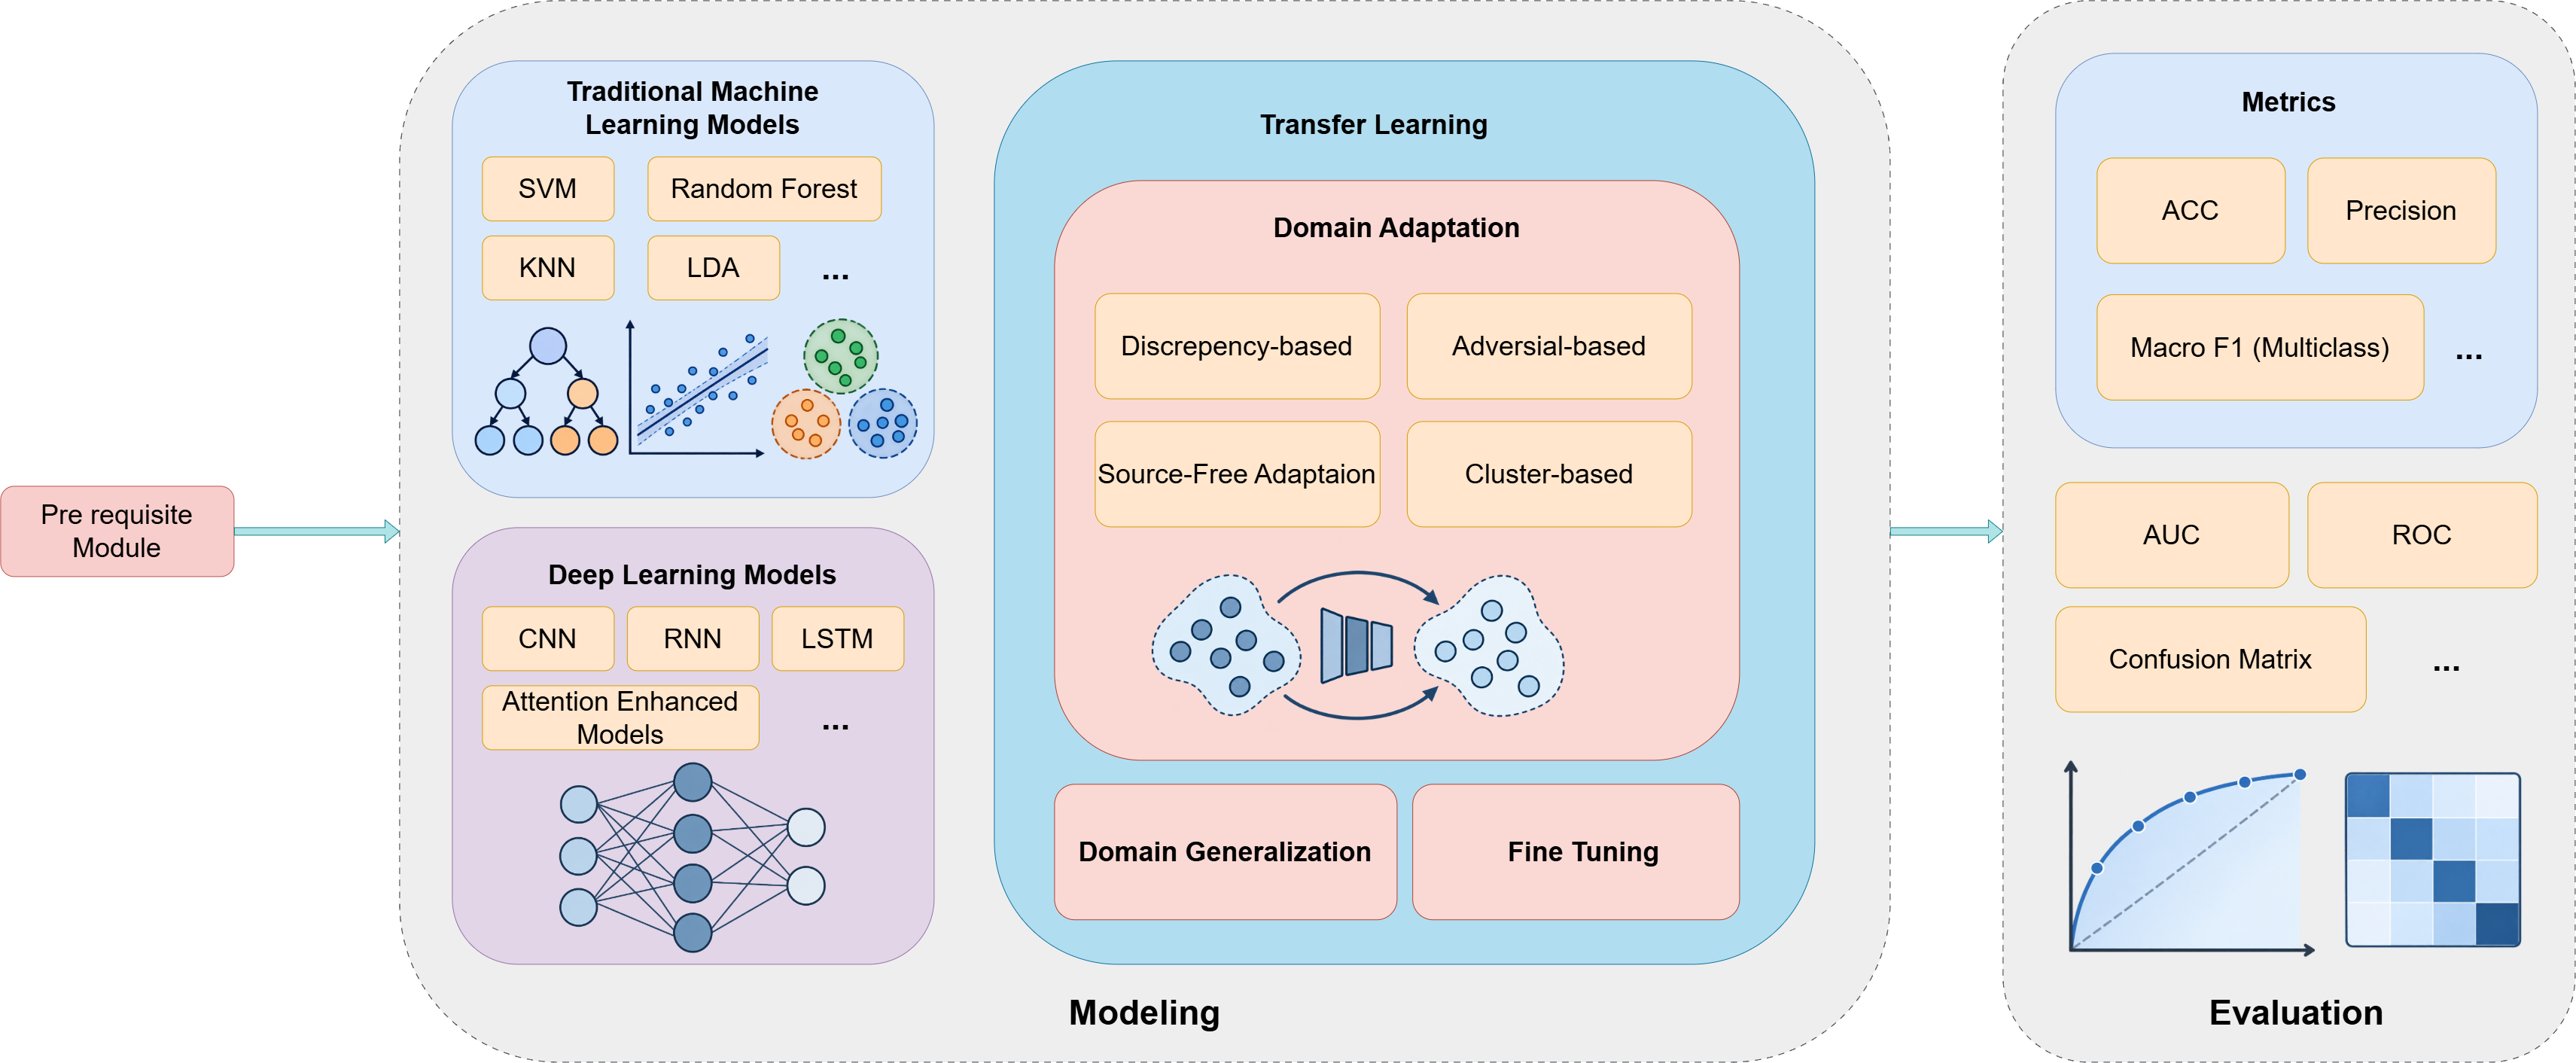
\includegraphics[width=\linewidth]{pictures/methodologies.png}

    \caption{Overview of modeling and evaluation approaches in EEG based emotion recognition, illustrating traditional machine learning, deep learning, transfer learning strategies, and commonly employed performance evaluation measures.}

    \label{fig:eeg_modeling_evaluation}
\end{figure*}


The modeling stage of EEG based emotion recognition encompasses a diverse range of computational approaches designed to extract discriminative representations and classify emotional states from neural activity. As illustrated in Fig.~\ref{fig:eeg_modeling_evaluation}, these approaches broadly include traditional machine learning models, deep learning architectures, and transfer learning strategies. Conventional methods, such as support vector machines, random forests, k-nearest neighbors, and linear discriminant analysis, generally rely on predefined EEG features, whereas deep learning architectures, including convolutional neural networks, recurrent neural networks, LSTMs, and attention based models, enable increasingly complex representations of temporal, spectral, and spatial information. To address variations across subjects, recording sessions, and datasets, transfer learning approaches incorporate domain adaptation, domain generalization, and fine tuning strategies. Domain adaptation can further involve discrepancy minimization, adversarial alignment, clustering based methods, or source free adaptation when original source data are unavailable \cite{li2024cadddccnn}. As shown in Fig.~\ref{fig:eeg_modeling_evaluation}, the resulting models are evaluated using complementary measures, including classification accuracy, precision, macro averaged F1 score, receiver operating characteristic (ROC) analysis, area under the ROC curve (AUC), and confusion matrices. Considering these measures together provides a more comprehensive assessment of classification performance and class specific errors. Consequently, selecting an appropriate modeling approach requires balancing predictive performance, computational complexity, generalizability, and evaluation reliability.


Overall, CNN centric models are often best when local spatial and spectral patterns dominate and training data are moderate, whereas RNN/sequential models are preferable when temporal dynamics carry most discriminative information but can be harder to optimize. Topology aware encoders are most useful when cross electrode coupling is central to the affective mechanism, although they can be sensitive to montage and preprocessing \cite{zhong2020rgnn}. Attention/transformer style models are best when long range, context dependent interactions are critical, but they demand careful regularization and protocol rigor to prevent leakage and spurious saliency. Across all families, the strongest empirical lesson is that domain generalizable deep EEG emotion recognition depends as much on disciplined evaluation and artifact aware preprocessing as on architecture choice \cite{cqlaih2018artifact}.

\paragraph{Standalone Models}
\label{sec:standalone_models}

Standalone deep models learn a single end to end mapping from EEG inputs to emotion labels and are therefore a useful lens for domain generalization: they expose how much cross subject/cross session robustness can be obtained from architectural inductive bias and disciplined training alone, without additional fusion, multi branch alignment, or auxiliary objectives. In EEG emotion recognition, standalone baselines are valuable because they isolate representation learning in $\phi_{\theta}(\mathbf{X})$ and reduce confounding factors like, heterogeneous feature fusion and branch specific preprocessing, making results easier to reproduce and compare across protocols \cite{saydn2020deeplear}. Their model specification typically centers on backbone type (CNN/RNN), input encoding like raw, time and frequency, or spatial maps, and depth and width trade offs that control expressivity versus overfitting and subject memorization \cite{li2022efficientcnncl}.

Independent deep learning architectures were extensively studied in emotion recognition via EEG due to their ability to learn useful data representations without having to rely solely on hand-crafted features. Convolutional neural networks (CNNs) were used by Cheng et al. to extract spatial-spectral characteristics of EEG signals. Although convolutional layers have proved effective at capturing local dependencies, their relatively small receptive field might not allow capturing long-term temporal dependencies without the use of any temporal mechanisms.

Apart from the architectural aspects, issues involving evaluation and efficiency must also be considered. For instance, the study by Egger et al.~\cite{megger2019emotionr} demonstrated that deep learning approaches should be evaluated against feature-engineered classifiers under controlled experiments in order to determine recognition performance. Yet, unbalanced distribution of datasets may result in an overly optimistic evaluation due to correlation of EEG samples both in the training and test sets. At the same time, the paper by Suhaimi et al.~\cite{nssuha2020eegbased} deals with the problem of differences in methodologies applied for the evaluation of performance of methods that are used to classify emotions on the basis of EEG signals and demonstrates how different procedures of preprocessing affect the result. With regard to computational efficiency, there has been research on lightweight methodologies of EEG signal classification conducted by Wank et al.~\cite{sbwank2019ikknpred}. While providing certain advantages in terms of memory and speed of inference, such methods might lack capacity to recognize patterns of EEG data.

A generic standalone convolutional block can be summarized as
\begin{equation}
\mathbf{H}^{(l)}=\sigma\!\left(\mathbf{W}^{(l)} * \mathbf{H}^{(l-1)}+\mathbf{b}^{(l)}\right),
\end{equation}
where $\mathbf{H}^{(l-1)}$ and $\mathbf{H}^{(l)}$ are the input/output feature maps at layer $l$, $\mathbf{W}^{(l)}$ and $\mathbf{b}^{(l)}$ are trainable weights and biases, $*$ denotes convolution over the chosen EEG tensorization like, channel$\times$time or time and frequency maps, and $\sigma(\cdot)$ is a nonlinearity. CNN only standalone models are attractive because they match spatial locality in EEG topographies and time and frequency representations, and they avoid multi branch fusion instabilities, which can otherwise obscure whether gains come from architecture or from fusion heuristics.

Overall, standalone models are best when the goal is clean benchmarking and ablation driven insight: they provide the most interpretable evidence of what inductive bias (CNN vs.\ RNN) and what training protocol contribute to performance. CNN only standalones are typically preferred when computations must be efficient and when discriminative cues are localized in time and frequency or spatial maps, while RNN family standalones are preferred when long range temporal dynamics are central but can be slower and harder to optimize. For real time affective systems with strict latency/memory constraints, lightweight standalone designs remain the practical choice, though they require careful regularization and input encoding to avoid underfitting.

\paragraph{Attention Enhanced Models}
\label{sec:attention_enhanced_models}

Attention enhanced models extend deep EEG emotion recognition by making relevance a learnable function of the input, rather than a fixed property of particular channels or time points. This design choice is closely tied to domain generalization: because emotion relevant EEG evidence can appear sparsely in time and vary in spatial distribution across subjects, attention provides a content adaptive mechanism to emphasize discriminative substructures while suppressing nuisance variability. Consequently, attention based model descriptions emphasize (i) the granularity of attention (channel wise, temporal, or joint), (ii) the scoring function that produces weights, and (iii) the integration rule that mixes attended features with a backbone representation, since these choices determine whether the model learns robust affective cues instead of memorizing subject specific patterns \cite{tao2020channelselfatt}.


Beyond the attention applied to each channel, Zhang et al. studied the spatial and temporal relations between EEG signals in order to obtain informative neural interactions during emotion processing. However, despite the benefits that can be achieved by modeling the distributed brain activity, there are still issues of artifacts, referencing approaches, and segmentation in connectivity representations and temporal weighting. On a more general note, Roy et al.~\cite{yroyhb2019deeplear} gave an overview of the use of deep learning approaches in the analysis of EEG signals, which offers useful information about the design and evaluation of deep architectures. This is particularly relevant for attention-based models where improper data splitting and control can cause overoptimistic results.

Transformer style attention increasingly appears because emotion relevant cues exhibit long range interactions across time and channels. Self attention defines queries, keys, and values as $\mathbf{Q}=\mathbf{H}\mathbf{W}_Q$, $\mathbf{K}=\mathbf{H}\mathbf{W}_K$, and $\mathbf{V}=\mathbf{H}\mathbf{W}_V$, and it computes \begin{equation} \mathrm{Attn}(\mathbf{Q},\mathbf{K},\mathbf{V})=\mathrm{softmax}\!\left(\frac{\mathbf{Q}\mathbf{K}^\top}{\sqrt{d}}\right)\mathbf{V}, \end{equation} which yields data adaptive aggregation over tokens that represent channels, time steps, or time frequency patches. Attention mechanisms fit EEG decoding because relevance concentrates in subsets of electrodes and epochs, so learned weighting acts as a soft selection operator that complements convolution or recurrence. Attention based designs also support post hoc analysis via saliency like maps, yet interpretability remains conditional because weight patterns do not necessarily imply causal importance \cite{tao2020channelselfatt}.

Attention enhanced models introduce adaptive reweighting across channels and time, so they prioritize salient electrodes and temporal segments while suppressing irrelevant activity. Channel wise attention often learns a gating vector $\boldsymbol{\alpha}\in[0,1]^C$ and produces a reweighted signal $\tilde{\mathbf{X}}=\mathrm{diag}(\boldsymbol{\alpha})\mathbf{X}$, where \begin{equation} \boldsymbol{\alpha}=\sigma\!\left(\mathbf{W}_2\,\delta(\mathbf{W}_1\,\mathrm{pool}(\mathbf{X}))\right), \end{equation} and $\mathrm{pool}(\cdot)$ aggregates across time. Channel attention also acts as an implicit sensor selection mechanism, which reduces sensitivity to noisy electrodes and facilitates reduced montage systems \cite{jxingk2018adaptive}. Temporal attention highlights salient segments within a trial, which matters when affect evolves gradually rather than instantaneously. Attention enhanced models also introduce optimization sensitivity, so they require careful learning rate schedules and regularization to avoid unstable convergence.

Overall, attention enhanced models are best when discriminative evidence is sparse or subject varying in space/time and when robustness benefits from emphasizing salient substructures. Channel attention mechanisms are most useful when sensor noise or electrode relevance varies, enabling soft channel selection, whereas temporal attention is most useful when emotions evolve over time and informative segments are localized. However, attention modules increase optimization sensitivity and can overfit in small data settings, so they are most reliable under careful regularization, disciplined evaluation splits, and protocol checks that reduce leakage and annotation bias.


\paragraph{Hybrid Models}
\label{sec:hybrid_models}

Hybrid deep models for EEG emotion recognition combine multiple operator families like, convolution, recurrence, attention, graph/relational modules to capture complementary structure across space, time, and frequency. From a domain generalization perspective, hybridization is motivated by the fact that emotion relevant EEG cues can shift in their dominant form across subjects and sessions as, some subjects exhibit discriminative spatial patterns, others exhibit stronger temporal dynamics. Thus, hybrid models assume that no single inductive bias is universally sufficient and instead aim to learn representations that remain robust under nuisance variability by integrating multiple views of the signal. The model specification therefore emphasizes the participating modules, the fusion stage, and coordination constraints (normalization, scale matching, and regularization) needed to stabilize training and prevent a single branch from dominating \cite{li2022mvsstma}.

Apart from representation learning, architecture complexity and evaluation consistency also matter. In their review on EEG emotion recognition methods, Suhaimi et al.~\cite{nssuha2020eegbased} pointed out the variations in preprocessing, experimental setup, and evaluation procedure that hinder comparison between studies. The works by Egger et al. on alternative modeling methods serve as the starting point for evaluating the trade-off between model complexity and emotion recognition performance. The interaction between different modules in the hybrid architecture could cause optimization issues, which makes controlled ablation studies necessary for estimating the contribution of each module. Li et al.~\cite{wlizzh2021physiolo} introduced some ways of learning complementary representations from physiological signals, showing the possibility of using different feature learning mechanisms. However, the coordination of several processing modules increases the complexity of implementation and sensitivity to training settings. Overall, it seems that the effectiveness of hybrid EEG emotion recognition models should be proved by systematic ablation studies, consistent preprocessing, and proper cross-subject evaluation.

CNN and RNN hybrids commonly pass convolutional embeddings $\mathbf{h}_t$ (local spatial/spectral features) into a gated recurrent unit (GRU) to model longer temporal dependencies. A GRU update is:
\begin{equation}
\mathbf{z}_t=\sigma(\mathbf{W}_z\mathbf{h}_t+\mathbf{U}_z\mathbf{s}_{t-1}),\quad
\mathbf{r}_t=\sigma(\mathbf{W}_r\mathbf{h}_t+\mathbf{U}_r\mathbf{s}_{t-1}),
\end{equation}
\begin{equation}
\tilde{\mathbf{s}}_t=\tanh(\mathbf{W}\mathbf{h}_t+\mathbf{U}(\mathbf{r}_t\odot \mathbf{s}_{t-1})),\quad
\mathbf{s}_t=(1-\mathbf{z}_t)\odot \mathbf{s}_{t-1}+\mathbf{z}_t\odot \tilde{\mathbf{s}}_t,
\end{equation}
where $\mathbf{s}_t$ is the hidden state, $\mathbf{z}_t$ and $\mathbf{r}_t$ are update/reset gates, and $\odot$ denotes element wise multiplication. This structure encodes multi scale context by pairing local feature extraction (CNN) with sequential memory (RNN/GRU), which is useful when affective dynamics evolve over extended time.

Overall, hybrid models are best when emotion cues are multi factorial such as simultaneously spatial, temporal, and relational and when the dataset/protocol provides enough coverage to train multi module systems without overfitting. CNN and RNN (or CNN and Transformer) hybrids are often preferable when both short term rhythmic patterns and longer temporal context are discriminative, whereas topology aware+temporal hybrids are preferable when inter channel coupling is central to affect representation. However, because hybrids introduce optimization sensitivity and branch dominance risks, they are most reliable under careful normalization, regularization, and disciplined ablations that separate true architectural benefit from preprocessing or split artifacts.

\section{Datasets and Comparative Study}

A dataset-centric comparative evaluation is essential for assessing EEG-based emotion recognition methods because reported performance is strongly influenced by recording protocols, emotional stimuli, electrode configurations, annotation strategies, preprocessing procedures, and training--testing partitions. Consequently, meaningful comparisons require consistent documentation of dataset characteristics and evaluation protocols, particularly when distinguishing subject-dependent from subject-independent performance. The new surveys reveal the fact that variations in signal processing, segmentation, normalization, and data splitting can greatly affect reproducibility and the assessment of improvements in model performance \cite{li2022tutorial}.


\begin{table*}[tp]
\centering
\small
\setlength{\tabcolsep}{2pt}
\renewcommand{\arraystretch}{1.07}

\caption{Comparative overview of widely used EEG-based emotion recognition datasets.}

\label{tab:dataset_attr}

\begin{tabular}{@{}
>{\raggedright\arraybackslash}p{0.115\textwidth}
>{\centering\arraybackslash}p{0.047\textwidth}
>{\centering\arraybackslash}p{0.050\textwidth}
>{\centering\arraybackslash}p{0.049\textwidth}
>{\centering\arraybackslash}p{0.079\textwidth}
>{\raggedright\arraybackslash}p{0.100\textwidth}
>{\raggedright\arraybackslash}p{0.120\textwidth}
>{\raggedright\arraybackslash}p{0.090\textwidth}
>{\raggedright\arraybackslash}p{0.136\textwidth}
>{\raggedright\arraybackslash}p{0.124\textwidth}
@{}}

\toprule

\textbf{Dataset} &
\textbf{Subje\newline cts} &
\textbf{Sessi\newline ons} &
\textbf{EEG Channels} &
\textbf{Sampling rate} &
\textbf{Stimuli} &
\textbf{Label Space} &
\textbf{Ratings} &
\textbf{Modalities} &
\textbf{Notes} \\

\midrule

DEAP \cite{koelstra2012deap} &
32 &
1 &
32 &
512 Hz &
40 music videos (60 s) &
Dimensional &
V/A/D + liking (1--9) &
EEG + peripheral + video &
Strong baseline; clear trial structure \\

\lightrowsep

SEED \cite{seed_page,zheng2015seed} &
15 &
3 &
62 &
200 Hz &
15 film clips ($\sim$4 min) &
3 class &
Self report &
EEG + eye tracking &
Multi session; DE features available \\

\lightrowsep

SEED-IV \cite{seediv_page,zheng2019emotionmeter} &
15 &
3 &
62 &
200 Hz &
72 clips (24/session) &
4 class &
PANAS style &
EEG + eye tracking &
Fixed 4 s segments \\

\lightrowsep

DREAMER \cite{katsigiannis2018dreamer} &
23 &
1 &
14 &
128 Hz &
18 clips (65--393 s) &
Dimensional &
V/A/D (1--5) &
EEG + ECG &
Wearable oriented, low channels \\

\lightrowsep

MAHNOB HCI \cite{soleymani2012mahnob,kukhilava2025evaluation} &
27 &
1 &
32 &
256 Hz &
20 videos &
Dimensional + tags &
V/A/D + keywords &
EEG + multimodal &
Rich synchronized modalities \\

\lightrowsep

AMIGOS \cite{amigos2018} &
40 &
2 &
14 &
128 Hz &
16 short + 4 long videos &
Dimensional + basic &
V/A/D (1--9) &
EEG + multimodal &
Includes group/social context \\

\lightrowsep

ASCERTAIN \cite{subramanian2018ascertain} &
58 &
1 &
1 &
32 Hz &
36 clips (51--127 s) &
Dimensional + personality &
V/A + Big Five &
EEG + multimodal &
Single dry sensor, low bandwidth \\

\lightrowsep

MPED \cite{song2019mped} &
23 &
1 &
62 &
-- &
28 videos &
7 class &
Ratings + labels &
EEG + multimodal &
Fine grained discrete emotions \\

\lightrowsep

FACED \cite{chen2023faced} &
123 &
1 &
32 &
250/1000 Hz &
28 videos ($\sim$66 s) &
9-class &
0--7 ratings + V/A &
EEG &
Large scale dataset \\

\lightrowsep

GAMEEMO \cite{alakus2021gameemo} &
28 &
1 &
14 &
128 Hz &
4 games (5 min) &
4 class &
Protocol based &
EEG &
Game induced emotions \\

\bottomrule

\end{tabular}

\end{table*}

There exist two types of annotation paradigms that are usually used in EEG emotion recognition datasets: dimensional representations (valence, arousal, and dominance), and discrete representations (emotions classified into predefined classes). The dimensional representation paradigm is based on the established affective models, such as the circumplex model. At the same time, self-assessment tools like the Self-Assessment Manikin (SAM) help to annotate subjective emotions. As shown in Table~\ref{tab:dataset_attr}, different common datasets have a wide variety of attributes: number of participants, number of EEG channels, sampling rate, emotional stimuli, type of annotation, and modality types. DEAP, DREAMER, MAHNOB-HCI, AMIGOS, and ASCERTAIN are mainly used for dimensional affect recognition, and SEED, SEED-IV, MPED, FACED, and GAMEEMO are used for discrete emotional recognition with various classification complexity.

To justify dataset choice in an abstract in method agnostic sense, we recommend evaluating datasets along five axes:
\textit{(1) physiological fidelity} (channel density and sampling rate),
\textit{(2) label validity} (self report driven vs.\ clip assigned; discrete vs.\ continuous),
\textit{(3) generalization support} (subject count; multi session availability),
\textit{(4) ecological validity} (naturalistic stimuli, social interaction, task based affect),
and \textit{(5) reproducibility support} (documentation, file structure, provided features).
These criteria align with the main reproducibility concerns highlighted in recent EEG emotion recognition methodological reviews. \cite{brookshire2024leakage}

\begin{table*}[tp]
\centering
\normalsize

\setlength{\tabcolsep}{2pt}
\renewcommand{\arraystretch}{1.07}

\caption{Scenario-driven selection of EEG emotion recognition datasets for evaluating cross-subject generalization, cross-session robustness, wearable deployment, multimodal fusion, dimensional affect prediction, and discrete emotion classification.}

\label{tab:scenario_map}

\begin{tabularx}{\textwidth}{@{}
>{\raggedright\arraybackslash}p{0.205\textwidth}
>{\raggedright\arraybackslash}p{0.265\textwidth}
>{\raggedright\arraybackslash}X
@{}}

\toprule

\textbf{Scenario / goal} &
\textbf{Recommended datasets} &
\textbf{Rationale} \\

\midrule

Cross subject (unseen user) modeling
&
FACED \cite{chen2023faced};
SEED \cite{zheng2015seed};
SEED IV \cite{zheng2019emotionmeter}
&
FACED contains a substantially larger participant cohort than many
commonly used EEG emotion datasets, making it particularly useful for
estimating inter subject variability and evaluating subject independent
models. SEED and SEED-IV are also widely used in cross subject evaluation
and provide structured experimental protocols suitable for separating
training and testing subjects \cite{apicella2024neucom_systematic}.
\\

\lightrowsep

Cross session robustness (same users, different days)
&
SEED \cite{zheng2019stablepatterns};
SEED-IV \cite{chen2021frontiers_msmda}
&
SEED contains repeated recordings from the same participants across
three sessions separated in time, while SEED-IV follows a comparable
multi session design. These properties permit explicit evaluation
of session drift and cross session generalization rather than
relying only on single session performance
\cite{apicella2024neucom_systematic}.
\\

\lightrowsep

Wearable / low channel deployment constraints
&
DREAMER \cite{katsigiannis2018dreamer};
AMIGOS \cite{amigos2018};
GAMEEMO \cite{alakus2021gameemo};
ASCERTAIN \cite{geng2025dlreview}
&
DREAMER and AMIGOS use wearable, relatively low channel EEG systems,
while GAMEEMO has been investigated under single channel EEG
configurations. ASCERTAIN was specifically constructed using commercial
sensing equipment. These datasets are therefore useful when evaluating
reduced channel, consumer oriented, or practically deployable EEG
configurations \cite{dadebayev2022commercial}.
\\

\lightrowsep

Multimodal fusion / sensor complementarity
&
DEAP \cite{koelstra2012deap};
MAHNOB HCI \cite{soleymani2012mahnob};
AMIGOS;
MPED \cite{song2019mped};
ASCERTAIN \cite{subramanian2018ascertain}
&
These datasets provide EEG together with one or more synchronized
complementary modalities, including ECG, GSR, respiration, eye related
information, facial video, or other peripheral physiological signals.
They therefore enable feature level, decision level, and hybrid
multimodal fusion as well as modality ablation experiments
\cite{wang2024csur_researchprogress}.
\\

\lightrowsep

Dimensional affect (valence/arousal) as primary target
&
DEAP \cite{koelstra2012deap};
DREAMER;
MAHNOB-HCI \cite{soleymani2012mahnob};
AMIGOS;
ASCERTAIN
&
These datasets provide affective annotations based primarily on
valence and arousal, with several also reporting dimensions such
as dominance. Consequently, they are appropriate for continuous
affect prediction as well as binary or quadrant based classification
after explicitly defined discretization thresholds
.
\\

\lightrowsep

Discrete multi class emotion classification
&
SEED-IV \cite{PeerJCS2065};
MPED;
FACED;
GAMEEMO
&
SEED-IV provides four discrete affective classes, MPED contains seven
discrete emotion categories, and FACED provides a finer grained
nine category affective taxonomy. GAMEEMO provides four game induced
affective conditions. These datasets are therefore suitable for
multi class evaluation, including class wise recall, F1 score,
confusion matrix analysis, and investigation of class specific
errors \cite{PeerJCS2065}.
\\

\bottomrule

\end{tabularx}

\end{table*}

Table~\ref{tab:scenario_map} further indicates the compatibility of different datasets for particular experimental goals. In addition to providing many more participants for the research of cross-subject generalization studies, FACED offers an increased number of participants relative to other datasets. Different recording sessions within SEED and SEED-IV enable inter-session variability analysis \cite{seed_page,seediv_page}. The datasets which can be used for wearable devices applications and other purposes include low-channel EEG datasets of DREAMER and AMIGOS. ASCERTAIN is yet another dataset which may be used in the research on low-channel physiological sensing and users' emotions. Finally, multimodal datasets, such as DEAP and MAHNOB-HCI, allow for the analysis of complementary physiological and behavioral information using feature fusion methods.

Overall, there is no benchmark that covers all possible EEG emotion recognition scenarios. Thus, the choice of a dataset should be based on the particular recognition scenario, emotion label structure, acquisition process, modalities used, and evaluation protocol rather than accuracy reported by the authors. In particular, research on generalization should focus on subject-disjoint evaluation, proper preprocessing, clear data splitting, and cross-session or cross-dataset validation if applicable.


\subsection{Performance Metrics}
\label{subsec:performance_metrics}

Performance metrics provide a quantitative basis for evaluating EEG-based emotion recognition models, enabling comparisons of classification accuracy, class-specific errors, discrimination, and generalization. Their selection is particularly important because EEG datasets differ in emotional categories, class distributions, and experimental protocols. Therefore, depending on one measure might overlook some weaknesses, particularly in case of class imbalance and/or subject-independent evaluation. In recent researches, it has been stressed that different parameters and frameworks should be used for comparison \cite{kukhilava2025evaluation}.

Accuracy, precision, and recall are three basic evaluation criteria for classification problems, all obtained from the confusion matrix. The accuracy metric represents the percentage of correctly classified samples, while the precision criterion represents the quality of positive prediction, and the recall metric represents the percentage of correctly identified positive samples. While the accuracy metric gives an intuitive idea about the algorithm’s performance, it can be deceptive in cases of unbalanced emotional classes. In binary classification problem, the number of true positives, true negatives, false positives, and false negatives is denoted as $TP$, $TN$, $FP$, $FN$, respectively, where $N=TP+TN+FP+FN$. The definition of these metrics is

\begin{equation}
\begin{aligned}
\mathrm{Accuracy} &= \frac{TP+TN}{N},\\[3pt]
\mathrm{Precision} &= \frac{TP}{TP+FP},\\[3pt]
\mathrm{Recall} &= \frac{TP}{TP+FN}.
\end{aligned}
\label{eq:basic_metrics}
\end{equation}

The F1 score measures the balance between precision and recall through the harmonic mean of the two. It is especially useful in an unbalanced emotion recognition task since it takes into account both false negatives and false positives, though it does not consider the true negatives.

\begin{equation}
\mathrm{F1} =
\frac{2\,\mathrm{Precision}\cdot\mathrm{Recall}}
{\mathrm{Precision}+\mathrm{Recall}}.
\label{eq:f1}
\end{equation}

The macro F1 equally weights all emotions through averaging the value of F1 for each individual emotion:

\begin{equation}
\mathrm{MacroF1} =
\frac{1}{C}\sum_{c=1}^{C}\mathrm{F1}_c,
\label{eq:macro_f1}
\end{equation}

where C is the number of emotion classes. Unlike accuracy, the macro F1 score does not depend on class occurrence and is therefore useful in assessing multiclass datasets where there is an imbalance in the distribution of the data set.

The balanced accuracy is yet another measure that accounts for class imbalance by assigning equal importance to sensitivity. The balanced accuracy in the binary classification model is given by:

\begin{equation}
\begin{aligned}
\mathrm{BalAcc}
&= \frac{1}{2}(\mathrm{TPR}+\mathrm{TNR})\\[3pt]
&= \frac{1}{2}
\left(
\frac{TP}{TP+FN}
+
\frac{TN}{TN+FP}
\right).
\end{aligned}
\label{eq:balacc}
\end{equation}

Balanced accuracy is commonly applied when there are more than two classes, and it is computed as the mean recall across all classes, $\mathrm{BalAcc}=\frac{1}{C}\sum_{c=1}^{C}\mathrm{Recall}_c$. Unlike F1-macro which takes into account both precision and recall, balanced accuracy emphasizes only the sensitivity of emotions.

The area under the receiver operating characteristic curve (ROC-AUC) allows us to assess the discrimination power of the classifier. Unlike accuracy and F1 score, which depend on a selected operating threshold, AUC measures how effectively prediction scores distinguish positive and negative instances.

\begin{equation}
\mathrm{AUC} =
\int_{0}^{1}
\mathrm{TPR}(\mathrm{FPR})\,d\mathrm{FPR},
\label{eq:auc}
\end{equation}

where $\mathrm{FPR}=FP/(FP+TN)$ and $\mathrm{TPR}=TP/(TP+FN)$. Although AUC provides a threshold-independent discrimination measure, it does not assess probability calibration or classification performance at a particular threshold. Multiclass evaluations should therefore specify the averaging and one-versus-rest or one-versus-one strategy employed.

Besides classification performance measures, consistency among participants and repetitions in experiments is crucial to evaluate generalization ability. Cross-validation and leave-one-subject-out (LOSO) evaluation help quantify performance variability, particularly when EEG distributions differ among individuals. For $K$ evaluation folds, with metric value $m_k$ for fold $k$, the mean and sample standard deviation are calculated as

\begin{equation}
\overline{m} =
\frac{1}{K}\sum_{k=1}^{K}m_k,
\qquad
s =
\sqrt{
\frac{1}{K-1}
\sum_{k=1}^{K}
(m_k-\overline{m})^2
}.
\label{eq:mean_std}
\end{equation}

Reporting $\overline{m}\pm s$ provides information about both average performance and variability, although standard deviation should not be interpreted as a confidence interval. Subject-level analysis and consistent partitioning of data is crucial in determining unstable performance and preventing data leakage \cite{brookshire2024leakage}.

Moreover, statistical tests need to determine whether the improvements shown are consistent between the corresponding evaluation units. In cases where the paired differences are normally distributed, a paired $t$ test could be used. Alternatively, in the case of symmetrically distributed paired differences, the Wilcoxon signed-rank test can be considered. Effect size measures, confidence intervals, and correction for multiple comparisons must accompany the significance tests in order to demonstrate the significance of the differences between the performances.

In conclusion, there is a need for more complementary evaluation measures instead of accuracy measures alone in order to conduct reliable evaluation of EEG emotion recognition models. Macro F1 and balanced accuracy are particularly valuable for imbalanced classification problems, whereas ROC-AUC is used to assess discrimination ability without thresholds.


\subsection{Experimental Analysis}
\label{subsec:experimental_analysis}

Experimental evaluation of emotion recognition systems using EEG needs to be understood in light of the evaluation strategy since the extent of subject overlap between the training and testing data has a direct impact on the level of task difficulty \cite{nath2020lstm}. In subject dependent evaluation, participant specific knowledge can be learned through training, while in subject independent evaluation, the validity of emotion representations for novel participants is examined. Transfer learning evaluation goes one step further by testing whether knowledge gained from a source can be transferred to a target domain \cite{li2022compbiomed_metatransfer_connectivity}.Consequently, accuracy values obtained under these settings should not be compared without considering the dataset, feature representation, number of emotion classes, and train test protocol \cite{cimtay2020sensors_pretrainedcnn}.

This distinction is especially important for EEG because inter subject variability, session to session non stationarity, electrode configuration, and stimulus design can substantially alter the underlying feature distribution \cite{chen2021meernet}. Earlier comparisons already showed a considerable difference between intra subject and inter subject recognition, while recent deep architectures increasingly address this problem through spatial and spectral modeling, graph learning, attention, domain adaptation, and transfer learning. The following comparisons therefore retain the original experimental conditions and reported accuracies rather than combining heterogeneous results into a single aggregate score.

\subsubsection{Subject Dependent Evaluation}
\label{subsubsec:subject_dependent_evaluation}

Subject dependent evaluation uses EEG from the same participant population in both model development and testing, typically through within subject partitioning or cross validation. This setting is useful for measuring the representational capacity of a model when subject specific calibration is available, and it generally produces higher accuracies than subject independent evaluation. The progression in
Subject dependent EEG emotion recognition has been extensively investigated using conventional feature representations and increasingly sophisticated deep learning architectures. The comparative overview of representative works is given in Table~\ref{tab:subject_dependent_results}. In earlier works, EEG features were mostly handcrafted, such as differential entropy (DE), power spectral density (PSD), and spatial EEG features, used together with convolutional or graph neural network models \cite{xiong2025cnnkanf2ca}. The most recent studies use adaptive graph convolution, attention, Transformers, and multi branch feature fusion to account for complicated spatial, spectral, and temporal dependencies involved in emotional response processing \cite{ding2025dgat}. This indicates that there is an inclination to learn complementary representations of EEG data from neurons rather than focusing on specific frequency bands or electrodes.

From Table~\ref{tab:subject_dependent_results}, it is observed that many studies have attained high accuracies for subject dependent evaluation on popular databases such as DEAP, SEED, SEED-IV, and DREAMER. Nonetheless, the reported results show significant heterogeneity of methodologies applied, including various configurations of emotion labels, input features, electrode placement, data segmentation, and validation strategy. Specifically, while some studies perform evaluation on individual EEG windows, others use trial wise grouping or other cross validation schemes. This is an essential issue since similar EEG segments presented in both training and testing datasets can provide overestimated accuracy. In addition, the difference between binary valence arousal classification, three class emotion recognition, and emotion categories make direct comparison of reported accuracies difficult. Therefore, the results presented in Table~\ref{tab:subject_dependent_results} should be treated as specific to the experiment conducted and cannot be viewed as ranking of classification architectures. Nonetheless, the results show the ability of deep learning to detect emotion related EEG patterns in individuals.

\begin{sidewaystable*}[p]
\centering
\caption{Comparative overview of representative subject-dependent EEG-based emotion recognition studies. Results are reported under their original experimental conditions. Differences in experimental protocols limit direct comparability across datasets}
\label{tab:subject_dependent_results}

\scriptsize
\setlength{\tabcolsep}{3.0pt}
\renewcommand{\arraystretch}{1.18}

\begin{tabularx}{\textheight}{
>{\raggedright\arraybackslash}p{3.15cm}
>{\raggedright\arraybackslash}X
>{\raggedright\arraybackslash}X
>{\raggedright\arraybackslash}p{3.65cm}
>{\raggedright\arraybackslash}p{5.15cm}}

\toprule
\textbf{Study} &
\textbf{Input feature(s)} &
\textbf{Method} &
\textbf{Dataset / evaluation} &
\textbf{Accuracy (\%)} \\
\midrule

Song et al. \cite{song2020dgcnn} &
DE, PSD, DASM, RASM, and DCAU EEG descriptors represented over electrode graphs &
DGCNN with dynamically learned inter electrode adjacency relationships &
SEED; subject dependent &
$90.40 \pm 8.49$ \\

\lightrowsep

Deng et al. \cite{deng2021sfenet} &
Multichannel EEG reorganized into symmetry aware spatial representations preserving electrode topology &
SFE-Net with symmetrical spatial feature extraction and convolutional representation learning &
SEED; subject dependent &
99.19 \\

\lightrowsep

Jia et al. \cite{jia2020sstemotionnet} &
Three dimensional differential entropy representations encoding spatial, spectral, and temporal information &
SST-EmotionNet using spatial, spectral and temporal attention with a 3D dense architecture &
SEED and SEED-IV; subject dependent &
SEED: $96.02 \pm 2.17$;
SEED-IV: $84.92 \pm 6.66$ \\

\lightrowsep

Guo et al. \cite{guo2022dcot} &
Differential entropy features extracted from the principal EEG frequency bands &
DCoT combining depthwise convolutional representation learning with a Transformer encoder &
SEED; subject dependent &
93.83 \\

\lightrowsep

Ding et al. \cite{ding2025dgat} &
DE features extracted by STFT from four frequency bands for DEAP and five bands for SEED;
EEG electrodes form graph nodes &
DGAT with a dynamically updated adjacency matrix and multi head graph attention
for adaptive inter channel relationship learning &
DEAP and SEED; five fold subject dependent cross validation &
SEED: $94.00 \pm 2.60$;
DEAP-V: $93.55 \pm 3.89$;
DEAP-A: $93.19 \pm 3.65$ \\

\lightrowsep

Xiong et al. \cite{xiong2025cnnkanf2ca} &
DE, PSD, EVI, and ASI features from four frontal channels
(FP1, FP2, AF3, AF4), mapped into pseudo RGB feature matrices &
CNN-KAN-F2CA integrating convolutional feature extraction,
FFT based frequency channel attention, and a Kolmogorov and Arnold Network classifier &
SEED and DEAP; single subject subject dependent evaluation &
SEED three class: 97.45;
DEAP-V: 90.03;
DEAP-A: 91.33;
DEAP VA four class: 89.16 \\

\lightrowsep

Lin et al. \cite{lin2026pconvcapsnet} &
Bandpass filtered and baseline corrected multichannel EEG transformed
into time and frequency representations &
PconvCapsNet using selective partial convolution with synchronized channel bypass
and primary and dense capsules with dynamic routing &
DEAP and DREAMER; subject dependent &
DEAP: A 98.03, V 97.81, D 98.11;
DREAMER: A 97.20, V 96.49, D 97.04 \\

\lightrowsep

Soundariya and Thangaraj \cite{soundariya2026awtnet} &
Multiscale EEG components obtained through hierarchical wavelet packet decomposition
and EWT with Kalman filtering &
AWT-Net combining multiscale wavelet analysis, multi-head self-attention,
a hybrid spatio temporal Transformer, and adaptive focal loss &
DEAP; five fold subject dependent evaluation &
99.61 window level;
99.30 trial wise grouped \\

\lightrowsep

Hua et al. \cite{hua2026bradnet} &
Continuous temporal EEG for the spatio temporal branch and spectral spatial
time and frequency maps preserving electrode topology for the second branch &
BRAD-Net with brain region constrained self attention,
CNN and Transformer temporal modeling,
multi scale residual spectral spatial learning, and feature fusion &
DEAP and DREAMER; subject dependent 10 fold cross validation &
DEAP: V $97.44 \pm 1.19$, A $97.70 \pm 1.13$, D $97.97 \pm 1.14$;
DREAMER: V $99.66 \pm 0.22$, A $99.78 \pm 0.14$, D $99.80 \pm 0.16$ \\

\lightrowsep

Liu et al. \cite{liu2026taformer} &
Four dimensional dense EEG representation preserving channel topology
together with temporal and multidimensional feature structure &
TaFormer using triplet attention to learn cross dimensional,
global spatial, and long range temporal information,
followed by dual channel dynamic feature fusion &
DEAP, SEED, DREAMER, and HBUED; subject dependent &
DEAP: 98.88;
SEED: 97.66;
DREAMER: 89.55;
HBUED: 99.85 \\

\lightrowsep

Liu et al. \cite{liu2020mlfcapsnet} &
Raw multichannel EEG signals processed directly without a separate
handcrafted feature extraction stage &
MLF-CapsNet combining multi level convolutional feature maps,
primary capsules, dynamic routing, and a bottleneck layer
for efficient end to end representation learning &
DEAP and DREAMER; subject dependent emotion recognition &
DEAP: V 97.97, A 98.31, D 98.32;
DREAMER: V 94.59, A 95.26, D 95.13 \\

\lightrowsep

Bao et al. \cite{bao2022mdgcnsrcnn} &
Five band DE features extracted from segmented multichannel EEG;
electrodes represented as graph nodes with connectivity initialized
using channel relationships &
MDGCN-SRCNN combining multi layer dynamical graph convolution with
a style based recalibration CNN for joint shallow graph
and deep convolutional feature learning &
SEED and SEED-IV; subject dependent trial based evaluation &
SEED: $95.08 \pm 6.12$;
SEED-IV: $85.52 \pm 11.58$ \\

\midrule
\multicolumn{5}{r}{\textit{Continued on next page}} \\
\bottomrule

\end{tabularx}
\end{sidewaystable*}


\begin{sidewaystable*}[p]
\addtocounter{table}{-1}
\centering
\caption{Comparative overview of representative subject dependent EEG-based emotion recognition studies.}

\scriptsize
\setlength{\tabcolsep}{3.0pt}
\renewcommand{\arraystretch}{1.18}

\begin{tabularx}{\textheight}{
>{\raggedright\arraybackslash}p{3.15cm}
>{\raggedright\arraybackslash}X
>{\raggedright\arraybackslash}X
>{\raggedright\arraybackslash}p{3.65cm}
>{\raggedright\arraybackslash}p{5.15cm}}

\toprule
\textbf{Study} &
\textbf{Input feature(s)} &
\textbf{Method} &
\textbf{Dataset / evaluation} &
\textbf{Accuracy (\%)} \\
\midrule

Salama et al. \cite{salama2018_3dcnn} &
Three dimensional representations constructed directly from multichannel EEG,
with data augmentation used to enlarge the training set &
3D-CNN designed to jointly learn spatial and temporal EEG characteristics
from the constructed volumetric representation &
DEAP; subject dependent binary valence and arousal classification &
V: 87.44;
A: 88.49 \\

\lightrowsep

Xiao et al. \cite{xiao2022_4dann} &
Raw EEG transformed into four dimensional spatial, spectral and temporal representations &
4D-ANN combining CNN based spatial and spectral processing with spatial
and spectral attention and a self attention enhanced BiLSTM
for temporal dependencies &
DEAP, SEED, and SEED-IV; intra subject evaluation with five fold cross validation &
DEAP-V: $96.90 \pm 1.65$;
DEAP-A: $97.39 \pm 1.75$;
SEED: $96.25 \pm 1.86$;
SEED-IV: $86.77 \pm 7.29$ \\

\lightrowsep

Gong et al. \cite{gong2023_actnn} &
Spatial, spectral and temporal EEG representations with attention masks applied
to spatial and spectral information at each temporal slice &
ACTNN combining lightweight spatial and spectral attention,
convolutional local feature extraction,
and Transformer based temporal encoding with multi head self attention &
SEED and SEED-IV; subject dependent evaluation &
SEED: 98.47;
SEED-IV: 91.90 \\

\lightrowsep

Chen et al. \cite{chen2024_damgcn} &
Differential entropy features represented as EEG graphs,
with electrodes treated as graph nodes and frequency band information
incorporated into node representations &
DAMGCN combining graph convolution with Transformer style dual attention
over electrode channels and EEG frequency bands &
DEAP, SEED, and SEED-IV; 10 fold subject dependent cross validation &
DEAP: V $96.96 \pm 2.24$, A $97.17 \pm 2.35$, D $97.50 \pm 2.03$;
SEED: $99.42 \pm 0.24$;
SEED-IV: $96.86 \pm 1.33$ \\

\lightrowsep

Liu et al. \cite{liu2025_dssanet} &
Differential entropy features from five EEG frequency bands reorganized
into three dimensional representations according to electrode topology &
DSSA Net integrating vertical and horizontal positional attention,
spectral attention, and Transformer based temporal attention &
DEAP, SEED, and SEED-IV; subject dependent evaluation &
DEAP-V: $94.97 \pm 4.23$;
DEAP-A: $94.73 \pm 3.27$;
SEED: $96.61 \pm 5.39$;
SEED-IV: $85.07 \pm 11.93$ \\

\lightrowsep

Chen et al. \cite{chen2025multifrequencyspatial} &
DE, symmetric difference, and symmetric quotient features extracted
under four EEG frequency bands and mapped to electrode topology brain maps &
MPICNN with parallel convolutional inputs that jointly learn
multiple frequency spatial brain map representations &
DEAP and SEED-IV; subject dependent four class emotion recognition &
DEAP VA four class: 98.71;
SEED-IV four class: 92.55 \\

\lightrowsep

Huang and Deng \cite{huang2026_4dmrsimnet} &
Complementary DE and PSD features from $\theta$, $\alpha$, $\beta$, and $\gamma$
bands organized into four dimensional spatial, spectral and temporal representations &
4D-MRSimNet combining SimAM enhanced multi resolution CNNs
for spatial and spectral learning with BiGRU and temporal attention &
DEAP and DREAMER; subject dependent valence and arousal recognition &
DEAP: V $97.68 \pm 1.72$, A $97.61 \pm 2.20$;
DREAMER: V $99.60 \pm 0.87$, A $99.46 \pm 0.72$ \\

\lightrowsep

Wei et al. \cite{wei2023tcnet} &
Raw multichannel EEG divided into non overlapping temporal windows
and represented as patches containing local and global EEG information &
TC-Net combining an EEG Transformer,
EEG-PatchMerging for local feature preservation,
and an emotion capsule module for modeling relationships
among multidimensional features &
DEAP and DREAMER; subject dependent evaluation &
DEAP: V 98.76, A 98.81, D 98.82;
DREAMER: V 98.59, A 98.61, D 98.67 \\

\lightrowsep

Lu et al. \cite{lu2023bivitnet} &
Spatial and temporal EEG representations together with spatial and frequency
representations derived from PSD and DE features across five frequency bands &
Bi-ViTNet using parallel Transformer branches to learn spatial and temporal
and spatial and frequency information followed by feature level fusion &
SEED and SEED-IV; subject dependent 7:3 train and test evaluation &
SEED: $97.55 \pm 1.58$;
SEED-IV: $88.08 \pm 6.32$ \\

\lightrowsep

Qian et al. \cite{qian2023agcnsat} &
Multichannel EEG represented as an adaptive graph in which electrode
relationships are learned rather than fixed a priori &
AGCN-SAT combining adaptive graph convolution,
spatial attention, and Transformer based global context modeling &
SEED; subject dependent emotion recognition &
$92.76 \pm 6.16$ \\

\lightrowsep

Huang et al. \cite{huang2026astclnet} &
Multichannel EEG represented through learnable spatial and temporal adjacency
structures for dynamic modeling of channel connectivity and temporal dependencies &
AST-CLNet integrating dual branch adaptive spatio temporal graph convolution,
channel attention, local and global feature fusion,
and supervised contrastive learning &
SEED, SEED-IV, and DEAP; subject dependent/intra subject evaluation &
SEED: $99.71 \pm 0.45$;
SEED-IV: $97.91 \pm 1.49$;
DEAP-V: $98.17 \pm 3.91$;
DEAP-A: $95.92 \pm 4.81$ \\

\bottomrule

\end{tabularx}
\end{sidewaystable*}


\begin{figure*}[!t]
\centering
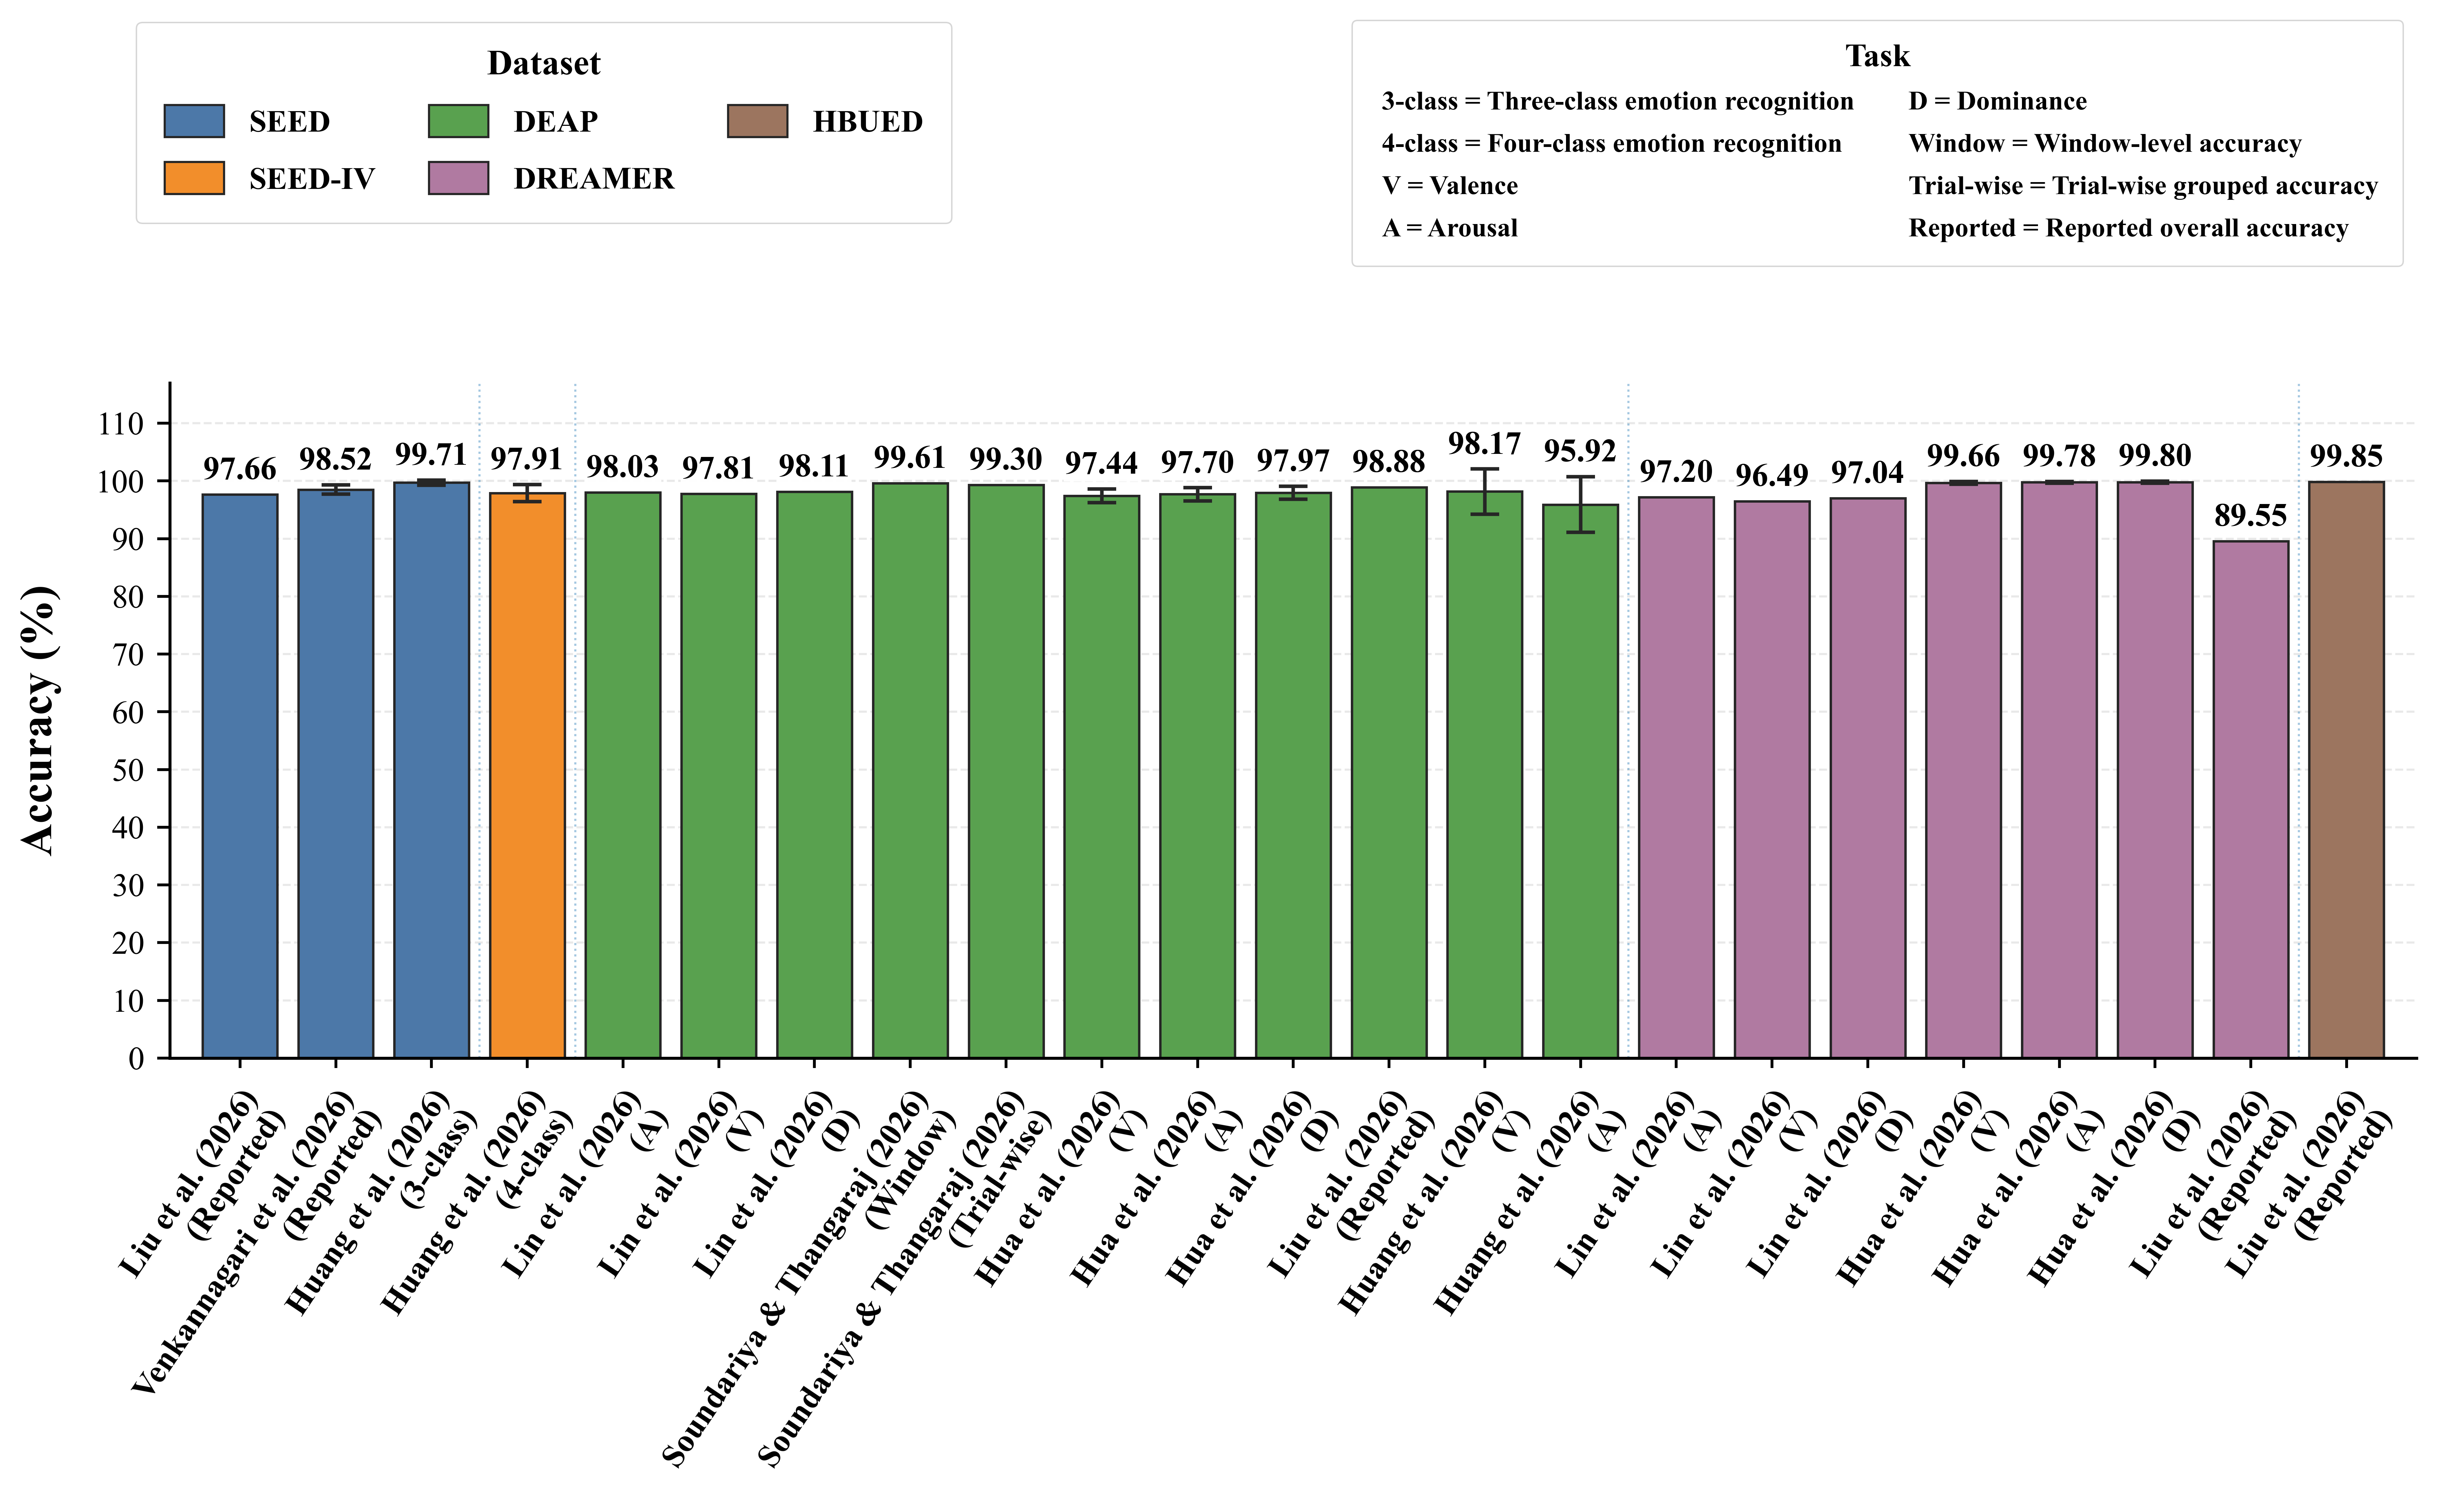
\includegraphics[
    width=\textwidth,
    keepaspectratio
]{pictures/subject_dependent.png}
\caption{Subject-dependent EEG emotion recognition accuracy across datasets, with error bars indicating reported standard deviations. Differences in experimental protocols limit direct comparability across datasets.}
\label{fig:subject_dependent_accuracy}
\end{figure*}


Subject dependent performance of EEG based emotion recognition has been visualized comparatively in Fig. ~\ref{fig:subject_dependent_accuracy} for six recent studies conducted on five standard datasets, i.e., SEED, SEED-IV, DEAP, DREAMER, and HBUED. The classification accuracy has been illustrated for various deep learning models used in those experiments. The experiments include binary classification of affective dimensions, multi class classification of emotions, and either window level or trial level classification of the data. The result shows that recently proposed subject dependent methods often have very high classification accuracy, which proves the efficiency of learning specific EEG spatial, spectral, and temporal representations for subjects.

Of the methods that use structured spatial representations, Lin et al.~\cite{lin2026pconvcapsnet} proposed PconvCapsNet, achieving 98.03\%, 97.81\%, and 98.11\% accuracy for the recognition of arousal, valence, and dominance, respectively, on DEAP. The accuracies of DREAMER on the same datasets are 97.20\%, 96.49\%, and 97.04\%. In addition, Huang et al.~\cite{huang2026astclnet} proposed AST-CLNet, using adaptive spatio temporal graph convolution and contrastive learning, achieving 99.71$\pm$0.45\% and 97.91$\pm$1.49\% accuracy on SEED and SEED-IV, respectively. On DEAP, the method achieved $98.17\pm3.91$\% for valence and $95.92\pm4.81$\% for arousal classification. These findings illustrate the potential of architectures that explicitly model EEG channel relationships and temporal dependencies, although their relative effectiveness cannot be established from heterogeneous evaluation protocols alone.

Attention and hybrid methods have also shown good results depending on the subject. Hua et al. proposed BRAD-Net, a model that incorporates brain region constrained attention together with complementary spatio temporal and spectral spatial features. The accuracy achieved by this model was in the range of $97.44\pm1.19$\% - $97.97\pm1.14$\% per each of the three emotional axes on DEAP, and for valence, arousal, and dominance on DREAMER, it attained $99.66\pm0.22$\%, $99.78\pm0.14$\%, and $99.80\pm0.16$\%, correspondingly. Soundariya and Thangaraj~\cite{soundariya2026awtnet} used the attentive wavelet transformer architecture and reported 99.61\% window level and 99.30\% trial level grouped accuracy on DEAP. It is particularly significant in terms of these two evaluation settings since the splitting of EEG signals affects classification performance.

Another example can be found from Liu et al.~\cite{liu2026taformer} who used their TaFormer model and obtained accuracies of 97.66\%, 98.88\%, 89.55\%, and 99.85\% on SEED, DEAP, DREAMER, and HBUED respectively. Inconsistencies between results on these datasets indicate the fact that good results on one dataset do not always mean good results on another dataset under other experimental conditions. The work of Venkannagari et al.~\cite{venkannagari2026robusteeg} reports 98.52$\pm$0.79\% accuracy on SEED with a framework for EEG classification using augmentations.

In aggregate, the findings depicted in Fig. ~\ref{fig:subject_dependent_accuracy} show that modern deep learning models are able to extract discriminative information regarding emotions from the EEG measurements on a per subject basis. Nevertheless, the prevalence of high classification accuracies cannot be considered as an unambiguous confirmation of cross subject performance. Divergent approaches used by different researchers to the selection of data samples, labeling of emotions, feature extraction, windowing and verification prevent the direct comparison of findings. In addition, the lack of standard deviations for some of the findings complicates performance analysis. Thus, the execution of trial independent testing and subject independent experiments becomes necessary for the determination of generalizability of the achievements mentioned.


The results demonstrate that subject dependent recognition has reached a high performance level on established benchmarks, particularly when spatial organization and frequency information are modeled jointly. On SEED, SFE-Net reports 99.19\%, exceeding the selected DGCNN and DCoT configurations under their respective reported protocols. The 2026 PconvCapsNet results are also consistently close to 98\% across the three DEAP dimensions and remain above 96\% across DREAMER, while simultaneously reducing convolutional computation through selective channel processing. These values, however, represent calibrated or within subject recognition and therefore should not be interpreted as evidence that equivalent performance will be preserved for previously unseen individuals.

\FloatBarrier

\subsubsection{Subject Independent Evaluation}
\label{subsubsec:subject_independent_evaluation}

Subject independent evaluation excludes the target participant from model training, commonly through leave one subject out or related subject wise partitioning. It therefore measures whether learned EEG representations capture emotion relevant characteristics that persist across individuals rather than relying on participant specific electrophysiological patterns. The substantial performance reduction observed for several architectures when moving from subject dependent to subject independent testing illustrates the importance of explicit generalization mechanisms.


\begin{sidewaystable*}[p]
\centering
\caption{Comparative overview of representative subject-independent EEG-based emotion recognition studies. A = arousal, V = valence, and D = dominance.}
\label{tab:subject_independent_results}
\scriptsize
\setlength{\tabcolsep}{2.5pt}
\renewcommand{\arraystretch}{1.12}
\begin{tabularx}{\textheight}{
>{\raggedright\arraybackslash}p{3.15cm}
>{\raggedright\arraybackslash}X
>{\raggedright\arraybackslash}X
>{\raggedright\arraybackslash}p{3.45cm}
>{\raggedright\arraybackslash}p{5.0cm}}
\toprule
\textbf{Study} &
\textbf{Input feature(s)} &
\textbf{Method} &
\textbf{Dataset / evaluation} &
\textbf{Accuracy (\%)} \\
\midrule
Song et al. \cite{song2020dgcnn} &
DE, PSD, DASM, RASM, and DCAU representations associated with EEG channels &
DGCNN with dynamically learned graph adjacency for modeling inter channel relationships &
SEED; subject independent &
79.95 \\
\lightrowsep
Li et al. \cite{li2023stgate} &
Electrode level spatial and time and frequency EEG representations &
STGATE combining spatial and temporal graph attention with a Transformer encoder &
SEED, SEED-IV, and DREAMER; subject independent &
SEED: $90.37 \pm 6.18$;
SEED-IV: $76.43 \pm 5.01$;
DREAMER-V: $77.44 \pm 8.40$;
DREAMER-A: $75.26 \pm 9.71$ \\
\lightrowsep
Dai et al. \cite{dai2025clra} &
Channel wise EEG temporal signals reorganized according to functional brain area relationships &
CLRA with 1D CNN and recurrent representation learning followed by brain area contrastive fusion &
DEAP and SEED; cross subject &
DEAP-V: 95.23;
DEAP-A: 96.31;
SEED: 95.16 \\
\lightrowsep
Chang et al. \cite{chang2025mshcl} &
Event related EEG representations organized at emotion and stimulus scales &
MSHCL using emotion scale and stimulus scale contrastive objectives in hierarchical hyperbolic space &
SEED, MPED, and FACED; cross subject &
SEED (3 class): 89.30;
MPED (7 class): 38.80;
FACED: 77.00 (binary), 45.70 (9 class) \\
\lightrowsep
Song et al. \cite{song2020iag} &
DE features from five frequency bands represented through channel and frequency graph structures &
IAG with sample dependent graph construction, multi level graph convolution,
graph coarsening, and recurrent modeling &
SEED; subject independent &
$86.30 \pm 6.91$ \\
\lightrowsep
Liu et al. \cite{liu2021decnn} &
Dynamic differential entropy obtained using empirical mode decomposition
and differential entropy &
DECNN integrating dynamic empirical decomposition with convolutional representation learning &
SEED; subject independent &
97.56 \\
\lightrowsep
Yin et al. \cite{yin2021gcnlstm} &
DE feature cubes generated after baseline calibration and temporal segmentation &
GCNNs extract graph domain features while LSTM captures temporal changes
in inter channel relationships &
DEAP; subject independent &
V: 84.81;
A: 85.27 \\
\lightrowsep
Li et al. \cite{li2021sognn} &
Time and frequency EEG channel features used to construct sample dependent electrode graphs &
SOGNN with dynamically self organized graph construction and graph convolution
for cross subject learning &
SEED and SEED-IV; cross subject &
SEED: $86.81 \pm 5.79$;
SEED-IV: $75.27 \pm 8.19$ \\
\lightrowsep
Priyasad et al. \cite{priyasad2022channelwise} &
Multichannel EEG processed with independent channel wise representation encoders &
Channel wise encoders coupled with geometric graph learning, multi head attention,
and multi channel feature fusion &
DEAP and DREAMER; cross subject &
DEAP: V 69.43, A 69.72, D 70.72;
DREAMER: V 64.98, A 63.71, D 61.81 \\
\lightrowsep
Gupta et al. \cite{gupta2019fawt} &
Channel specific EEG subbands obtained using flexible analytic wavelet transform,
followed by information potential features &
FAWT based subband decomposition, information potential feature extraction,
feature smoothing, and random forest/SVM classification &
SEED and DEAP; cross subject &
SEED (3 class): 90.48;
DEAP-V: 79.99;
DEAP-A: 79.95;
DEAP VA four class: 71.43 \\
\lightrowsep
Huang et al. \cite{huang2021bidcnn} &
Three EEG feature matrices constructed to represent baseline adjusted activity
and asymmetric responses of the left and right cerebral hemispheres &
BiDCNN with a three input CNN architecture for learning inter channel
and inter hemispheric differences &
DEAP; subject independent, disjoint training and testing subjects &
V: 68.14;
A: 63.94 \\
\lightrowsep
Fdez et al. \cite{fdez2021stratified} &
Multitaper spectral EEG features with participant based normalization
designed to suppress inter subject variability &
Feed forward neural network with stratified normalization applied
instead of conventional batch normalization &
SEED; cross subject evaluation &
91.60 (binary positive/negative);
79.60 (3 class positive/neutral/negative) \\
\lightrowsep
Wang et al. \cite{wang2022hslt} &
PSD features extracted from theta, slow alpha, alpha, beta, and gamma
frequency bands and organized according to EEG brain regions &
HSLT using electrode level and brain region level Transformer modules
to learn hierarchical spatial dependencies &
DEAP and MAHNOB-HCI; leave one subject out &
DEAP-A: $65.75 \pm 8.51$;
DEAP-V: $66.51 \pm 8.53$;
MAHNOB-HCI-A: $66.20 \pm 10.48$;
MAHNOB-HCI-V: $66.63 \pm 6.51$ \\
\midrule
\multicolumn{5}{r}{\textit{Continued on next page}} \\
\bottomrule
\end{tabularx}
\end{sidewaystable*}

\begin{sidewaystable*}[p]
\addtocounter{table}{-1}
\centering
\caption{Representative subject independent EEG emotion recognition results.}
\scriptsize
\setlength{\tabcolsep}{2.5pt}
\renewcommand{\arraystretch}{1.12}
\begin{tabularx}{\textheight}{
>{\raggedright\arraybackslash}p{3.15cm}
>{\raggedright\arraybackslash}X
>{\raggedright\arraybackslash}X
>{\raggedright\arraybackslash}p{3.45cm}
>{\raggedright\arraybackslash}p{5.0cm}}
\toprule
\textbf{Study} &
\textbf{Input feature(s)} &
\textbf{Method} &
\textbf{Dataset / evaluation} &
\textbf{Accuracy (\%)} \\
\midrule
Li et al. \cite{li2023gmss} &
DE features for SEED/SEED-IV and STFT based representations for MPED &
GMSS combining graph representation learning with spatial jigsaw,
frequency jigsaw, and contrastive self supervised auxiliary tasks &
SEED, SEED-IV, and MPED; subject independent &
SEED: $86.52 \pm 6.22$;
SEED-IV: $73.48 \pm 7.41$;
MPED: $28.49 \pm 4.42$ \\
\lightrowsep
Zhang et al. \cite{zhang2023sparsedgcnn} &
Multichannel frequency domain EEG features represented through
sparsified learnable electrode graphs &
SparseDGCNN using $L_1$ regularized graph connectivity and
forward and backward splitting to suppress redundant connections &
SEED, DEAP, DREAMER, and CMEED; subject independent &
SEED: 90.65;
DEAP-V: 64.66, DEAP-A: 66.65;
DREAMER-V: 68.18, DREAMER-A: 67.12;
CMEED-V: 66.83, CMEED-A: 75.47 \\
\lightrowsep
Ji et al. \cite{ji2026nrba} &
MIMO denoised multichannel EEG represented across principal frequency bands &
NR-BA-BFE-Net combining noise estimation, subspace filtering,
graph based band feature extraction, and band wise self attention &
SEED and SEED-IV; subject independent &
SEED: $95.56 \pm 4.18$;
SEED-IV: $83.15 \pm 3.40$ \\
\lightrowsep
Pandey and Seeja \cite{pandey2022vmd} &
Intrinsic mode functions obtained from EEG using variational mode decomposition &
VMD based feature decomposition followed by a deep neural network
for subject independent emotion classification &
DEAP; subject independent &
V: 62.50;
A: 61.25 \\
\lightrowsep
Jana et al. \cite{jana2022capsnet} &
Sparse spatio temporal EEG frames preserving electrode topology
and temporal variations of multichannel signals &
CapsNet trained on spatio temporal frame groups with leave one subject out
and unseen subject evaluation &
DEAP; cross subject &
LOO subject mean: 57.17;
unseen subject/unseen record mean: 51.07 \\
\lightrowsep
Xu et al. \cite{xu2023gruconv} &
Multichannel EEG sequences with temporal information retained from GRU units
before subsequent spatial representation learning &
GRU Conv combining GRU based temporal encoding with
CNN based spatial feature extraction &
SEED and DEAP; subject independent &
SEED: 87.04;
DEAP-A: 70.07;
DEAP-V: 67.36 \\
\lightrowsep
Yang et al. \cite{yang2019stsbssvm} &
Ten linear and nonlinear EEG feature families including spectral,
statistical, entropy, and Hjorth related descriptors &
ST-SBSSVM integrating significance testing, sequential backward
feature selection, and SVM classification &
DEAP and SEED; cross subject &
DEAP-V: 72.00;
SEED: 89.00 \\
\lightrowsep
Yin et al. \cite{yin2020lrfs} &
Candidate EEG features represented through subject specific probability
density functions to assess inter individual consistency &
LRFS using kernel density estimation, recursive feature elimination,
and ensemble classification across locally robust feature subsets &
DEAP and MAHNOB-HCI; individual independent &
DEAP-A: 65.10;
DEAP-V: 67.97;
MAHNOB-HCI-A: 67.43;
MAHNOB-HCI-V: 70.90 \\
\lightrowsep
Li et al. \cite{li2022mopso} &
Thirteen linear and nonlinear EEG features extracted using overlapping
4 s windows, followed by $L_1$ regularized feature selection &
Ensemble of selected base classifiers with weights optimized by
multiple objective particle swarm optimization &
DEAP and SEED; leave one subject out &
DEAP-A: 65.70;
DEAP-V: 64.22;
SEED: 84.44 \\
\lightrowsep
Bai et al. \cite{bai2023sect} &
PSD and DE frequency domain feature matrices upsampled using cubic spline
interpolation to retain relationships across EEG channels &
SECT combining a global channel Transformer with a shifted channel
Transformer for localized brain region representation learning &
SEED and DEAP; subject independent public dataset evaluation &
SEED (3 class): 85.43;
DEAP-V: 66.83;
DEAP-A: 65.31 \\
\lightrowsep
Su et al. \cite{su2023gapdpl} &
EEG feature representations projected into discriminative low dimensional
spaces through paired synthesis and analysis dictionaries &
GA-PDPL combining projection dictionary pair learning with genetic
optimization of model parameters &
SEED, MPED, and GAMEEMO; leave one subject out &
SEED: 69.89;
MPED: 24.11;
GAMEEMO binary: 64.34;
GAMEEMO four class: 49.01 \\
\lightrowsep
Guo et al. \cite{guo2024fcfan} &
Differential entropy features together with functional connectivity
representations calculated using phase synchronization &
FC-FAN using separate residual feature extractors, temporal
feature grouped attention, functional connectivity grouped attention,
and feature fusion &
SEED; cross subject &
$92.12 \pm 3.32$ \\
\lightrowsep
Kumar et al. \cite{kumar2026qpc} &
Nine bispectral quadratic phase coupling descriptors extracted from
frontal EEG rhythms, followed by genetic algorithm feature selection &
Explainable Boosting Machine using compact nonlinear bispectral
features under nested LOSO evaluation &
DEAP; nested leave one subject out &
A: 70.39;
V: 69.98 \\
\bottomrule
\end{tabularx}
\end{sidewaystable*}


Table~\ref{tab:subject_independent_results} summarizes representative subject independent EEG emotion recognition studies spanning graph based learning, convolutional and recurrent architectures, Transformer based modeling, contrastive representation learning, and conventional feature selection methods. Unlike subject dependent evaluation, these protocols examine the ability of learned representations to recognize emotional states in participants excluded from model training. The reported results reveal considerable variation across architectures and datasets, indicating that recognition performance depends not only on feature representation and model complexity but also on the characteristics of the evaluation protocol.

Graph based approaches demonstrate the importance of modeling spatial dependencies among EEG channels. DGCNN achieved 79.95\% accuracy on SEED, whereas SOGNN reported $86.81\pm5.79$\% on SEED and $75.27\pm8.19$\% on SEED-IV. Incorporating spatial and temporal graph attention with Transformer based representation learning, STGATE achieved $90.37\pm6.18$\% and $76.43\pm5.01$\% on SEED and SEED-IV, respectively \cite{li2023stgate}. More recent approaches report higher recognition rates under their respective experimental settings. NR-BA-BFE-Net obtained $95.56\pm4.18$\% on SEED and $83.15\pm3.40$\% on SEED-IV by integrating noise reduction, graph based frequency band representation learning, and attention mechanisms. These findings suggest that jointly modeling spatial relationships, frequency dependent characteristics, and noise related variability is a promising direction for cross subject emotion recognition.

Beyond graph oriented architectures, the results highlight the potential of alternative representations and learning strategies. DECNN reported 97.56\% accuracy on SEED using dynamic differential entropy representations, while CLRA achieved 95.16\% on SEED and reported 95.23\% for valence and 96.31\% for arousal on DEAP through brain area oriented contrastive representation learning \cite{liu2021decnn}. However, results on DEAP vary substantially across studies. BiDCNN reported 68.14\% for valence and 63.94\% for arousal, whereas the hierarchical spatial learning Transformer achieved $66.51\pm8.53$\% and $65.75\pm8.51$\%, respectively \cite{huang2021bidcnn}. Differences in feature construction, normalization, classification targets, subject partitioning, and experimental settings limit the validity of direct comparisons between these results. Furthermore, evaluations involving more emotion categories remain challenging. MSHCL reported 38.80\% accuracy on the seven class MPED task and 45.70\% on the nine class FACED task, illustrating the difficulties associated with more fine grained emotion classification.

\begin{figure*}[!t]
\centering
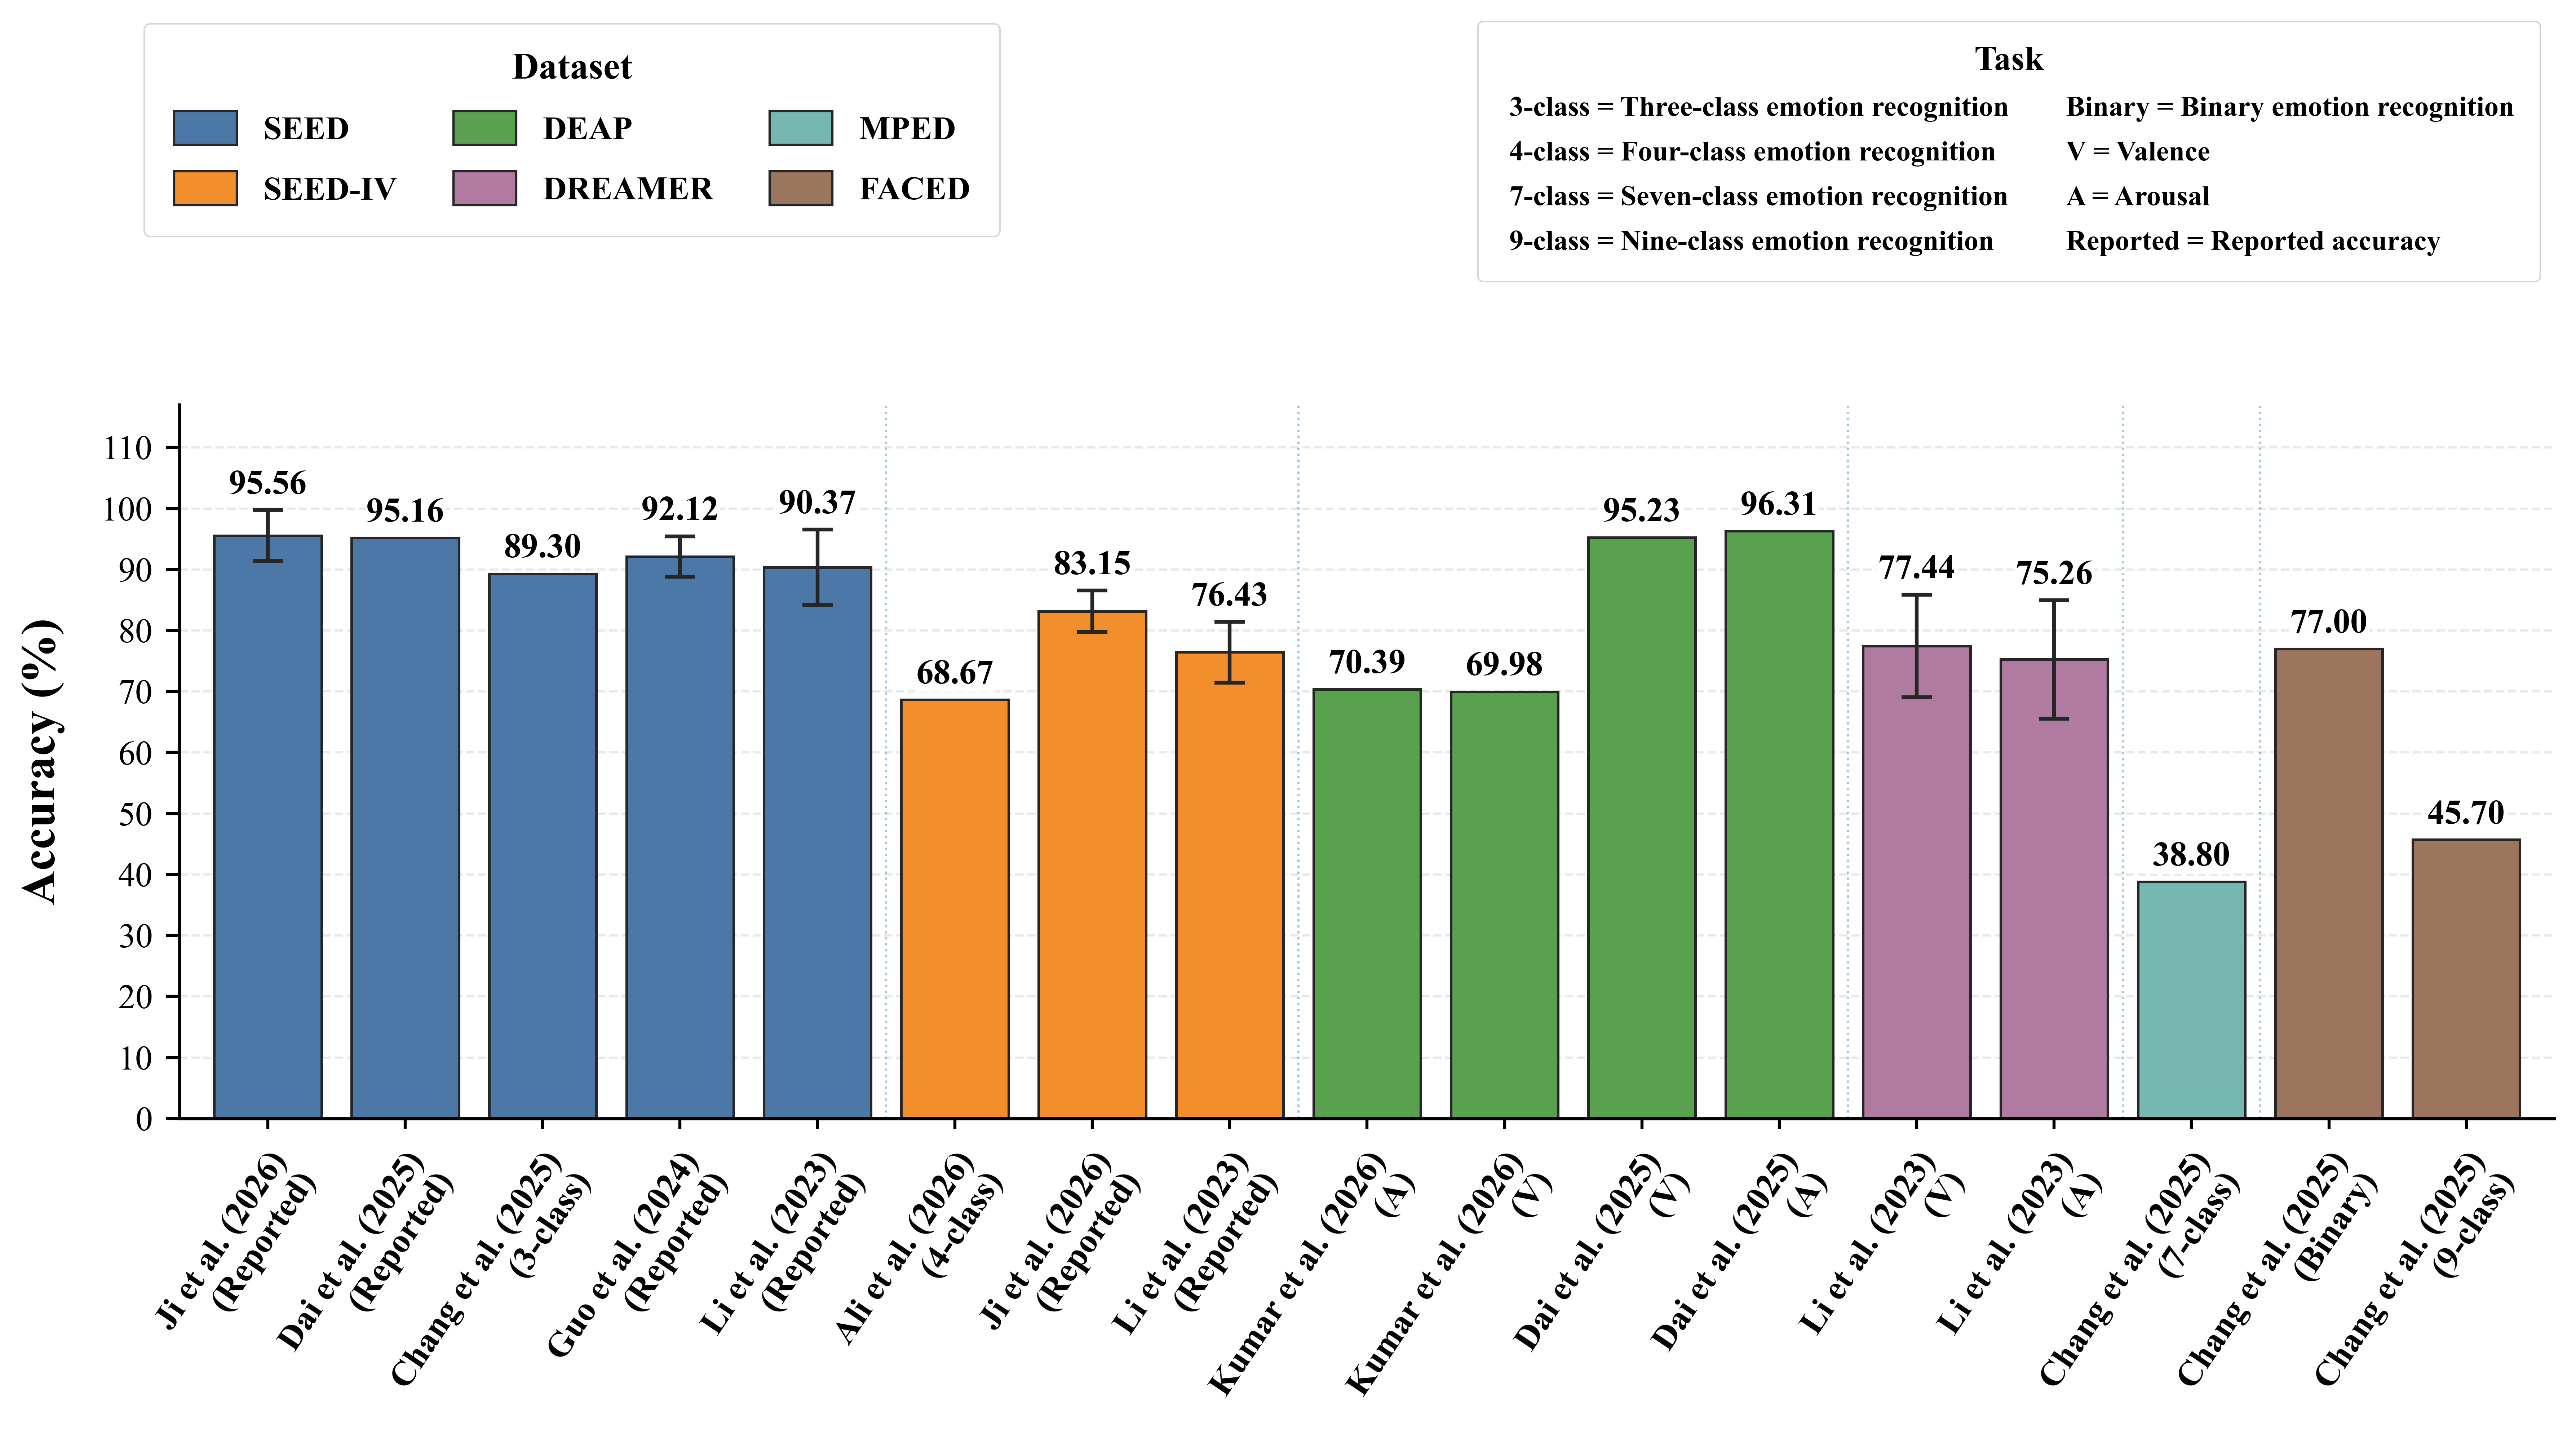
\includegraphics[
    width=\textwidth,
    keepaspectratio
]{pictures/subject_independent.png}
\caption{Subject-independent EEG emotion recognition accuracy across datasets, with error bars indicating reported standard deviations. Differences in experimental protocols limit direct comparability across datasets.}
\label{fig:subject_independent_accuracy}
\end{figure*}
\FloatBarrier
Overall, the results indicate that subject independent EEG emotion recognition benefits from representations capable of capturing informative spatial, spectral, and temporal patterns while reducing sensitivity to individual differences. Nevertheless, the considerable variability in reported accuracy, including among studies using the same datasets, prevents the identification of a universally superior architecture. Reliable comparisons therefore require consistent subject disjoint partitions, clearly documented preprocessing procedures, comparable emotion label definitions, and evaluation using complementary metrics such as macro F1 and balanced accuracy. These considerations also emphasize the importance of investigating transfer learning and domain adaptation as complementary strategies for improving recognition robustness across previously unseen EEG domains.





Fig. ~\ref{fig:subject_independent_accuracy} depicts the reported accuracy of seven latest EEG based emotion recognition studies on subject independent and cross subject evaluation scenarios. The comparison involves six benchmark datasets, namely SEED, SEED-IV, DEAP, DREAMER, MPED, and FACED, where the classification tasks include binary affective recognition and nine class emotion recognition. In contrast to the subject dependent evaluation scenario, where the training and test data could come from the same subject, subject independent evaluation evaluates the capability of the model in recognizing emotions from unseen subjects. The latter is very important due to the fact that distributional variations of neural activity, emotional reactions, and EEG signals could be different across individuals. As shown in the figure below, the reported accuracy varies greatly among different datasets, classification tasks, and models.

Recent models that combine graph based feature learning and attention mechanisms have shown impressive cross subject recognition results. As an example, Ji et al.~\cite{ji2026nrba} proposed NR-BA-BFE-Net, in which noise estimation, subspace filtering, graph based frequency band feature extraction, and band wise attention scheme are used. NR-BA-BFE-Net has an accuracy score of $95.56\pm4.18$\% on SEED and $83.15\pm3.40$\% on SEED-IV datasets. Another model is FC-FAN proposed by Guo et al.~\cite{guo2024fcfan}, which is differential entropy, functional connectivity, along with attention based feature fusion architecture.. FC-FAN achieves $92.12\pm3.32$\% accuracy on SEED dataset. Finally, Li et al. developed STGATE, which incorporates spatio temporal graph attention and Transformer based representation learning.This model has achieved accuracies of $90.37\pm6.18$\% on SEED and $76.43\pm5.01$\% on SEED-IV, in addition to $77.44\pm8.40$\% and $75.26\pm9.71$\% on valence and arousal recognition on DREAMER, respectively.

In addition, the approaches of contrastive representation learning and hybrid neural network architectures have been explored in order to enhance the classification of emotions independent of the subject. Dai et al.~\cite{dai2025clra} suggested the method of CLRA which combines the use of convolutional and recurrent feature extraction with contrastive fusion of brain area features and achieved 95.16\%, 95.23\%, and 96.31\% accuracies for SEED, DEAP valence, and DEAP arousal classification correspondingly. At the same time, the approach of MSHCL was developed by Chang et al.~\cite{chang2025mshcl} and uses the hierarchical contrastive loss functions in hyperbolic representation space and achieved 89.30\% for three class classification of SEED, 38.80\% for seven class classification of MPED, and 77.00\% and 45.70\% for binary and nine class classification of FACED, respectively. In particular, the distinction between binary and multi class tasks illustrates why classification accuracy should be interpreted with respect to the number of emotional categories and the corresponding evaluation protocol rather than considered independently of the experimental setting.

Other recent investigations have examined alternative feature representations and hybrid learning strategies. Ali et al.~\cite{ali2026hybridcnnlstmcbam} used the CNN and LSTM model with convolutional block attention mechanisms and attained 68.67\% accuracy on SEED-IV in a leave one subject out setting with 15 subjects and four emotions. Kumar et al.~\cite{kumar2026qpc} studied the use of compact nonlinear bispectral features with feature selection and Explainable Boosting Machine and achieved 70.39\% and 69.98\% accuracy on arousal and valence detection on DEAP dataset, respectively, using nested leave one subject out setting. The above studies show the wide range of approaches that have been applied to the problem of cross subject EEG emotion recognition. However, differences in validation procedures, feature extraction strategies, and target emotional dimensions prevent direct conclusions about the superiority of one architecture over another.

Overall, Fig. ~\ref{fig:subject_independent_accuracy} demonstrates that subject independent EEG emotion recognition remains a challenging and heterogeneous evaluation problem despite the encouraging results reported by several recent approaches. The variation witnessed through benchmarks highlights the fact that good classification results in one particular set do not guarantee generalized results in other sets or in other types of emotions. Additionally, variations in standard deviation data and the lack of uncertainty data in other cases make it difficult to assess model stability. In future research, it is recommended that there be emphasis on having subject disjoint evaluation, data regarding training and testing partitions, and performance measures for different classes in order to conduct statistical analyses using subjects withheld from experiments. These practices are important in proving the existence of generalization among subjects.

Subject independent results remain more variable because the classifier must operate under substantial person to person distribution shift. Transfer from multiple sources is highly effective in the chosen experiments, as seen in Quan et al. reporting 92.83\% on SEED while simultaneously evaluating DEAP and SEED IV \cite{quan2023bspc_multisource_transfer}. STGATE also demonstrates that jointly representing electrode topology and temporal dependencies can sustain useful performance across multiple datasets. Importantly, the 2026 CNN, LSTM and CBAM study reports a lower absolute value of 68.67\% on SEED-IV, but it employs a strict LOSO protocol across all 15 participants and four emotion classes, with PCA fitted exclusively on training subjects \cite{ali2026hybridcnnlstmcbam}. Thus, lower accuracy under a stricter unseen subject protocol should not be interpreted as inferior representation learning without accounting for the evaluation design.

\subsubsection{Transfer Learning}
\label{subsubsec:transfer_learning_evaluation}

Transfer learning explicitly addresses distribution mismatch by transferring useful emotion related knowledge from a source domain to a target domain. In EEG emotion recognition, the domain boundary may correspond to a recording session, an individual participant, or an entirely different dataset. These scenarios progressively introduce temporal, physiological, acquisition, and stimulus related discrepancies. Consequently, transfer learning methods have evolved from feature level distribution alignment toward multi source learning, calibration efficient adaptation, hybrid fine tuning, cross dataset unsupervised adaptation, and class conditional adversarial alignment.



\begin{sidewaystable*}[p]
\centering

\caption{Representative transfer learning evaluations for EEG based emotion recognition. Results correspond to the original transfer setting of each method; cross subject, cross session, and cross dataset results should therefore be interpreted separately. A = arousal and V = valence.}
\label{tab:transfer_learning_results}

\scriptsize
\setlength{\tabcolsep}{2.5pt}
\renewcommand{\arraystretch}{1.12}

\begin{tabularx}{\textheight}{
>{\raggedright\arraybackslash}p{2.65cm}
>{\raggedright\arraybackslash}p{3.15cm}
>{\raggedright\arraybackslash}X
>{\raggedright\arraybackslash}X
>{\raggedright\arraybackslash}p{3.8cm}
>{\raggedright\arraybackslash}p{5.25cm}
}

\toprule
\textbf{Category} &
\textbf{Study} &
\textbf{Input feature(s)} &
\textbf{Method} &
\textbf{Dataset / transfer setting} &
\textbf{Accuracy (\%)} \\
\midrule

Adversarial feature transfer &
Luo et al. \cite{luo2018iconip_wganda} &
Differential entropy EEG features &
WGAN based domain adaptation for learning transferable source and target representations &
DEAP and SEED; cross subject transfer &
DEAP-V: 67.99; DEAP-A: 66.85; SEED: 87.07 \\

\lightrowsep

Multi source domain adaptation &
Chen et al. \cite{chen2021frontiers_msmda} &
Five band differential entropy features from 62 EEG channels &
MS-MDA, treating individual source subjects as separate domains and aligning marginal distributions with the target &
SEED and SEED-IV; cross subject &
SEED: $89.63 \pm 6.79$; SEED-IV: $59.34 \pm 5.48$ \\

\lightrowsep

Hybrid DA and fine tuning &
Lu et al. \cite{lu2023frontiers_dffnet} &
Differential entropy features extracted from $\delta$, $\theta$, $\alpha$, $\beta$, and $\gamma$ bands &
DFF-Net combining an Emo-DA module with few shot target domain fine tuning &
SEED and SEED-IV; cross subject &
SEED: $93.37 \pm 1.88$; SEED-IV: $82.32 \pm 5.38$ \\

\lightrowsep

Conditional adversarial transfer &
Huang et al. \cite{huang2025ttcdan} &
DE and PSD features arranged as 14 s temporal sequences; each time step contains 310 features from 62 channels $\times$ five frequency bands &
TT-CDAN using a temporal Transformer, MMD based domain adapter, and conditional domain discriminator &
SEED and SEED-IV; cross subject &
SEED: 93.62; SEED-IV: 82.16 \\

\lightrowsep

Pseudo label propagation UDA &
Zhong et al. \cite{zhong2025daplp} &
Preprocessed emotion related EEG feature sequences from SEED, SEED-IV, and SEED-V, with temporal continuity exploited during propagation &
DAPLP combining global distribution alignment, reliable pseudo label selection, graph based label propagation, correction, and smoothing &
SEED, SEED-IV, and SEED-V; cross subject and cross session &
Cross subject: SEED 89.44, SEED-IV 74.57, SEED-V 69.15;
cross session: SEED 96.41, SEED-IV 82.20, SEED-V 84.70 \\

\lightrowsep

Cross dataset UDA &
Imtiaz and Khan \cite{imtiaz2025compbiomed_uda_gptds} &
Five band power spectral density features, DE was additionally evaluated in ablation experiments &
Unsupervised domain adaptation with gradual proximity guided target data selection and confidence aware test time augmentation &
SEED $\rightarrow$ DEAP and DEAP $\rightarrow$ SEED &
SEED$\rightarrow$DEAP: 59.68, DEAP$\rightarrow$SEED: 67.44 \\

\lightrowsep

Loop adversarial transfer &
Yan et al. \cite{yan2026latn} &
Electrode wise EEG feature matrices in which each sample contains $n$ electrodes and $d$ features per electrode &
LATN integrating structure aware associative alignment, inner/outer product combination, and semi supervised pseudo label selection to suppress negative transfer &
SEED, DEAP, and ECPL; cross subject &
SEED: 94.34;
DEAP-A: 89.21;
DEAP-V: 76.12;
ECPL: 96.33 \\

\lightrowsep

Riemannian geometric transfer &
Gao and Deng \cite{gao2026rgtgaa} &
SPD covariance matrices computed from local DE feature vectors and represented on a Log Euclidean manifold &
RGT-GAA combining a Log-Euclidean Graph Transformer with Fr\'echet mean geodesic alignment and adversarial domain adaptation &
SEED and DEAP; LOSO cross subject, cross session, and one to one transfer &
Cross subject: SEED 89.23;
DEAP-V: 66.40;
DEAP-A: 68.10;
cross session: 92.38;
one to one transfer: 74.56 \\

\lightrowsep

Multi source dendrite adaptation &
Liu et al. \cite{liu2026ddmsda} &
Five band DE features from $\delta$, $\theta$, $\alpha$, $\beta$, and $\gamma$ rhythms; 62 channel representations for SEED/SEED-IV and corresponding DEAP representations for cross dataset transfer &
DD-MSDA using a dendrite-net common feature extractor, domain specific branches, source to target and target to target MMD alignment, and multiple domain specific classifiers &
SEED, SEED-IV, and DEAP; cross subject, cross session, and cross dataset &
Cross subject: SEED 87.57, SEED-IV 74.79;
cross session: SEED 91.15, SEED-IV 75.57;
cross dataset average: 57.66 \\

\lightrowsep

Hierarchical adversarial transfer &
Hong et al. \cite{hong2026heat} &
Emotion evoked multichannel EEG representations from labeled source and unlabeled target subjects &
HEAT with hierarchical global/class conditional adversarial alignment and curriculum based progressive pseudo labeling &
SEED and SEED-IV; cross subject adaptation &
SEED: $95.37 \pm 5.17$; SEED-IV: $82.50 \pm 9.28$ \\

\midrule
\multicolumn{6}{r}{\textit{Continued on next page}} \\
\bottomrule

\end{tabularx}
\end{sidewaystable*}

\begin{sidewaystable*}[p]

\addtocounter{table}{-1}

\centering

\caption{Representative transfer learning evaluations for EEG-based emotion recognition.}

\scriptsize
\setlength{\tabcolsep}{2.5pt}
\renewcommand{\arraystretch}{1.12}

\begin{tabularx}{\textheight}{
>{\raggedright\arraybackslash}p{2.65cm}
>{\raggedright\arraybackslash}p{3.15cm}
>{\raggedright\arraybackslash}X
>{\raggedright\arraybackslash}X
>{\raggedright\arraybackslash}p{3.8cm}
>{\raggedright\arraybackslash}p{5.25cm}
}

\toprule
\textbf{Category} &
\textbf{Study} &
\textbf{Input feature(s)} &
\textbf{Method} &
\textbf{Dataset / transfer setting} &
\textbf{Accuracy (\%)} \\
\midrule

Multi source style transfer learning &
Li et al. \cite{li2020multisourcetl} &
Five band DE features extracted from 1 s EEG segments &
Multi source transfer with source selection, style transfer mapping between source and target EEG distributions, and source model integration, semi supervised variant exploits target test data transductively &
SEED; low resource cross subject transfer &
MS-S-STM: 88.92;
MS-Semi-STM: 91.31 \\

\lightrowsep

Wasserstein multi source adaptation &
Luo and Lu \cite{luo2021wmada} &
EEG feature representations extracted separately from multiple source subjects and the target subject &
wMADA $\beta$ with a shared feature extractor, source specific Wasserstein domain discriminators, and a common discriminator for multi source alignment &
SEED, unsupervised cross subject adaptation &
$89.30 \pm 4.00$ \\

\lightrowsep

Domain adaptive few shot learning &
Ning et al. \cite{ning2021dafsl} &
DE features from EEG channels spatially reorganized for convolutional representation learning &
Few shot transfer combining deep feature extraction, MMD source and target alignment, attention mechanisms, and prototype based target classification &
SEED and DEAP; five target samples per emotion category &
SEED: $96.51 \pm 1.49$;
DEAP: $64.55 \pm 6.65$ \\

\lightrowsep

Few label adversarial adaptation &
Wang et al. \cite{wang2021flada} &
EEG representations from selected source subjects plus a small labeled calibration subset from the target subject &
FLADA with source selection, six group adversarial source and target alignment, shared feature extraction, and classifier aggregation &
SEED and DEAP; low resource cross subject transfer &
SEED: $89.32 \pm 0.86$;
DEAP: $68.00 \pm 0.05$ \\

\lightrowsep

Prototypical pairwise transfer &
Zhou et al. \cite{zhou2023prpl} &
EEG feature representations from SEED and SEED-IV used to construct class prototypes and pairwise relationships &
PR-PL aligning source and target representations through prototypical learning and adaptive pseudo label based pairwise learning &
SEED and SEED-IV; cross subject and cross session cross subject transfer &
Session one cross subject: SEED $93.06 \pm 5.12$, SEED-IV $81.32 \pm 8.53$;
cross session cross subject: SEED $85.56 \pm 4.78$, SEED-IV $74.92 \pm 7.92$ \\

\lightrowsep

Pre trained cross dataset transfer &
Wang et al. \cite{wang2025pesd} &
EEG representations from emotionally sensitive source subjects across SEED, SEED-IV, DEAP, and FACED &
PESD pre trains a Vision Transformer encoder on emotion sensitive source data and transfers it using Mixup, triplet loss, and a domain discriminator &
SEED, SEED-IV, DEAP, and FACED; cross dataset transfer &
SEED: 93.14;
SEED-IV: 83.18;
DEAP: 93.53;
FACED: 92.55 \\

\lightrowsep

Two discriminator adversarial transfer &
Liu et al. \cite{liu2026tddann} &
310 D five band DE vectors ($62$ channels $\times$ $5$ bands) extracted from 0.5 s EEG segments &
TD-DANN with adaptive graph convolution, a source and target domain discriminator, and an individual discriminator for domain invariant and subject adaptive representations &
SEED and SEED-IV; cross subject domain adversarial transfer &
SEED: $89.45 \pm 5.87$;
SEED-IV: $77.13 \pm 7.97$ \\

\lightrowsep

Adaptive graph domain adaptation &
Luo et al. \cite{luo2026agcdan} &
DE features used to construct adaptive EEG graphs and dynamic frequency and spatial representations &
AGCDAN with multi branch source/target feature extraction, discriminator free marginal alignment, subdomain metric learning for conditional alignment, and decision fusion &
SEED, SEED-IV, and DEAP; multi source cross subject domain adaptation &
SEED: 89.68;
SEED-IV: 68.61;
DEAP: 68.13 \\

\lightrowsep

Flexible source aggregation &
Ran et al. \cite{ran2026fsanet} &
Multi source EEG representations dynamically aggregated according to source and target distribution similarity &
FSA-Net with similarity based source aggregation, global MMD alignment, local MMD plus contrastive subdomain adaptation, and domain aware weighted ensemble prediction &
SEED and SEED-IV; cross subject domain adaptation &
SEED: 90.80;
SEED-IV: 82.74 \\

\bottomrule

\end{tabularx}
\end{sidewaystable*}



Transfer learning in EEG based emotion recognition aims to improve the reuse of affective representations when the training and evaluation data differ across participants, recording sessions, or datasets. Rather than assuming identical feature distributions, these methods transfer information from source domains to a target domain through representation alignment, model adaptation, or limited target specific calibration. Table~\ref{tab:transfer_learning_results} summarizes representative approaches under their respective transfer settings.

The relevance of transfer learning arises from the considerable variability of EEG recordings across individuals and experimental conditions. Subject dependent models may exploit patterns specific to particular participants, whereas cross subject and cross session evaluation requires these patterns to remain informative in previously unseen data. Methods based on multi source learning, adversarial alignment, and feature distribution matching attempt to reduce such discrepancies, while calibration  and few shot based approaches additionally exploit limited target domain supervision. As shown in Table~\ref{tab:transfer_learning_results}, these strategies differ not only in model architecture but also in their assumptions about target domain data and labels.

The methods included in Table~\ref{tab:transfer_learning_results} illustrate the increasing diversity of transfer mechanisms. Adversarial and multi source approaches seek shared representations across subjects, while prototype based and pseudo labeling methods use class related structure to guide adaptation. More recent strategies incorporate Transformers, graph representations, curriculum based pseudo label refinement, and geometry aware alignment. Cross dataset experiments, including transfers between SEED and DEAP, examine a particularly challenging setting because differences in stimulus protocols, acquisition procedures, and participant populations may coincide. Such studies broaden evaluation beyond the more common within dataset cross subject scenario, although their reported accuracies remain dependent on the exact task and adaptation protocol.

Overall, the evidence in Table~\ref{tab:transfer_learning_results} suggests that transfer learning offers multiple practical routes toward more generalizable EEG emotion recognition. Nevertheless, accuracy values obtained under cross subject, cross session, cross day, few shot, and cross dataset conditions cannot be compared as a single ranking. Future evaluations should state the availability of target labels, adaptation stage access to target data, emotion class definitions, and partitioning rules to make the benefits and limitations of transfer strategies more transparent.

The transfer learning results show a clear methodological shift from global feature alignment toward class aware and target aware adaptation. Early WGAN based alignment already improved the feasibility of transferring DE representations across subjects, while multi source adaptation explicitly exploited differences among source participants rather than merging them into a single population. Calibration efficient PPDA reduced the amount of new user data required, whereas DFF-Net combined domain alignment with few shot fine tuning and reached 93.37\% on SEED and 82.32\% on SEED-IV.


The more difficult cross dataset setting remains substantially less accurate: the GPTDS/PC-TTA framework reported 59.68\% for SEED$\rightarrow$DEAP and 67.44\% for DEAP$\rightarrow$SEED despite explicitly addressing target reliability. This gap demonstrates that cross dataset transfer introduces additional mismatch from acquisition systems, subject populations, stimulus paradigms, and dataset construction. The 2026 HEAT framework reports 95.37\% on SEED and 82.50\% on SEED-IV by combining global and class conditional alignment with progressively selected pseudo labels \cite{hong2026heat}. Numerically, these reported within dataset cross subject results exceed the corresponding DFF-Net results on SEED and are slightly higher on SEED IV, although they should not be equated with cross dataset adaptation because the target domain discrepancy is fundamentally different. Overall, the experimental evidence indicates that increasingly fine grained alignment can substantially improve unseen subject recognition, whereas robust transfer across entirely different datasets remains the more demanding generalization problem.

\subsubsection{Brain Region, Channels and Frequency Band Importance}
\label{sssec:brain_region_channel_band_importance}
Emotion-related EEG activity is distributed across multiple cortical regions, electrodes, and frequency bands, reflecting interactions within broader neural networks rather than isolated activity. As illustrated in Fig.~\ref{fig:brain_regions}, frontal regions contribute to emotional evaluation and regulation, temporal regions support sensory and memory-related processing, and parietal and occipital regions participate in attentional and visual processing. Subcortical structures, including the amygdala, hippocampus, thalamus, and hypothalamus, further contribute to affective salience, contextual memory, neural communication, and autonomic regulation. However, emotional states emerge from coordinated interactions across these structures rather than anatomically isolated emotion-specific centers \cite{pessoa2017network}.


\begin{figure}[htb]
    \centering
    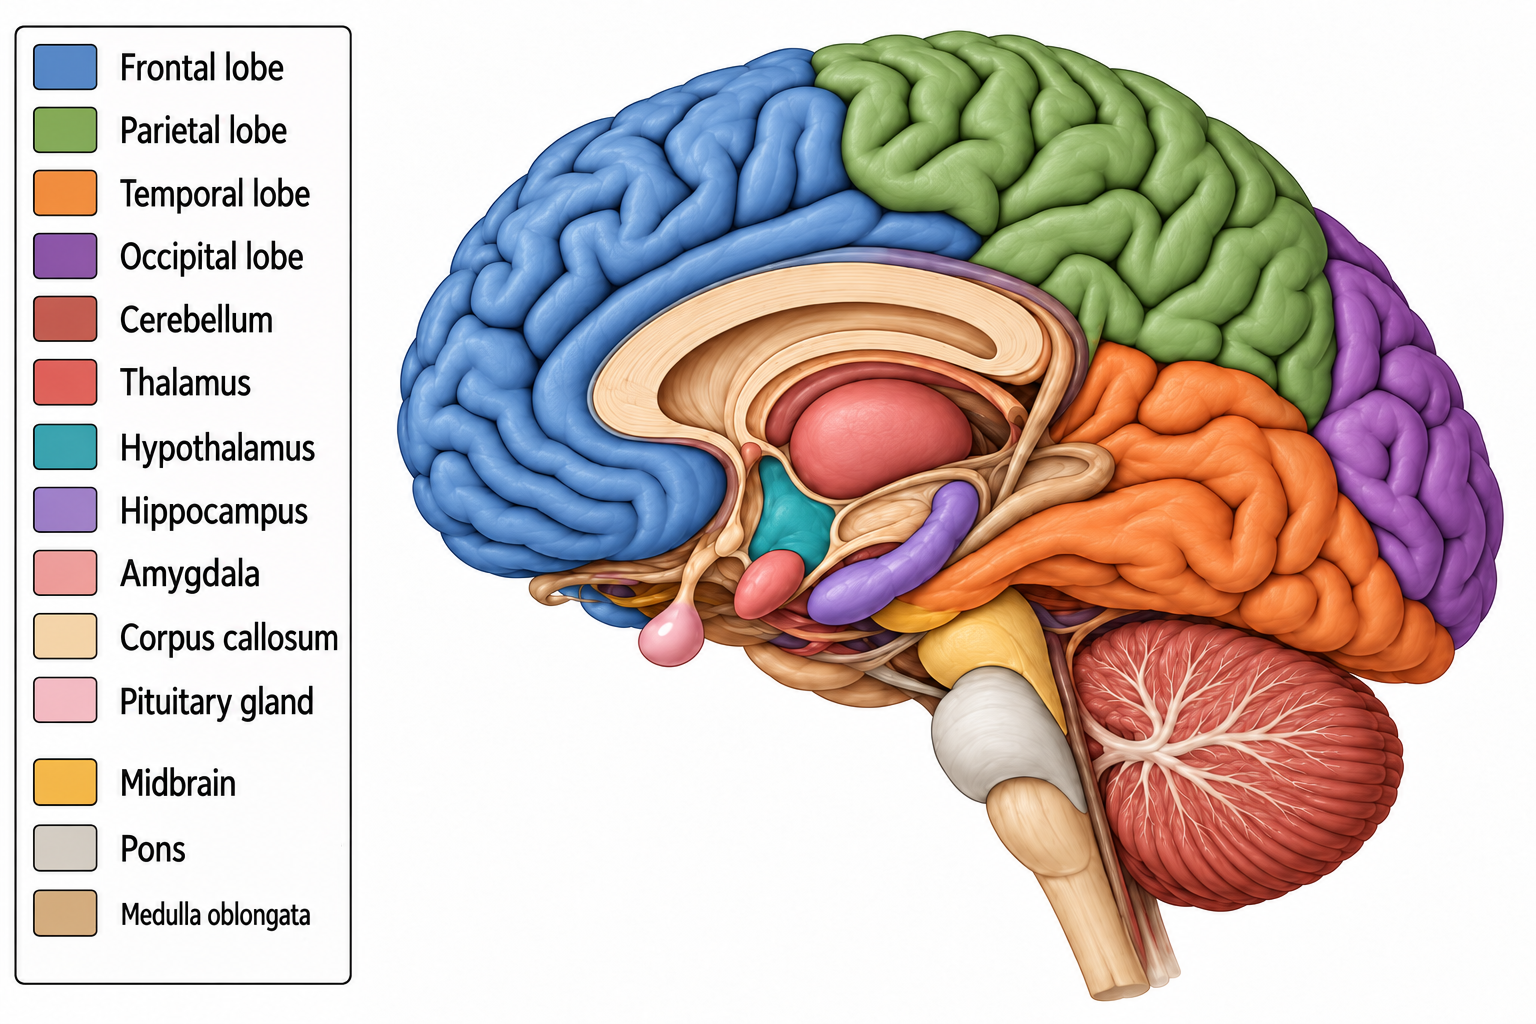
\includegraphics[width=\linewidth]{pictures/brain_regions.png}
    \caption{Anatomical overview of major brain regions associated with emotional processing, illustrating the frontal, parietal, temporal, and occipital lobes alongside subcortical structures, including the amygdala, hippocampus, thalamus, and hypothalamus, as well as the cerebellum and brainstem.}
    \label{fig:brain_regions}
\end{figure}


Understanding these distributed processes is essential for EEG-based emotion recognition because scalp EEG captures temporal, spectral, and spatial patterns associated with cortical neural activity. Nevertheless, its limited spatial specificity prevents reliable isolation of individual subcortical structures, requiring cautious anatomical interpretation \cite{cohen2017eegorigins}. Identifying informative electrodes, brain regions, and frequency components can improve computational efficiency and physiological interpretability. However, their relevance varies across subjects and recording conditions, making fixed channel or band selection potentially restrictive, particularly in subject-independent recognition \cite{brcfi_yang2024}.


\begin{small}
\begin{table*}[tp]
\centering
\setlength{\tabcolsep}{2pt}
\renewcommand{\arraystretch}{1.07}

\caption{Representative transfer-learning evaluations for EEG-based emotion recognition under the original experimental settings of each method. A = arousal and V = valence.}
\label{tab:brain_channel_band_importance}

\begin{tabularx}{\textwidth}{@{}
>{\raggedright\arraybackslash}p{0.1196\textwidth}
>{\raggedright\arraybackslash}p{0.1840\textwidth}
>{\raggedright\arraybackslash}p{0.1104\textwidth}
>{\raggedright\arraybackslash}X
>{\raggedright\arraybackslash}X
>{\raggedright\arraybackslash}X
@{}}

\toprule

\textbf{Study} &
\textbf{Method} &
\textbf{Dataset / Setting} &
\textbf{Brain Region and Channel Findings} &
\textbf{Frequency Findings} &
\textbf{Key Observation} \\

\midrule

Nakisa et al.~\cite{brcfi_nakisa2018} &
Evolutionary feature and channel selection &
DEAP, MAHNOB, mobile EEG &
Emotion related information was concentrated in selected rather than uniformly distributed electrodes. Prefrontal and parietal locations were prominent in DEAP, whereas central activity also contributed strongly in MAHNOB. Selected DEAP channels included Fp1, F7, FC5, AF4, CP6, PO4, O2, T7, and T8. &
$\alpha$ and $\gamma$ were prominent in DEAP, while $\alpha$, $\beta$, and $\gamma$ contributed substantially in MAHNOB. &
Spatial and spectral subsets differed across datasets, indicating that compact EEG configurations can preserve useful affective information without relying on the complete montage. \\

\lightrowsep

Kannadasan et al.~\cite{brcfi_kannadasan2023} &
Differential evolution based feature selection &
DEAP; subject independent &
Valence related features were concentrated mainly over frontal and parietal areas. Arousal additionally involved frontal and central electrodes. The selected channels differed between the two affective dimensions. &
$\alpha$ and $\beta$ contributed strongly to valence, whereas $\theta$, $\alpha$, and $\beta$ were informative for arousal. &
The study reported subject independent accuracies of 73.60\% for valence and 74.23\% for arousal, illustrating task dependent channel and band relevance. \\

\lightrowsep

Yang et al.~\cite{brcfi_yang2024} &
Learnable channel weighting and core graph extraction &
SEED &
Channel importance was learned directly rather than predetermined anatomically. The model identified a compact emotion relevant network by weighting EEG channels and pruning less useful nodes and graph connections. &
The work primarily addressed spatial channel importance rather than establishing a universal frequency band ranking. &
The method represents a transition from manually selected electrode subsets toward data driven discovery of task relevant EEG networks. \\

\lightrowsep

Valderrama \& Sheoran~\cite{brcfi_valderrama2025} &
Spatial and temporal attention &
SEED, SEED-IV, SEED-V; subject independent &
Repeatedly influential electrodes included Fp1/Fp2, F7/F8, T7/T8, P7/P8, and O1/O2. Their distribution indicates that emotion discriminative activity extends across frontal, temporal, parietal, and occipital regions. &
The analysis concentrated mainly on spatial channel relevance rather than identifying a single dominant spectral band. &
Mean subject independent accuracies were 79.3\%, 69.5\%, and 60.7\% for SEED, SEED-IV, and SEED-V, respectively. \\

\lightrowsep

Xu et al.~\cite{brcfi_xu2026uacl} &
Frequency aware self attention and uncertainty aware contrastive learning &
SEED, DEAP, DREAMER, FACED &
Multichannel EEG information was retained instead of selecting a fixed universal electrode subset. &
Frequency aware attention operates on real and imaginary frequency domain components. &
Reported accuracies reached 94.88\%, 98.71\%, 96.91\%, and 99.29\% on SEED, DEAP, DREAMER, and FACED, respectively. \\

\bottomrule

\end{tabularx}
\end{table*}
\end{small}


\begin{small}
\begin{table*}[tp]
\centering
\setlength{\tabcolsep}{2pt}
\renewcommand{\arraystretch}{1.07}

\addtocounter{table}{-1}

\caption{Representative findings on brain region, channel, connectivity, and frequency band importance in EEG based emotion recognition.}

\begin{tabularx}{\textwidth}{@{}
>{\raggedright\arraybackslash}p{0.1196\textwidth}
>{\raggedright\arraybackslash}p{0.1840\textwidth}
>{\raggedright\arraybackslash}p{0.1104\textwidth}
>{\raggedright\arraybackslash}X
>{\raggedright\arraybackslash}X
>{\raggedright\arraybackslash}X
@{}}

\toprule

\textbf{Study} &
\textbf{Method} &
\textbf{Dataset / Setting} &
\textbf{Brain Region and Channel Findings} &
\textbf{Frequency Findings} &
\textbf{Key Observation} \\

\midrule

Lin et al.~\cite{brcfi_lin2025brkds} &
Brain region knowledge and dual stream Transformer &
SEED, SEED-IV &
Electrodes were organized according to cortical regions instead of being treated as unrelated channels. Regional visualization indicated particularly useful information from temporal areas. &
Temporal, spectral, and spatial representations were jointly modeled rather than selecting one predefined EEG rhythm. &
The regional representation reduces dependence on exact electrode position and achieved 97.81\% on SEED and 90.76\% on SEED-IV. \\

\lightrowsep

Li et al.~\cite{li2021sognn} &
Self organized graph neural network &
SEED, SEED-IV; cross subject &
Learned graph structures emphasized frontal, temporal, central, and parietal locations. Nodes around FP2, F7, Cz, and CPz were among the informative areas, while inter electrode relationships were generated adaptively for different EEG samples. &
Among individually investigated rhythms, $\theta$ showed particularly useful discrimination, with $\beta$ and $\gamma$ also contributing. &
Adaptive graph construction achieved 86.81\% on SEED and 75.27\% on SEED-IV, supporting dynamic rather than fixed spatial connectivity. \\

\lightrowsep

Ma et al.~\cite{brcfi_ma2025sfswts} &
Spatial frequency shifted window attention &
SEED, SEED-IV &
Electrode topology was retained when EEG features were transformed into spatial frequency maps. Local and global relationships among electrode locations were learned through shifted window attention. &
Multiple frequency domain differential entropy components were jointly embedded instead of being evaluated as isolated bands. &
Joint spatial frequency modeling reported average accuracies of 99.46\% on SEED and 95.41\% on SEED-IV. \\

\lightrowsep

Hua et al.~\cite{hua2026bradnet} &
Brain region constrained attention &
DEAP, DREAMER; subject dependent and LOSO &
Electrodes were partitioned into anatomically meaningful regions. Attention was constrained mainly within corresponding brain regions, limiting physiologically implausible global interactions. &
A spectral spatial branch was combined with region constrained spatiotemporal modeling, allowing spectral and spatial information to complement each other. &
The architecture illustrates a recent trend toward combining learned attention with explicit neuroanatomical constraints for improved interpretability. \\

\bottomrule

\end{tabularx}
\end{table*}
\end{small}


As summarized in Table~\ref{tab:brain_channel_band_importance}, earlier studies emphasized frontal, temporal, and parietal activity alongside informative alpha, beta, and gamma rhythms. Recent approaches increasingly employ adaptive graph construction, channel attention, brain-region priors, and frequency-aware learning to capture complementary spatial--spectral relationships \cite{brcfi_lin2025brkds,brcfi_xu2026uacl}. Collectively, these findings support adaptive multiregional and multiband representations that preserve neurophysiological relevance while accommodating inter-subject variability and reducing redundant information.

\section{Discussion}
\label{sec:discussion}

The literature reviewed in this work shows that EEG based emotion recognition has progressed from conventional feature engineering pipelines toward increasingly sophisticated representation learning frameworks that model spatial, spectral, temporal, and inter channel dependencies. Nevertheless, improvements in reported classification accuracy do not translate directly into equivalent improvements in real world reliability. The central issue is that EEG emotion recognition is simultaneously a representation learning problem and a generalization problem: a model must identify affect related neural patterns while remaining robust to differences in participants, recording sessions, devices, experimental protocols, and environmental conditions. Recent systematic evidence likewise shows a persistent performance advantage for subject dependent evaluation over subject independent testing, indicating that individual variability remains a major obstacle to generalized affective decoding \cite{khare2024systematicemotionai,prabowo2023eegslr}.

This distinction is particularly important when interpreting the comparative results summarized in Tables~\ref{tab:subject_dependent_results} and \ref{tab:subject_independent_results}. Subject dependent models can exploit stable participant specific characteristics and therefore provide an important upper bound perspective on personalized recognition. Subject independent evaluation imposes a substantially more demanding requirement because the test participant is absent from model development, whereas transfer learning and domain adaptation approaches occupy an intermediate position in which information from source subjects is explicitly adapted to a new target domain. Consequently, reported accuracies should not be ranked without considering the associated subject partition, target data access, label configuration, session structure, and validation protocol. From this perspective, methodological progress should increasingly be judged not only by peak accuracy but also by robustness, calibration burden, computational feasibility, and the degree to which performance persists under realistic distribution shifts.

\subsection{Practical Implications and Real-World Applications}
\label{subsec:importance_practical_implications}

The practical importance of EEG emotion recognition arises from its capacity to introduce neurophysiological information into adaptive human computer and brain computer interaction. Unlike interfaces that rely exclusively on explicit commands, EEG informed systems can potentially infer changes in affective or cognitive state and use this information to modify system behavior. This capability is relevant to adaptive interfaces, assistive technologies, interactive environments, and multimodal affective systems in which EEG is combined with behavioral or physiological modalities. Reviews of EEG based BCI applications and multimodal emotion recognition systems consequently position affect sensitive neural interfaces as an important component of future context aware interaction, while also emphasizing that successful deployment depends on usability, portability, and robust operation outside tightly controlled laboratory settings \cite{varbu2022bciapplications}.

The same technological foundation has implications for safety and learning environments. EEG has been investigated for continuous fatigue estimation in driving, where wearable acquisition can support the detection of physiological changes associated with declining alertness, the E-Key framework, for example, demonstrates the feasibility of integrating wearable EEG with fatigue monitoring and subject identification within a unified system \cite{xu2023ekey}. In educational environments, EEG based attention feedback has also been explored as a means of providing real time neurofeedback during learning tasks \cite{sethi2018attentionfeedback}. These examples should not be interpreted as evidence that emotion classifiers can be transferred directly to fatigue or attention without retraining. Rather, they illustrate a broader practical implication: advances in portable EEG acquisition, low latency preprocessing, representation learning, and individualized calibration developed for affective computing can contribute to a wider family of neuroadaptive systems.

Healthcare and personalized digital environments represent another important direction, although the clinical implications require especially cautious interpretation. EEG contains information relevant to functional brain organization, and systematic evidence has identified altered EEG connectivity patterns in depression, supporting continued investigation of EEG as a complementary neurophysiological measure rather than as a stand alone diagnostic instrument \cite{miljevic2023depressionconnectivity}. At the same time, virtual reality interventions are increasingly studied in mental health contexts, creating opportunities for closed loop systems in which EEG derived affective information could eventually help select or adapt immersive stimuli \cite{lipira2023vrmentalhealth}. EEG derived information has also been explored in recommendation systems, including neuro recommendation approaches that use brain responses to support personalized product selection \cite{panda2024neurorecommendation}. Together with the expanding use of EEG in immersive virtual environments \cite{choi2023immersivevr}, these applications suggest that the long term value of emotion recognition may lie less in assigning an isolated emotion label and more in enabling adaptive systems that respond continuously to changes in the user's internal state.

The practical significance of the field therefore depends on a transition from benchmark oriented classification toward reliable affect aware interaction. Such a transition requires models that preserve performance across individuals and contexts, operate with acceptable computational latency, tolerate imperfect wearable recordings, and provide outputs whose uncertainty can be interpreted by downstream systems. High within dataset accuracy remains scientifically useful, but the more consequential question is whether an affective model can support a safe and meaningful decision when the user, recording environment, or acquisition hardware differs from the conditions under which the model was developed.

\subsection{Key Challenges and Future Research Directions}
\label{subsec:limitations_future}

Despite substantial methodological progress, several limitations continue to restrict the generalizability and translational value of EEG emotion recognition. These limitations are interconnected rather than independent. Restricted datasets encourage model overfitting, overfitting can inflate subject dependent results, inter subject variability reduces generalized performance, and poor generalization increases the amount of calibration required before deployment. Meanwhile, practical systems introduce additional sources of noise, latency, and user variability that are typically absent from benchmark experiments. A productive future research agenda should therefore address dataset design, personalized modeling, generalized modeling, and deployment requirements as components of a single validation pipeline rather than as separate research problems.

\subsubsection{Dataset Diversity, Annotation, and Standardization}
\label{subsubsec:dataset_challenges}

Dataset design remains one of the most fundamental constraints on progress. Existing EEG emotion recognition research is concentrated around a relatively small number of benchmark datasets, and systematic reviews show that DEAP and SEED account for a disproportionately large share of experimental studies \cite{prabowo2023eegslr}. Although this concentration facilitates methodological comparison, it can also encourage optimization toward the statistical properties of a few established benchmarks. Many datasets were acquired using controlled laboratory elicitation, modest participant populations, fixed stimulus sets, specific electrode montages, and a limited number of emotion categories. Such conditions are valuable for experimental control but do not fully represent the variability expected in naturalistic affective states, where emotion intensity, mixed emotions, contextual factors, and spontaneous transitions are substantially more difficult to standardize.

A related challenge is heterogeneity across databases. Differences in sampling rate, electrode density, reference configuration, preprocessing, stimulus duration, segmentation strategy, emotional annotation, and class definition complicate direct cross dataset comparison. Reviews of automated EEG emotion recognition repeatedly identify variability in datasets, preprocessing, feature extraction, and evaluation methodology as barriers to reproducibility and broader generalization \cite{vempati2023automatedeegreview}. Future datasets should therefore place greater emphasis on transparent metadata, standardized reporting of acquisition and preprocessing parameters, subject wise split definitions, repeated session recordings, and demographically broader cohorts. Multi site and longitudinal acquisition would be particularly useful for separating emotion related neural information from participant , session , and device specific variation.

Future dataset development should also reconsider how emotional ground truth is represented. Restricting affect to a small set of discrete labels or binary high/low dimensions simplifies classification but may conceal transitional, ambiguous, or mixed emotional states. More fine grained labels, confidence or intensity measures, repeated self assessment, and combinations of dimensional and categorical annotations could provide richer supervision. Naturalistic and immersive elicitation paradigms may further help bridge the gap between laboratory stimuli and real world affect, provided that the increased ecological validity is accompanied by careful control of movement, sensory load, and recording artifacts. The objective should therefore not be to maximize dataset size alone, but to increase the diversity of subjects, sessions, contexts, and emotional conditions in a way that meaningfully tests generalization.

\subsubsection{Subject-Specific Modeling and Personalization}
\label{subsubsec:subject_specific_challenges}

Subject dependent modeling remains valuable because it can exploit stable electrophysiological characteristics that are specific to an individual. As shown in Table~\ref{tab:subject_dependent_results}, many modern architectures obtain strong within subject performance by combining spatial topology, frequency domain information, temporal dependencies, graph representations, or attention mechanisms. Such results demonstrate that emotional information can be extracted effectively when the model is allowed to learn participant specific distributions. However, they primarily characterize personalized recognition and should not be interpreted as equivalent evidence of performance for previously unseen users.

A central methodological difficulty is that the quantity of data available for a single participant is usually limited relative to the capacity of contemporary deep networks. Increasing architectural complexity can therefore improve feature extraction while simultaneously increasing susceptibility to participant specific overfitting. Future subject specific systems should emphasize efficient personalization rather than unrestricted model complexity. Promising directions include compact hybrid architectures that integrate complementary spatial, spectral, and temporal representations, parameter efficient adaptation, representation pretraining followed by limited personalization, and explicit regularization of highly expressive attention or graph modules. More generally, systematic evidence suggests that multimodal and feature fusion strategies can provide complementary information, but the resulting models must be evaluated against their additional computational and data requirements rather than accuracy alone \cite{khare2024systematicemotionai}.

Personalized modeling should also incorporate temporal stability as an explicit evaluation criterion. A model trained and evaluated within one recording session may perform well while remaining sensitive to electrode placement, impedance, mood baseline, fatigue, or physiological changes on another day. Repeated session validation is therefore necessary to determine whether a ``subject specific'' model represents enduring affective characteristics or merely session specific signal structure. Future personalized systems would benefit from calibration procedures that update only the components required to accommodate session drift while retaining previously learned affective representations, thereby reducing the amount of new labeled EEG required for each use.

\subsubsection{Generalization Across Domains}
\label{subsubsec:generalized_modeling_challenges}

Generalized emotion recognition is more difficult because EEG distributions can vary substantially between individuals. Differences in anatomy, scalp conductivity, electrode contact, baseline oscillatory activity, cognitive appraisal, emotional regulation, and stimulus interpretation can all alter the observed signal without necessarily implying a different affective state. Consequently, a feature that is discriminative within one participant may be unstable when applied to another. Reviews of EEG emotion recognition systems consistently identify this inter individual variability as a principal reason why subject independent performance remains below subject dependent performance across many benchmark settings. This generalization gap is particularly important because practical systems cannot usually assume that a fully personalized model and a large labeled calibration dataset will be available for every new user.

Future work should therefore distinguish clearly between different forms of generalization. Pure subject independent evaluation should retain complete separation between training and test participants and should not be conflated with algorithms that access target subject data during adaptation. Unsupervised domain adaptation may use unlabeled target data, semi supervised adaptation may use limited labeled calibration, and domain generalization methods attempt to operate without target domain access. Cross session and cross dataset experiments introduce additional levels of distribution shift. Reporting these settings separately, as in Table~\ref{tab:subject_independent_results}, is essential because they answer different scientific questions.

The next stage of generalized modeling should move beyond optimizing a single benchmark split toward hierarchical stress testing. A model may first be evaluated using leave one subject out validation, then across sessions, acquisition devices, electrode subsets, and ultimately independent datasets. Transfer learning, domain adaptation, invariant representation learning, and source free adaptation can then be assessed according to how much target information they require and whether adaptation remains stable when source and target distributions differ substantially. Collaborative approaches such as federated or privacy preserving learning may also become valuable when multi institutional EEG data cannot be centralized. Importantly, generalized models should report not only overall accuracy but also class balanced measures, variability across held out participants, and failure cases, an improvement in mean performance has limited practical value if recognition becomes unreliable for a substantial subset of users.

\subsubsection{Real-World Deployment, Safety, and Ethical Considerations}
\label{subsubsec:practical_application_challenges}

Real world deployment introduces constraints that are largely absent from offline benchmark studies. Wearable EEG systems must contend with movement artifacts, changing electrode contact, environmental electrical noise, limited channel counts, setup time, user comfort, computational latency, and battery or hardware limitations. These factors interact directly with algorithm design: models that depend on dense electrode arrays, lengthy preprocessing, or repeated calibration may be unsuitable even if they achieve high laboratory accuracy. Reviews of EEG based BCI applications therefore emphasize portability and practical usability as central requirements for broader adoption \cite{varbu2022bciapplications}. Immersive environments introduce additional challenges because head and body movement, visually complex stimuli, and the interaction between EEG hardware and head mounted displays can alter recording conditions, the EEG VR literature consequently identifies experimental design and technical integration as continuing areas for improvement \cite{choi2023immersivevr}.

Deployment also raises questions that cannot be resolved by classification performance alone. An affect sensitive system may influence recommendations, educational feedback, safety alerts, or therapeutic content, meaning that erroneous predictions can alter the user's experience or subsequent behavior. Models should therefore communicate uncertainty, avoid presenting probabilistic affect estimates as definitive psychological judgments, and include mechanisms for user control and disengagement. These concerns become especially important in mental health applications. Although VR based psychological interventions have shown promise across several conditions, the evidence remains heterogeneous and further clinical validation is required before such systems can be treated as established therapeutic replacements \cite{lipira2023vrmentalhealth}. EEG emotion recognition should accordingly be positioned as a complementary sensing technology within professionally validated clinical workflows rather than as an autonomous diagnostic authority.

Privacy and ethical governance will become increasingly important as affective BCIs move toward continuous or personalized use. EEG contains information beyond the specific emotion label targeted by a classifier, and persistent neural data therefore require strong safeguards for consent, storage, transmission, secondary use, and model updating. Application oriented research should incorporate these considerations during system design rather than after model development. Real time validation should also evaluate how systems behave when signals are noisy, when confidence is low, and when users intentionally disengage. These requirements favor models that are not merely accurate, but also computationally efficient, interpretable at an appropriate level, uncertainty aware, and capable of failing safely.

Overall, the future of EEG based emotion recognition depends less on incremental improvements to benchmark accuracy than on closing the gap between controlled experimental performance and dependable use across people, sessions, devices, and environments. Larger and more representative datasets, carefully separated evaluation protocols, efficient personalized models, stronger cross subject generalization, and application aware validation should therefore be pursued jointly. Progress along these dimensions would shift the field from demonstrating that emotional information can be decoded from EEG toward establishing when, for whom, and under what conditions such decoding is sufficiently robust to support meaningful real world decisions.


\section{Conclusion}
\label{sec:conclusion}
The presented review offers an integrated analysis of emotion recognition based on EEG, uniting the psychological and neurophysiological background of emotions with the process of experimental design, EEG recording, signal processing, feature extraction, classification and evaluation. In contrast to method-focused reviews, this work discusses the impact of all these aspects and their interaction on the performance of emotion recognition, its reliability and generalization. Traditional approaches and deep learning techniques, data augmentation, transfer learning and domain adaptation are considered in terms of their importance for dealing with data scarcity and variability of different subjects. Special attention is paid to the difference between subject-dependent recognition performance and generalization to new subjects and datasets. Reproducibility of experiments and evaluation methods are discussed, as well. Such a perspective allows understanding the existing trade-offs in methodology and limitations of EEG-based emotion recognition. Future work should be concentrated on the development of evaluation protocols, cross subject and cross dataset generalization and computationally efficient methods.


\bibliography{references}
\end{document}
